\documentclass[12pt,PhD]{Thesis}
%%%% \documentclass[12pt,MSc,singlespace]{muthesis}
%%%%  can be used until the final draft
\usepackage{graphicx}
\usepackage{braket}
\usepackage{afterpage}
\usepackage{amssymb}
\usepackage{amsmath}
\usepackage{epstopdf}
%\usepackage{axodraw}
\usepackage{epsfig}
\usepackage{subfigure}
\usepackage[british]{babel}
\newcommand{\Pom}{I$\!$P}
\newcommand{\Reg}{I$\!$R}

\submitdate{2006}

% \renewcommand{\topfraction}{0.9}
 %\renewcommand{\bottomfraction}{0.8}
 %\setcounter{topnumber}{2}
  %  \setcounter{bottomnumber}{2}
 %   \setcounter{totalnumber}{4}     % 2 may work better
%    \setcounter{dbltopnumber}{2}    % for 2-column pages
%    \renewcommand{\dbltopfraction}{0.9} % fit big float above 2-col. text
%    \renewcommand{\textfraction}{0.07}  % allow minimal text w. figs
%    %   Parameters for FLOAT pages (not text pages):
%    \renewcommand{\floatpagefraction}{0.7}      % require fuller float pages
%        % N.B.: floatpagefraction MUST be less than topfraction !!
%    \renewcommand{\dblfloatpagefraction}{0.7}   % require fuller float pages
  %  \linespread{1.6}
\dept{School of Physics and Astronomy}
\begin{document}
\title{Central Exclusive Production at TeV Energies}
    \author{Andrew Denis Pilkington}
    \principaladviser{Prof. Fred Loebinger and Dr. Brian Cox}
%    \firstreader{John Green}
%    \secondreader{John BigBooty\\(Another School)}


%\renewcommand{\baselinestretch}{1.6}
%\parskip 8 true pt
%\parindent 25pt
\beforeabstract
\prefacesection{Abstract}
    Wakefields and the corresponding frequency-domain phenomenon beam coupling impedance have been well studied for a number of years as a source of beam instabilities within particle accelerators. With the development of the Large Hadron Collider (LHC) and the large beam currents stored in the LHC during fills for physics production, wakefield driven instabilities and strong beam induced heating have become a limiting factors in luminousity production due to both instantaneous luminousity and the available time for collisions.

In this thesis is presented an in depth study of the beam coupling impedance of two important (from both an impedance and operational point of view) pieces of equipment in the LHC; the collimation system and the injection kicker magnets (MKIs). These systems have both been sources of concern for the beam impedance of the LHC, the collimators due to their large transverse impedance and the MKIs due to the strong heating observed during the systematic increase of beam current during operation in 2011 and 2012. The source of the heating for the MKIs is studied in depth, found to be power lost by the beam to wakefields in the MKIs. Simulations and measurements are used to characterise the impedance and localise the components responsible for the high impedance, here the beam screen of the magnet, for which improvements are proposed and verified. A new RF damping system using ferrite for the collimation system is studied and compared to the existing RF damping system, focusing on the heating of the damping system. Highlights include a new method for measuring the quadrupolar and constant transverse impedances of an asymmetric structure using a coaxial wire technique is proposed and verified using computational simulations, and a study of the heat loss in a ferrite damped cavity, focusing on the location of the power loss for cavities being damped to varying degrees. 
\afterabstract
    \prefacesection{The Author}
    The author was educated at Winstanley College, Wigan, between 1997 and 1999, before obtaining a first class MPhys (Hons) degree at the University of Manchester. The work presented in this thesis was undertaken at the University of Manchester.

    \prefacesection{Acknowledgements}
     %acknowledgements here
    I would like to start by thanking my supervisors, Fred Loebinger and Brian Cox, for the encouragement and support they have given me over the past three years. This has been a great project to be part of and I am grateful that they let me work on it in a way that suited me best. I would also like to thank Jeff Forshaw for patiently explaining the theory and for the words ``Well, why don't you just write your own Monte Carlo?". Thanks to James Monk, who then helped me do just that. Thanks also to PPARC for funding the studentship.

Everyone in the HEP group deserves a mention for making it an enjoyable place to work, but with space a factor I will limit myself (mainly) to those who occupied the ATLAS office - Sarah, Irina, Andres, Paul, James and Simon. I have not forgotten Chris and Will, they just deserve a special mention for always being available for skiing or the Belgian bar. Or both. Thanks to everyone who proof read any part of this thesis (far too many to mention). Thanks also, for various reasons, to Rob and Tim.

Away from the physics department, I would like to thank all those people who I have had the privilege to know during the last few years. Thanks to Conor, Rory, Mike, Fraser, Casey, Tom, McGreevy, Darragh, Avik, Adam and Chris for all the laughs. Thanks to my family (Di, Viv, Don) for their support. Special thanks to my Mum and Dad who have always believed the best of me, often despite evidence to the contrary! 

Finally, I would like to say a huge thank you to Aneela for all that she does for me. She is the person who  brightens up my day if anything goes wrong, be it large or small. She has supported me in every way for seven years and especially during the last few months when I have been writing this document. For this and more, I will always be grateful.
\afterpreface

    %\chapter{Introduction}

%\parskip 8 true pt
%\parindent 25pt

\chapter{Introduction}
\section{CERN and the Large Hadron Collider}

CERN (Organisation europeene pour la recherche nucleaire) is a particle physics laboratory near Geneva, Switzerland crossing the Franco-Swiss border between the Swiss commune of Meyrin and French town of Saint-Genis Pouilly. It was founded in 1952 with the creation of the Coseil Europ\'{e}en pour la Recherche Nucl\'{e}aire, which became the Organisation in 1954. It houses an accelerator complex (shown in Fig.~\ref{fig:CERN-acc-complex})

\begin{figure}
\label{fig:CERN-acc-complex}
\caption{The CERN accelerator complex, showing both the proton and lead accelerator chains from LINACs 2 and 3 up to the LHC. Different experimental uses are highlighted in the diagram.}
\end{figure}

\begin{enumerate}
\item{Introduction to CERN}
\item{Introduction to the LHC}
\item{Luminousity - The Operational Figure of Merit}
\begin{itemize}
\item{Peak Luminousity - Equation and factors that control it}
\item{Integrated Luminousity - Up time and availability is important}
\end{itemize}
\item{Beam Dynamics}
\begin{itemize}
\item{Optics and Transverse Beam Dynamics}
\item{Longitudinal Dynamics - Energy change in a cavity}
\item{Chromaticity and Dispersion}
\end{itemize}
\end{enumerate}


\chapter{Theoretical Motivation}
\section{The Standard Model of Particle Physics}
 
The Standard Model of particle physics is based on a principle of symmetry under space-time and gauge transforms. The space-time transforms are translations, rotations and Lorentz boosts. 
Lorentz symmetry implies that  
the scalar product 
\begin{equation}
x^{\mu} y_{\mu} = \eta_{\mu \nu} x^{\mu}y^{\nu}
\end{equation}
of two space-time vectors, $x$ and $y$, is unchanged by transformations of the type
\begin{equation}
x^{\mu} \rightarrow x^{\prime \mu} = \Lambda^{\mu}_{\nu} x^{\nu}
\end{equation}
where $\Lambda^{\mu}_{\nu}$ is a Lorentz transform and $\eta_{\mu \nu}$ is the Minkowski metric. 
%= (1,-1,-1,-1)$. 
Since these space-time transforms represent a change in co-ordinate system, it follows that the laws of physics must be invariant under space-time transforms.


The Standard Model lagrangian is intended to describe the fundamental consituents of matter and their interactions with each other. The currently observed particles are the
bosons that mediate the electromagnetic, weak and strong forces and the fermions. 
The fermionic matter content is split into the six quarks and six leptons. The quark sector is made up of the up, down, charm, strange, top and bottom quarks. The leptons are split into the charged leptons  (electron, muon and tau) and the three neutrinos. The neutrinos are the only fermions that do not have mass\footnote{When the Standard Model was first proposed, there was no evidence for neutrino mass and as such they were assumed to be massless. It should be noted however, that mass differences between the neutrinos have recently been observed \cite{Tagg:2006sx}.}
 while the photon and gluons, that mediate the electromagnetic and strong forces respectively, are also massless.
The electromagnetic force affects only electrically charged particles, the weak force is observed to violate parity and the leptons do not interact via the strong force. The resultant theory must reflect all of these properties.

The Standard Model is constructed by building a massless interacting theory and adding the particle masses at a later stage. The lagrangian density, $\mathcal{L}_{dirac}$, for massless spin 1/2 fields, $\Psi(x)$, is given by
\begin{equation}\label{diracL}
\mathcal{L}_{dirac} = \bar{\Psi}\left( i \gamma^{\mu}\partial_{\mu} \right) \Psi
\end{equation}
where $\gamma_{\mu}$ are the Dirac matrices which satisfy the anti-commutation algebra $\{\gamma^{\mu}, 
\gamma^{\nu} \} = 2g^{\mu \nu}$.
The gauge boson interactions with the fermions are added by requiring that the lagrangian be invariant under local transformations generated by the gauge group
\begin{equation}
 SU(3)_C \times SU(2)_L \times U(1)_Y .
 \end{equation}
The details of this requirement are outlined in the following sections, but further information is available in the literature \cite{Halzen:1984mc,Ellis:1991qj,Mandl:1985bg,Ross:1999gw}.


\subsection{$\bold{U(1)_Y}$ Gauge Symmetry}

Taking $U(1)_Y$ transforms as an instructive example, one notices that the lagrangian is invariant under global phase transforms of the type
\begin{equation} \label{u1}
\Psi(x) \rightarrow e^{-i\omega Y}\Psi(x)
\end{equation}
where the value of the hypercharge, Y, depends on the type of field.
However, when the phase transform is local ($\omega \rightarrow \omega(x)$) then the lagrangian is no longer invariant and has an additional piece
\begin{equation}
\Delta \mathcal{L} = Y \, \bar{\Psi} \gamma_{\mu} \left[\partial_{\mu} \, \omega(x) \right] \Psi .
%-iY \partial_{\mu} \omega(x) .
\end{equation}
This is not an ideal situation because the phase is not a physical observable. It seems inappropriate then, that the phase at a particular point in space-time should depend on 
the phase at  every other point in space-time. 
% It seems improbable that the lagrangian be symmetric only if the field is transformed at every point in space at the same time. 

%replace all this below with B's instead of A's? remove mass terms remove reference to QED?

It is possible to restore the symmetry of the lagrangian if the partial derivative, $\partial_{\mu}$, is replaced with the covariant derivative $D_{\mu}$,
\begin{equation}
\partial_{\mu} \rightarrow D_{\mu} = \partial_{\mu} + ig^{\prime}YB_{\mu}
\end{equation}
and require that the vector field, $B_{\mu}$, simultaneously transforms as
\begin{equation}\label{Maxwell}
B_{\mu} \rightarrow B_{\mu} + \frac{1}{g^{\prime}} \partial_{\mu} \omega(x) .
\end{equation}
under the gauge transformation.
Thus, to make the lagrangian invariant under gauge transforms, it is necessary to introduce a new field. As a consequence of all this, an interaction term has been introduced to the lagrangian,
\begin{equation}
\mathcal{L}_{int} = -g^{\prime}Y\gamma^{\mu} \bar{\Psi} B_{\mu} \Psi ,
\end{equation}
which implies that the spinor field, $\Psi$, interacts with the vector gauge field, $B_{\mu}$, with coupling strength, $g^{\prime}$.
%The vector field exists in its own right and therefore there must be a kinetic term in the lagrangian which can be used to ascertain the equations of motion. 
It is then important to look for other terms involving $B_{\mu}$ that can be incorporated into the theory. The only other possible renormalisable and gauge invariant term that can be included in the lagrangian is the kinetic term, 
%It is also worth noting that equation \ref{Maxwell} shows the same gauge structure as Maxwell's equations of classical electrodynamics. It is possible to then to include a kinetic term which tells us how the the vector field behaves with no interaction and arrive at the lagrangian of QED,
\begin{equation}\label{kineticterm}
- \frac{1}{4} F_{\mu \nu}  F^{\mu \nu} , %+ 
%\bar{\Psi}(x)\left( \gamma^{\mu} D_{\mu} - m \right) \Psi(x)
\end{equation}
where the field strength tensor, $F_{\mu \nu}$, is given by
\begin{equation}
F_{\mu \nu} = \frac{-i}{g^{\prime} Y} \, [D_{\mu},D_{\nu}] = \partial_{\mu} B_{\nu} - \partial_{\nu} B_{\mu} .
\end{equation}
Note that a mass term for the vector field, $\frac{m^2}{2} B_{\mu} B^{\mu}$, cannot be included as it is not invariant under the gauge transform given by equation \ref{Maxwell}. This holds for all the gauge fields of the Standard Model, implying that no gauge boson can have an explicit mass term in the lagrangian.
 
 \subsection{Non-Abelian Symmetry and $\bold{SU(3)_C}$}
 
 It is possible to include other interactions in the same way. The $U(1)_Y$ gauge transform is based on the field being transformed by a simple phase that is just a number at each point in space. However, there is no reason, if the field contains some internal degrees of freedom, that the phase cannot be more complicated. Fields that are invariant under SU(N) transforms have N internal degrees of freedom and transform as
 \begin{equation}
\Psi(x) \rightarrow \Psi^{\prime}(x) = e^{-i\omega^a(x) \bold{t}^a} \Psi(x)
\end{equation} 
 where the $\bold{t}^a$ are the $N^2 -  1$ generators of the group. These generators, $\bold{t}^a$, have a distinct algebra 
\begin{equation}
[\bold{t}^a,\bold{t}^b] = if^{abc}\bold{t}^c
\end{equation} 
which leads to some new features in the lagrangian when compared to the $U(1)_Y$ case. The functions $f^{abc}$ are the structure constants of the group. Each of the generators of SU(N) can be represented in terms of an $N\times N$ matrix (fundamental representation).  
 
In the case of $SU(3)_C$, the quarks are assigned an internal degree of freedom known as colour. This is motivated in part by the observation that, without colour,  some of the hadrons, such as $\Delta^{++}$, are symmetric under the interchange of the constituent quarks \cite{Halzen:1984mc}. This is forbidden by Fermi-Dirac statistics and a new degree of freedom is required to restore the anti-symmetric wave function. There are eight generators (represented by the Gell-Mann matrices) of the $SU(3)_C$ group and hence eight gauge fields are required to keep the lagrangian symmetric under gauge  transformations. The covariant derivative (now a $3\times3$ matrix which acts on a three component field) is given by
 \begin{equation}
 \bold{D}_{\mu} = \partial_{\mu}\bold{I} + ig_s \bold{t}^a G^a_{\mu}
 \end{equation}
 where $\bold{I}$ is the unit matrix, $g_s$ is the coupling strength and the gluon fields, $G^a_{\mu}(x)$, are the gauge fields 
 %which transform as
 %\begin{equation}
 %G^a(x) \rightarrow G^{\prime a}(x) = G^a(x) + \frac{1}{g}\partial_{\mu} \omega^a(x) - f^{abc} G^b(x) \omega^c(x).
 %\end{equation}
required to keep the lagrangian invariant under the SU(3) transform.
%\begin{equation}
%\Psi(x) \rightarrow \Psi^{\prime}(x) = e^{-i\omega^a(x) \bold{t}^a} \Psi(x).
%\end{equation} 
%what about the colour index??
%The extra piece in the transform of the gluon fields leads to some interesting results when the kinetic part of the lagrangian is evaluated. There are extra self-interaction terms 

As SU(3) is a non-abelian group, the field strength tensor, $F^a_{\mu \nu}$, has more structure than in the $U(1)_Y$ case and is  given by
\begin{equation}\label{su3fmunu}
F^a_{\mu \nu} = \partial_{\mu} G^a_{\nu} - \partial_{\nu} G^a_{\mu}
- g_s f^{abc} \, G^b_{\mu} G^c_{\nu}
\end{equation}
where the third term arises due to the algebra of the SU(3) group.
This in turn leads to extra terms when the kinetic part of the lagrangian (equation \ref{kineticterm}) is evaluated for the gluons. 
These are given by
 \begin{equation}
 \mathcal{L}_{int} = g_sf^{abc}(\partial_{\mu}G^a_{\nu})G^{b,\, \mu}G^{c, \, \nu} - \frac{1}{4}g_s^2f^{abc}f^{ade}G^b_{\mu}G^c_{\nu}G^{d, \, \mu}G^{e, \, \nu}
 \end{equation}
 which represent the self-interaction of three or four gluons respectively. This should be contrasted with the $U(1)_Y$ case, which contained no self interaction terms.
%something here to say wow, that is weird.
%next bit a bit hazy

The interaction terms in the lagrangian can be used to calculate the probability of a particular scattering process. For example, at leading order the coupling of two quarks and a gluon is described by the coupling strength, $g_s$, which appears in the lagrangian. In reality however, the measured coupling does not correspond to just the leading order term, but includes higher order (loop) corrections. This results in the running of the measured coupling, i.e $g_s \rightarrow g_s(\mu^2)$, where the momentum scale, $\mu$, defines the scale at which the coupling is measured. By convention, the measured parameter is the strong coupling, $\alpha_S$, 
which is defined as $4\pi \alpha_S = g_s^2$. %which is given by
%\begin{equation}
%\alpha_S = \frac{g_s^2}{4\pi}.
%\end{equation}
%Consider the perturbative calculation of quark-quark scattering via gluon exchange. Such a calculation involves the evaluation of loop corrections to the gluon propagator, as shown in figure \ref{gluonpropagator}. 
%The momenta of each line in the loop is not constrained and hence an integral over all possible momentum is required for the complete calculation. This, however, results in divergences in the calculation. The method for resolving this apparent problem is to recognise that the bare coupling, $g_s$, in the lagrangian is not the coupling that we observe experimentally. The divergences of the loop integral are absorbed into the strong coupling itself. This means that the coupling has been altered by the higher order corrections to the interaction, which in turn means that the coupling depends upon the momentum scale at which the interaction is evaluated. 
%In the case of the strong coupling, the renormalisation group equation is
%\begin{equation}
%\mu^2 \frac{\partial \alpha_S}{\partial \mu^2} = \beta ( \alpha_S ) 
%\end{equation}
%where $\mu$ is the momentum scale at which the ultraviolet subtractions of higher order terms are performed.
%The $\beta$ function is calculable in perturbative QCD and is given by
%\begin{equation}
%\beta(\alpha_S) = -b\alpha_S^2 \left( 1 + b^{\prime} \alpha_S + b^{\prime\prime}\alpha_S^2 + \mathcal{O}\left(\alpha_S^3\right) \right)
%\end{equation}
%where $b$, $b^{\prime}$ and $b^{\prime\prime\prime}$ are the constants applicable to one, two and three loop corrections respectively. Using one loop as an example, the renormalisation equation can be solved 
%between the scale of interest and a renormalisation scale, $\mu$ and results in
%\begin{equation} \label{alpha_mu}
%\alpha_S \left( Q^2 \right) = \frac{\alpha_S \left( \mu^2 \right)}{1 + \alpha_S \left( \mu^2 \right) b \ln { \left( %\frac{Q^2}{\mu^2} \right) }}
%\end{equation}
%which tells us how the coupling changes with scale but gives no prediction of the overall value. 
%It is possible evaluate the coupling 
%by introducing a parameter, $\Lambda$, which indicates where the coupling becomes infinite. 
%Solving the renormalisation equation now gives (for one loop)

In the one-loop approximation \cite{Ellis:1991qj}, the strong coupling is given by
\begin{equation} \label{alpha_la}
\alpha_S \left( \mu^2 \right) = \frac{12 \pi}{\left(33 - 2n_f \right)}\frac{1}{ \ln{\left( \frac{\mu^2}{\Lambda^2}\right)}}
\end{equation}
where the $n_f$ is the number of active quark flavours at that momentum scale. 
At the scale $\mu = \Lambda$, the coupling becomes infinite. This really means that the coupling is strong enough to make perturbation theory not applicable. 
%Non -perturbative quantities, such as hadron masses, should be at approximately the same scale, $\Lambda=160$MeV.
Infra-red slavery is the statement that, as $\mu \rightarrow \Lambda$, the interaction becomes so strong that the coloured objects are confined into colour neutral states. This qualitatively explains why coloured objects are not observed on large distance scales. Asymptotic freedom is the inverse statement that, at large $\mu$, the strong coupling becomes small and perturbation theory is applicable.

\subsection{$\bold{SU(2)_L}$ Symmetry}

The SU(2) transformations follow the SU(N) algebra. There are three generators, which can be represented (in the fundamental representation) by the Pauli matrices, and hence three gauge fields, $W^a_{\mu}(x)$, are required to keep the lagrangian invariant under the gauge transformation. The covariant derivative is now given by
%SU2 covariant derivative - need and explain W^+ W- made from W1,2
\begin{equation}
\bold{D_{\mu}} = \left(\partial_{\mu}\bold{I} + 
i\frac{g}{2} \left( 
\begin{array}{c c}
W^3_{\mu} & \sqrt{2}W^{-}_{\mu} \\
\sqrt{2} W^{+}_{\mu} & -W^{3}_{\mu}
\end{array}
\right) 
\right)
\end{equation}
with $g$ being the coupling strength. The $W^{\pm}$ are the bosons that mediate weak interactions such as muon decay and are given by
\begin{equation}
W^{\pm} = \frac{1}{\sqrt{2}} \left( W^{1}_{\mu} \pm iW^{2}_{\mu} \right).
\end{equation}
%The fermions are not assigned an new internal degree of freedom but are rather arranged into doublets which transform under SU(2). 

%The fermions are not assigned a new internal degree of freedom, but are arranged into doublets which transform under $SU(2)_L$. 
The fermions are rewritten as the sum of a left-handed and right-handed component, ($\Psi=\Psi_{R}+\Psi_{L}$), which can be obtained by the projection operators
\begin{equation}
P_{R,L} = \frac{1}{2}(1\pm \gamma^5),
\end{equation}
i.e $P_L \Psi = \Psi_L$.
The left-handed fermions are then assigned to doublets that transform under $SU(2)_L$. For example,
the left-handed components of the electron-neutrino and electron form a doublet, $L_e$, given by
\begin{equation}
L_e = \left(
\begin{array}{c}
\nu_{e, L} \\ e_L
\end{array}
\right) .
\end{equation}
The right-handed components however,  are not assigned into doublets and transform as scalars under $SU(2)_L$, e.g $e_R \rightarrow e_R$.
This is necessary because the final theory must reflect the observed `V-A' parity violations of the weak sector.

The different transformation properties of the left and right-handed fermions means that an explicit mass term for the fermion fields, $m \Psi \bar{\Psi}$, also cannot be included because this mass term will mix the right and left-handed components of the field. As such, the mass term would not be invariant under the $SU(2)_L$ gauge transform.
The hypercharge values also differ for the right and left-handed fermions and are given in table \ref{hypercharges}. The hypercharge assignments are carefully chosen so that, after the Higgs mechanism (described in the following section), the theory produces the correct couplings to the photon.

\begin{table}[t]
\centering
\begin{tabular}{|c|c|c|c|c|c|}
\hline
& & \multicolumn{3}{|c|}{Particle Type} & Hypercharge \\
\hline
& Quarks & $u$ & $c$ & $t$ & $1/6$ \\
Left &  & $d$ & $s$ & $b$ & $1/6$ \\
Handed & Leptons & $\nu_{e}$ & $\nu_{\mu}$ & $\nu_{\tau}$ & $-1/2$\\
& & $e$ & $\mu$ & $\tau$ & $-1/2$ \\
\hline \hline
& Quarks & $u$ & $c$  & $t$ & $2/3$\\
Right & & $d$ & $s$ & $b$ & $-1/3$\\
Handed & Leptons & & & &\\
& & $e$ & $\mu$ & $\tau$ & $-1$\\
\hline 
\end{tabular}
\caption[The hypercharge values of the Standard Model fermions]{The hypercharge values of the Standard Model fermions. The quarks are the up ($u$), down $(d)$, charm ($c$), strange, ($s$), top ($t$) and bottom ($b$). The leptons are the electron ($e$), muon ($\mu$), tau $(\tau$) and the associated neutrinos ($\nu$). \label{hypercharges}}
\end{table}%

\subsection{The Higgs Mechanism}

The prescription so far has been to incorporate gauge boson interactions into the lagrangian by requiring symmetry under gauge transforms. However, this means that none of the bosons or fermions can have an explicit mass term. % which goes against experimental evidence. 
%Furthermore, mass terms for the fermions are forbidden because of the chiral nature of the lagrangian; a $m\bar{\Psi}\Psi$ term would mix the left and right-handed components of the field and hence would not remain invariant under the $SU(2)_L$ transform. 
%higgs from here
In the Standard Model, the mass problem is solved by the introduction of a complex scalar field, $\Phi(x)$, which transforms as a doublet under $SU(2)_L$ and has hypercharge $Y(\Phi)=\frac{1}{2}$. The lagrangian for this field is 
\begin{equation}
\mathcal{L}_{scalar} = |\bold{D}_{\mu}\Phi|^2 - V(\Phi)
\end{equation}
where the covariant derivative is one appropriate to $SU(2)_L$ and $U(1)_Y$. The potential, $V(\Phi)$, is 
\begin{equation}\label{scalarpotential}
V(\Phi) = -\mu^2\Phi^{\dagger}\Phi +
\lambda\left(\Phi^{\dagger}\Phi\right)^2 
\end{equation}
and the minimum of this potential occurs at $\Phi^{\dagger}\Phi =  v^2 = \mu^2 / 2\lambda$ for $\mu^2 > 0$ and $\lambda > 0$. This means that the  new scalar field has a non-zero vacuum expectation value. The lagrangian is now no longer explicitly symmetric under transformations which simply move from one vacuum to a new one. The specific choice of a vacuum state is said to spontaneously break the gauge symmetry. 

%The field can be expanded about the expectation value, and is conventionally written as
%\begin{equation}
%\Phi = \left( 
%\begin{array}{c}
%\phi_1 + i\phi_2 \\
%v + H + i\phi_3 
%\end{array}\right).
%\end{equation}
%The fields $\phi_1$, $\phi_2$ and $\phi_3$ are said to be unphysical, which means that they are not observable. It is possible to gauge transform them away and write the field more simply as 
%Could just screw this bit off(above) and write in unitary gauge to start - mmm  i have done

The scalar field can be expanded about the expectation value and can be expressed, in the unitary gauge, as
\begin{equation} \label{cmplxdoublet}
\vspace{0.2cm}
\Phi =
\left( \begin{array}{c}
0 \\v + H
\end{array}
\right)
\vspace{0.2cm}
\end{equation}
where the Higgs field, $H$, is a physical field and cannot be removed by a different choice of gauge. If this form for the scalar field is used in the scalar potential term (equation \ref{scalarpotential}) there is, amongst other things, a mass term for the Higgs field with $m_H = 2\lambda v$. As $\lambda$ is  a free parameter, the Higgs mass is not predicted by the Standard Model.
 
When the scalar kinetic term is evaluated, there is a kinetic term for the Higgs field, a set of interaction terms between the gauge boson and the Higgs and, importantly, the mass terms
\begin{equation}\label{massterms}
\vspace{0.2cm}
%|\bold{D_{\mu}}\Phi|^2 = %\frac{1}{2}\left( \partial_{\mu}H\right)^2 +
\frac{g^2v^2}{4}W^{+,\mu}W^{-}_{\mu} \quad + \quad
\frac{g^2v^2}{8}\left(W^{3}_{\mu} - \frac{g^{\prime}}{g}B_{\mu}\right)^2.
%+ int
\end{equation}
%where the interaction terms involve the Higgs field and the gauge bosons. 
The first term %on the right of equation \ref{massterms} 
gives a mass to the W bosons with $M_W~=~gv/2$. The second term is also a mass term but involves both the $B_{\mu}$ and $W^3_{\mu}$ fields. This term can be identified with the final weak vector boson, $Z_{\mu}$, if the choice is made that 
\begin{equation}
\vspace{0.2cm}
\left(\begin{array}{c}
A _{\mu} \\ Z_{\mu}
\end{array}\right)
=
\left(\begin{array}{cc}
\cos\theta_W & \sin\theta_W \\
-\sin\theta_W & \cos\theta_W 
\end{array}\right)
\left(
\begin{array}{c}
B_{\mu} \\ W^3_{\mu}
\end{array}
\right)
\end{equation}
where $A_{\mu}$ is the photon and the weak mixing angle, $\theta_W$, is given by 
\begin{equation}
g^{\prime}~=~g\tan\theta_W.
\end{equation}
Note that, with this choice, there is no mass term for the photon and that the Z boson has a mass, $M_Z$, given by 
\begin{equation}
M_Z = \frac{gv}{2cos\theta_W}.
\end{equation} 
Furthermore, as the three weak vector bosons are now massive objects, they have each gained an extra degree of freedom. These originate in the complex scalar doublet, which has four fields in a general gauge but has only one field, $H(x)$, in the unitary gauge. This explains why there is only one physical field, the Higgs field, associated with the doublet in equation \ref{cmplxdoublet}; the other three are `eaten' by the $W^{\pm}$ and Z bosons.  %It can also be shown that the interaction term between the Higgs and a weak vector boson is proportional to the mass of the boson.
%Thus the gauge symmetry of $SU(2)_L \times U(1)_Y$ is broken down to a symmetry of $U(1)_{QED}$, and the weak force carriers have gained mass.

The presence of the scalar doublet allows the introduction of `Yukawa' interaction terms in the lagrangian. These are interactions between the scalar field, left-handed fermion doublets and right-handed fermions. %This will introduce mass terms for the fermions because of the vacuum expectation value of the scalar field.
An example of such a Yukawa interaction is 
\begin{eqnarray}\label{yukawa}
\mathcal{L}_{Yukawa} & = & -G_e\bar{L}_{L} \Phi e_R  \quad+\quad \text{(h.c)} \\
& = & -\frac{G_e v}{\sqrt{2}}  \, \bar{e} \, e  \quad  
\quad - \frac{G_e}{\sqrt{2}} \, \bar{e} \, H \, e    \nonumber
\end{eqnarray}
where $G_e$ is the Yukawa coupling and (h.c) is the hermitian conjugate. 
The first term is a mass term for the electron. The second term is an interaction between the electron and Higgs fields and the coupling strength is proportional to the electron mass. The Yukawa terms for the muon and tau are constructed in the same way, but there is no mass term for the neutrino as it does not have a right-handed component in the Standard Model. It is impressive that the simplest possible Higgs model provides masses for both the gauge bosons and the fermions.

Yukawa interactions can also be introduced for any of the quark fields with similar results. However, in the quark sector, it is possible to have Yukawa terms that involve different generations of quarks. This means that the quark doublets that transform under $SU(2)_L$ are not mass eigenstates. The quark iso-doublets are written as
\begin{equation}
Q_u = \left(
\begin{array}{c}
u_L \\ \tilde{d}_L
\end{array}
\right)
\quad
Q_c = \left(
\begin{array}{c}
b_L \\ \tilde{s}_L
\end{array}
\right)
\quad
Q_t = \left(
\begin{array}{c}
t_L \\ \tilde{b}_L
\end{array}
\right)
\end{equation}
where the $\tilde{d}$, $\tilde{s}$ and $\tilde{b}$ are related to the real quarks by
\begin{equation}
\left(
\begin{array}{c}
\tilde{d} \\ \tilde{s} \\ \tilde{b} 
\end{array}
\right)
=
V_{CKM}
\left(
\begin{array}{c}
d \\ s\\ b
\end{array}
\right)
\end{equation}
where $V_{CKM}$ is the Cabibbo-Kobayashi-Maskawa (CKM) quark mixing matrix. This has two important consequences. Firstly, the W boson can now, for example, mediate a transition between an up and a strange quark. There is however, no associated flavour changing neutral current associated with the Z boson. Secondly, there are four independent parameters in the CKM matrix, three weak mixing angles and a complex phase. The complex phase introduces the possibility of violations of charge-conjugation and parity (CP violation) in some Standard Model interactions. Such CP violation was originally discovered in the $K_0$, $\bar{K_0}$ system \cite{Christenson} and has recently been observed in the  %$K_0$, $\bar{K_0}$ \cite{} and 
$B_0$, $\bar{B_0}$ system \cite{Aubert:2004zt,Abe:2001xe}.


%%higgs stralung process

\subsection{Supersymmetric Extensions to the Standard Model} \label{susy}

%The Standard Model explains the observed interactions at the weak scale, which is of the order 100GeV.  At the Planck scale, $M_P = \left(8\piG_{newton}\right) \sim 10^{18}$GeV, gravitational effects become important and a new physics framework, quantum gravity, will be required. Furthermore, it would be surprising if there was no new physics in the 15-16 orders of magnitude between the weak and the Planck scales. If a new particles however, obtains its mass from interactions with the Higgs field, then the 

Supersymmetry \cite{Martin:1997ns} is a proposed extension to the Standard Model which requires that the lagrangian be invariant under the transforms
\begin{equation}
Q \Ket{\text{Boson}} = \Ket{\text{Fermion}} \qquad \text{and} \qquad Q \Ket{\text{Fermion}} = \Ket{\text{Boson}}.
\end{equation}
The details of imposing this symmetry are well documented \cite{Martin:1997ns} and are not covered here, but there are important additions to the matter content of the Standard Model which are relevant to this thesis. In the Minimal Supersymmetric Standard Model (MSSM), every Standard Model particle has a superpartner with the same properties under gauge transforms but opposite spin. Furthermore, two complex scalar doublets, with hypercharge $+\frac{1}{2}$ and $-\frac{1}{2}$, are required to ensure anomaly cancellation \cite{Martin:1997ns}. This results in five Higgs bosons in the MSSM. These are the neutral scalar ($H_1$, $H_2$, $m_{H_1} < m_{H_2}$), the neutral pseudo-scalar ($A$) and the charged ($H^+$,$H^-$) Higgs bosons. The MSSM Higgs sector is often specified in terms of the psuedo-scalar mass, $m_A$, and the ratio of the vacuum expectation values of the two complex doublets, $\tan \beta$. 

If supersymmetry were an exact symmetry, then there would be a scalar electron (selectron) with a mass equal to that of the electron. This would be true for all of the sfermions and also the spin $\frac{1}{2}$ super-partners of the gauge bosons. As there have been no observed particles with the  properties described above, it is concluded that, if realised in nature, supersymmetry is a broken symmetry.

Supersymmetry has a number of attractive properties \cite{Martin:1997ns,Olive:1999ks}. Firstly, the gauge couplings can meet at approximately 10$^{16}$GeV, which is suggestive of unification. Secondly, if the lightest supersymmetric particle is neutral and stable, it is a candidate for dark matter. Finally, 
supersymmetry can solve the so-called hierarchy problem. 

The hierarchy problem is the observation that the mass of the Standard Model Higgs boson is not stable to radiative corrections of new physics (i.e a new particle) that manifests itself at a high mass scale. This destabilises the weak scale, because the mass of the W boson is intimately linked to the mass of the Higgs boson. In a supersymmetric scenario however, this new particle would have a superpartner. The radiative corrections of these particles to the Higgs mass would have opposite signs because one particle is a boson and the other a fermion. 
If the particles have approximately the same mass, then the radiative corrections approximately cancel and the hierarchy problem disappears. 


%The motivation forcomes from the fact that it is not possible to include new physics at higher mass scales into the Standard Model because the mass of the Higgs is sensitive to the mass of the heaviest particles. 
 

%Table \ref{smsummary} summarises the standard model as presented here. All of the particles have been observed and their properties measured, with the exception of the standard model Higgs boson. However, within the SM the observed masses of the fermions and gauge bosons cannot occur without the Higgs mechanism. Current and prior searches for the Higgs boson have set limits on the mass of the Higgs to 115GeV. Fits to electroweak data predict a standard model 
 
% \end{document}  }
\section{Physics of Hadron-Hadron Collisions}

The Standard Model is primarily tested by colliding particles at high energy and observing the result. Given an initial state, the probability of producing a final state is calculated using the interaction terms predicted by the Standard Model. This allows 
the cross section of the scattering process 
to be defined 
and deviations from the calculated cross section can indicate the presence of new physics. The differential cross section for a $2\rightarrow N$ scatter is given by
\begin{equation} \label{simplexs}
d \sigma = \frac{1}{2s} \sum |\mathcal{M}|^2 d\Phi_N
\end{equation}
where $\mathcal{M}$ is the invariant amplitude and the summation is over all unobserved quantum numbers, with the appropriate averaging of the initial state. The centre-of-mass energy of the collision, $s$, is given by
\begin{equation}
s= \left(k_1 + k_2 \right)^2
\end{equation}
where $k_1$ and $k_2$ are the 4-momentum of the incoming particles, whose mass is assumed to be small compared to $\sqrt{s}$. 
The Lorentz invariant phase space for the outgoing state, $d\Phi_N$, is given by
\begin{equation}
d\Phi_N = \left(2\pi \right)^4 \delta^4\left(k_{1} + k_2 - \Sigma_i^N k_i \right) \, 
\prod_{i}^{N} \frac{d^4 k_i}{\left(2\pi \right)^4} \left(2\pi\right) \delta \left(k_i^2 - m_i^2 \right)
\end{equation}
where each $k_i$ is the 4-momentum of an outgoing particle and $m_i$ is its mass.
The phase space represents the complete set of kinematical configurations available for the outgoing state.
%and there are 3N- 4 variables that must be integrated over to give the cross section.

Outside of the interaction region, the particles entering and leaving the hard scatter are assumed to be free from interactions. The interaction itself is assumed to happen on a short time scale.
Protons, however, are composite objects made from coloured quarks and gluons, collectively known as partons. It is the partons which enter the hard scatter and are used in calculating cross sections. Outside of the scattering region however, the partons are colour confined inside the proton and, as such, are not free from interactions. Fortunately, for a hard scattering process, the proton-proton ($pp$) cross section can be factorised into a hard scatter part, which occurs on short time scales, 
%(large momentum scales)
and a long range part which occurs on time scales much larger than the hard scattering. 
%(small momentum scales). 
The cross section of $p p \rightarrow X$ is given by \cite{Seymour:2005hs}
\begin{equation} \label{ppxs}
d\sigma_{p p \rightarrow X} =  
\sum_{j,k} \int_0^1 dx_1~g_{j/p} \left(x_1,\mu_F^2 \right) \int_0^1 dx_2~g_{k/p}\left(x_2, \mu_F^2 \right)
d\hat{\sigma}_{jk\rightarrow X}
\end{equation}
where the $g_{b/a} (x,\mu_F^2)$ are the parton density functions (PDFs) which give the probability of a parton, $b$, from the the incoming hadron, $a$, entering the hard scatter with a fraction, $x$, of the hadron momentum.
%Thus the hard scatter has a reduced centre-of-mass, $\hat{s}$, given by
%\begin{equation}
%\hat{s}=x_1 x_2 s
%\end{equation}
%where $s$ is the collision centre-of-mass energy of the incoming hadrons.

The PDFs depend upon the momentum scale at which they are probed. The factorisation of the cross section necessarily introduces a momentum scale, $\mu_F$, which separates the short-time (or large momentum) scales, from the long-time (or small momentum) scales. Thus, interactions below the factorisation scale are incorporated into the PDFs, which explains the scale dependence. The change of PDF with respect to the momentum scale is described in perturbative QCD using the DGLAP evolution equations \cite{Seymour:2005hs}. However, a specific input PDF cannot be predicted using perturbative techniques and experimental data from, for example, HERA \cite{Adloff:2000qk,Raicevic:2006sp} is required to obtain knowledge of the PDF at a specific scale.

\subsection{Feynman Diagrams}

The invariant amplitude, used in the cross section calculation of equation \ref{simplexs}, can be calculated using Feynman diagrams \cite{Halzen:1984mc}. In this approach, the interaction terms in the lagrangian represent vertices in momentum space. The internal particle lines that connect the vertices are propagator terms. Examples of vertex terms are shown in figure \ref{feynmannvertices}. The initial state is positioned on the left hand side and the final state on the right hand side of the diagram.  Fermions are represented by arrows pointing left to right, while anti-fermions point from right to left. 

\begin{figure} 
\centering
\mbox{
	\subfigure[]{\epsfig{figure=Diagrams/gluonvertex.eps,width = 5cm, height=5cm}}\qquad
	\subfigure[]{\epsfig{figure=Diagrams/wvertex.eps,width = 5cm, height=5cm}}
	}
\caption[Example vertices in the Feynman diagram approach]{Example vertices in the Feynman diagram approach. Figure (a) shows a $u$ quark interacting with a gluon. Figure (b) shows an electron interacting with a $W^{-}$ boson and changing into an electron neutrino.\label{feynmannvertices}}
\end{figure}

The external particles have a simple description in Feynman language. Each external fermion and anti-fermion is associated with one of the four spinors ($u$,$\bar{u}$,$v$,$\bar{v}$) that satisfy the Dirac equation, which is obtained from equation \ref{diracL} using the standard Euler-Lagrange equations. Each external vector boson is associated with a polarisation vector, $\epsilon^{\mu}$ or $\epsilon^{\mu \, *}$. The full amplitude for a scattering process can involve multiple diagrams and is calculated by the coherent sum of the individual diagrams. Examples of how to use these rules in a complete calculation are given in \cite{Halzen:1984mc,Mandl:1985bg}.
					



\section{Experimental Searches for the Higgs Boson} \label{higgssearches}

The discovery in 1995 of the top quark \cite{Abe:1995hr} meant that all of the Standard Model particles had been observed except for the Higgs boson. Direct searches for the Higgs at LEP2 \cite{Barate:2003sz} in the Higgsstrahlung production process $e^+ e^- \rightarrow Z^* \rightarrow Z H$ resulted in a lower bound on the Higgs boson mass of 114.4 GeV with 95\% confidence level (CL). Furthermore, precision electroweak fits by the LEP Electroweak Working Group \cite{unknown:2005di} indicate that the Higgs boson should not be too much heavier than this lower bound. The best fit to electroweak data gives a Higgs mass of $85^{+39}_{-28}$ GeV as shown in figure \ref{electroweakhiggs} (a). The upper bound on the Higgs mass is 166~GeV with 95\% CL for the precision fits. This increases to 199 GeV if the direct search lower bound of LEP2 is included.

\begin{figure} 
\centering
\mbox{
	\subfigure[]{\epsfig{figure=Diagrams/s06_blueband.eps,width=0.5\textwidth,height=7cm}}
	\subfigure[]{\epsfig{figure=Diagrams/tevsearchhiggs.eps,width=0.5\textwidth,height=7cm}}
	}
\caption[Experimental bounds for Standard Model Higgs production]{The LEP Electroweak working group fit to precision Standard Model parameters (a). Figure (b) shows the 95\% confidence level cross section ratio for Higgs boson production at the Tevatron \cite{Soldner-Rembold:2006wf}. \label{electroweakhiggs}}
\end{figure}

Further direct Higgs searches are being performed at the Tevatron \cite{Soldner-Rembold:2006wf}. These searches also focus on associated Higgs production, i.e the production of Higgs boson and a W or Z boson in the final state. There is no observed excess over Standard Model background processes. Furthermore, the 95\% confidence level upper bound on the Higgs production cross section is a factor of 10 larger than the Standard Model prediction for a Higgs mass of 120 GeV, as shown in figure \ref{electroweakhiggs} (b). 


\section{Central Exclusive Production}

\subsection{Kinematics}

Central exclusive production (CEP) is defined as the process $p p \rightarrow p + X + p$, where the protons remain intact and $X$ is a central system typically produced in a hard scatter. The term `exclusive' demands that the central system consists of just the products of the hard scatter and no other activity. The outgoing protons lose a fraction, $\xi$, of their longitudinal momentum during the interaction and this momentum loss can, in principle, be measured. The longitudinal direction is given by the trajectory of the incoming protons. 

If the outgoing proton momenta are measured, then the mass, $M$, of the central system can be calculated using the missing mass method \cite{Albrow:2000na}. This states that the mass is given by
\begin {equation}\label{missingmass}
M^2 = \left(p_1 + p_2 - p_{1}^{\prime} - p_2^{\prime} \right)^2 \approx \xi_1 \xi_2  s
\end{equation}
where $p_i$ and $p_i^{\prime}$ are the momenta of the incoming and outgoing protons respectively and $\xi_i$ is the longitudinal momentum loss of proton $i$. The outgoing proton momenta can also be used to calculate the rapidity of the central system. The rapidity, $y$, of an object is defined by
\begin{equation}\label{rapidity}
y = \frac{1}{2}\text{ln}\left( \frac{E + p_z}{E - p_z} \right) 
\end{equation}
where $E$ and $\textbf{p}$ are the energy and momentum of the object and $z$ is the longitudinal component.
%The rapidity of an object is a particularly useful quantity in hadron-hadron collisions because rapidity differences are unchanged by longitudinal boosts. 
The rapidity of the central system can be written as
\begin{equation}\label{ceprapidity}
y \approx \frac{1}{2}\text{ln}\left(\frac{\xi_1}{\xi_2} \right)
\end{equation}
which again is expressed entirely in terms of the proton momenta.
Finally, the momentum transfer of each proton, $t_i$, is given by
\begin{eqnarray}
%\begin{equation}
 t_i  & = &  \left( p_{i}^{\prime} - p_{i} \right)^2   \\
  & = & 2 \left( m_p^2 - E E^{\prime} + |\textbf{p}| \, |\textbf{p}^{\prime}| \left(1-\cos\theta \right) \right)       \nonumber
\end{eqnarray}
where $m_p$ is the proton mass and $\theta$ is the angle through which the proton is scattered. 
%This is the Mandelstam variable $t$ for $2\rightarrow2$ scattering.

\subsection{The Durham Model}

The Durham model of central exclusive production \cite{Khoze:2001xm, Khoze:1997dr, Khoze:2000cy} is shown in figure \ref{centralexclusive} for Higgs boson production. In this model, gluons from each proton fuse to produce the central hard scatter. However, a second, colour-screening gluon is passed between the interacting protons, which allows the proton to remain intact. The central exclusive cross section is factorised into the form
\begin{equation}
d\sigma = S^2 \,  \frac{\partial^2 \mathcal{L}}{\partial M^2 \partial y} \, d\hat{\sigma}
\end{equation}
where $\mathcal{L}$ is the effective luminosity function of the incoming gluons and $S^2$ is the soft-survival factor. The interaction shown in figure \ref{centralexclusive} has a large rapidity gap between the outgoing protons and the central system if $\xi_{1,2} \ll 1$. The soft-survival factor is the probability that the rapidity gaps are not filled with additional particles that originate from the soft scattering of spectator partons in the protons.
%soft-survival is 0.03 at LHC

\begin{figure} 
\centering
%\mbox{
	\epsfig{figure=Diagrams/KMR.eps,width=0.67\textwidth,height = 6cm}\quad
%	\subfigure[]{\epsfig{figure=Diagrams/diphotonet.eps,width=0.5\textwidth,height = 6cm}}
%	}
\caption{Central exclusive Higgs boson production. \label{centralexclusive}}
\end{figure}

The dependence of the cross section on the proton momentum transfer is assumed to be given by 
\begin{equation} \label{tdep}
\frac{\partial \sigma}{\partial t_1 \partial t_2} \propto e^{b\left(t_1 + t_2 \right)}
\end{equation}
where $b$ is called the slope parameter. The slope parameter is process dependent and the Durham group estimate that $b\sim$4~GeV$^{-2}$ for central exclusive production of a Standard Model Higgs of mass $\simeq100$~GeV.

The effective luminosity of the incoming gluons is given by
\begin{equation} \label{ceplumi}
M^2 \frac{\partial^2 \mathcal{L}}{\partial M^2 \partial y} = \frac{1}{b^2} \left[ 
\frac{\pi}{8} \int \frac{dQ_T^2}{Q_T^4}
\ f_g  \left(x_1,x_1^{\prime},Q_T^2, \mu \right)
\ f_g  \left(x_2,x_2^{\prime},Q_T^2, \mu \right)
\right]^2
\end{equation}
where $Q_T$ is the transverse momentum of the screening gluon, $\mu$ is the scale of the hard scatter  and $f_g(x_i,x_i^{\prime},Q_T^2,\mu^2)$ is the off-diagonal, skewed, unintegrated gluon distribution in the proton. These distributions give the probability amplitude to find the two gluons in the proton with momentum fractions $x_i$ and $x_i^{\prime}$.
The $f_g$ distributions are given by
\begin{equation}\label{uPDF}
f _g\left(x_i,x_i^{\prime},Q_T^2,\mu \right) = R_g \frac{\partial}{\partial \, \text{ln} \, Q_T^2}
\left( \sqrt{T\left(Q_T, \mu \right)} \, x_i \, g \left(x_i, Q_T^2 \right)
\right)
\end{equation}
where $g(x_i, Q_T^2)$ is the standard (integrated) gluon density function of the proton and $R_g$ is a skewness parameter that is required because $x_i^{\prime} \ll x_i$. The Sudakov factor, $T$, suppresses radiation from the gluons that enter the hard scatter. This preserves the exclusivity of the interaction, namely $x_i=\xi_i$, which simply states that all of the momentum lost from the proton enters the hard scatter. The Sudakov factor is given by
\begin{equation}
T\left(Q_T,\mu \right)= \text{exp} 
\left(
- \, \int_{Q_T^2}^{\mu^2} \frac{\alpha_s\left( k_T^2 \right)}{2\pi} \frac{dk_T^2}{k_T^2}
\, \int_0^{1 - \Delta} \left[ z P_{gg}\left( z \right) + \sum_q P_{qg}\left(z\right)\right] \, dz
\right)
\end{equation}
where $P_{ab}$ are Altarelli-Parisi splitting functions that give the probability of parton $a$ being produced from parton $b$ with transverse momentum, $k_T$, and a fraction, $z$, of parton $b$'s momentum. 

There are two conditions imposed on the central system. Firstly, as the protons remain intact, the central system must be in a colour singlet state and the scattering amplitude is given by
\begin{equation}\label{csinglet}
\mathcal{M} = \frac{1}{N_C^2 -1} \sum_{a,b} \mathcal{M}^{ab}\delta_{ab}
\end{equation}
where $a$ and $b$ indicate the colour of the incoming gluons. The second condition is that the hard scatter is produced in a $J_z = 0$ state. The amplitude is thus given by
\begin{equation}
\mathcal{M} = \frac{1}{2} \sum_{\lambda_1, \lambda_2} \mathcal{M}^{\lambda_1 \lambda_2} 
\delta_{\lambda_1 \lambda_2}
\end{equation}
where $\lambda_1$ and $\lambda_2$ are the helicity states of the incoming gluons. This condition is exact for zero angle scattering. The condition remains valid if the transverse momentum of the protons satisfy $p_{T, i}^2 \ll Q_T^2$.

\subsection{Higgs Boson Production}\label{cephiggs}

The central exclusive process can be used for Higgs searches. The advantage of central exclusive production is that, because the protons remain intact, the mass of the Higgs boson can be determined from the outgoing proton momenta using equation \ref{missingmass}. The disadvantage is that the production cross section in CEP is usually small compared to the inclusive case. It has been shown in previous studies, that a Standard Model Higgs with $m_H\simeq140$ GeV will be observable in the $gg \rightarrow H \rightarrow WW^{*}$ channel \cite{Cox:2005if}. 

For Higgs masses below 140 GeV however, the only option is to use the $gg \rightarrow H \rightarrow b\bar{b}$ channel. Normally at hadron colliders, the $gg \rightarrow b\bar{b}$ background is too large for this channel to be observable, which is why the Higgs is studied in associated production or the $gg \rightarrow H \rightarrow \gamma \gamma$ channel. In central exclusive production however, the $b\bar{b}$ final state is suppressed by the colour singlet and spin-0 selection rules. It has been estimated by the Durham group \cite{DeRoeck:2002hk}, that this channel will be observable if the experimental conditions are favourable. 

For central exclusive Higgs production in the MSSM, the Durham group have focussed on the so-called intense coupling region, with $m_A\sim 130$ GeV and large values of tan$\beta$ \cite{Kaidalov:2003ys}. In this region of parameter space, the three neutral Higgs bosons have similar mass and the coupling of the Higgs to the photon, W and Z bosons is suppressed. This means that conventional searches using associated production would have a reduced cross section. They evaluated the tan$\beta=$30 (tan$\beta=$50) scenario and found that the cross section of the lightest Higgs boson increased by a factor of 2.91 (7.64) relative to the Standard Model Higgs boson in the $b\bar{b}$ decay channel. Because of this, it was concluded that central exclusive production would be the ideal tool to discover the Higgs if the intense coupling region was realised in nature.


%\subsection{Higgs Boson Production}




%% 
\section{Diffractive Processes and Double Pomeron Exchange} \label{dpetheory} 

%%intro to diffraction in pp collisions, elastic sd and dd, protons remaining intact. LRG. then Pomeron exchange idea.

The total cross section, $\sigma_T$, at hadron-hadron colliders can be written as
\begin{equation}
\sigma_T = \sigma_{el} + \sigma_{d} + \sigma_{nd}
\end{equation}
where $\sigma_{el}$, $\sigma_{d}$ and $\sigma_{nd}$ are the elastic, diffractive and non-diffractive cross sections respectively. The diffractive contributions, which are single diffractive, $pp \rightarrow pX$, and double diffractive, $pp \rightarrow XY$, are shown in figure \ref{softpomeron} along with the elastic process, $pp \rightarrow pp$. The elastic and diffractive events are characterised by a large rapidity gap between the outgoing states and the existence of the gap implies the exchange of something with vacuum quantum numbers. In the language of Regge theory, the hadron-hadron scattering is described by the $t$-channel exchange of a pomeron \cite{Arneodo:2005kd}.

\begin{figure} 
\centering
\mbox{
	\subfigure[]{\epsfig{figure=Diagrams/Elastic.eps,width=0.3\textwidth,height = 6cm}}\quad
	\subfigure[]{\epsfig{figure=Diagrams/SD.eps,width=0.3\textwidth,height = 6cm}}\quad
	\subfigure[]{\epsfig{figure=Diagrams/DD.eps,width=0.3\textwidth,height = 6cm}}
	}
\caption[Elastic, single diffractive and double diffractive scattering]{Elastic (a), soft single diffractive dissociation (b) and soft double diffractive dissociation (c). Each diagram shows the incoming protons interacting by pomeron exchange in the $t$ channel (denoted by a zig-zag line).\label{softpomeron}}
\end{figure}

In addition to the soft (non-perturbative) scattering described above, it is possible to have diffractive production of a hard scatter. In this case one, or both, of the partons entering the hard scatter come from a proton that is associated with a diffractive exchange. The diffractive parton density functions (DPDFs) are the probability distributions for partons in the proton given that the proton 
%into a state, $Y$, with
remains intact. Ingelman and Schlein  proposed \cite{Ingelman:1984ns} that the diffractive parton density functions, $f_i(x,\mu_F^2, \xi, t)$, can be written as 
\begin{equation} \label{dpdf}
f_i \left(x,\mu_F^2, \xi, t \right) = f_{\text{\Pom}/p} \left( \xi , t \right) \, f_i \left(\beta, \mu_F^2 \right)
\end{equation}
which is the product of a pomeron flux factor, $f_{\text{\Pom}/p} \left( \xi , t \right)$, and a parton density function for the pomeron, $f_i \left(\beta, Q^2 \right)$. The variable $\beta$ is the longitudinal momentum of the pomeron that is carried by the parton entering the hard scatter, i.e $\beta = x/\xi$. The pomeron flux factor, typically given by
\begin{equation}\label{pomflux}
f_{\text{\Pom}/p} \left( \xi , t \right) = A_{\text{\Pom}} 
\frac{e^{B_{\text{\Pom}}t}}
{\xi^{\, 2\alpha_{\text{\Pom}} \left( t \right) - 1}},
\end{equation}
is the probability for a pomeron to couple to the proton given specific values of $\xi$ and $t$ \cite{Aktas:2006hy}. $A_{\text{\Pom}}$ is a normalisation factor and the pomeron trajectory, $\alpha_{\text{\Pom}}(t)$, is assumed to take the form 
\begin{equation}
\alpha_{\text{\Pom}}(t) = \alpha(0) + \alpha^{\prime} t. 
\end{equation}
Diffractive deep inelastic scattering (DDIS) data \cite{Aktas:2006hy,unknown:2006hx} show that the diffractive parton density function given in equation \ref{dpdf} is only valid for small values of $\xi$. To give a good description of all the diffractive DIS data, a sub-leading reggeon ($\text{\Reg}$) exchange is also needed, which contributes significantly at high $\xi$. 

\begin{figure} 
\centering
%\mbox{
	\epsfig{figure=Diagrams/Pomerons.eps,width=0.67\textwidth,height = 6cm}\quad
%	\subfigure[]{\epsfig{figure=Diagrams/diphotonet.eps,width=0.5\textwidth,height = 6cm}}
%	}
\caption[The double pomeron exchange process]{The double pomeron exchange process for $b\bar{b}$ production. The zig zag line denotes  pomeron exchange from the proton. Also shown is the hard scatter accompanied by pomeron remnants. \label{dpefig}}
\end{figure}

Double pomeron exchange (DPE) is a process in which both of the partons entering the hard scatter come from a diffractive exchange. The protons remain intact, but pomeron remnants accompany the hard scatter in the central system, as shown in figure \ref{dpefig}. While of interest in its own right, DPE acts as a background to central exclusive processes. DPE can mimic the central exclusive process if the pomeron remnants carry a small fraction of the total central mass. This can occur if both partons entering the hard scatter in DPE have large values of $\beta$. 





    
\chapter{Experimental Considerations}
\section{The Large Hadron Collider}\label{lhc}

The Large Hadron Collider (LHC) \cite{unknown:1995mi} is a proton-proton collider at CERN. The machine is being built in 
%the old LEP tunnel which is
 a 27~km ring 
 %as shown in figure \ref{lhcpic} 
 and proton collisions are due to start in 2007. The protons will be accelerated up to 0.45~TeV in a chain of smaller accelerators. At this point, the protons will be injected into the two counter-rotative beam pipes which make up the main LHC ring. The protons will be kept in a circular path by super-conducting magnets. Finally, the protons will be accelerated up to the design beam energy of 7~TeV. There are four points on the ring where the proton beams will be focused and collided.

The resultant proton-proton centre-of-mass energy will be 14~TeV. This is approximately an order of magnitude larger than the current high energy frontier at the Tevatron at Fermilab - which has a collision centre-of-mass energy of 1.96~TeV. This makes the LHC a discovery machine, with the capability of searching for new physics that manifests itself in the low TeV mass range. 

For any process, the event rate, $\dot{n}$, is given by
\begin{equation} \label{eventrate}
\dot{n} = \sigma L
\end{equation}
where $\sigma$ is the production cross section and $L$ is the machine luminosity. The event rate can be increased by maximising the luminosity. This is desirable because the cross section for new physics could be quite small. The luminosity at a collider is given \cite{Vos:2000by} by
\begin{equation}
L = \frac{1}{4\pi}\frac{N^2 k f}{\sigma_T^2}
\end{equation}
where $N$ is the number of protons per bunch, $k$ is the number of bunches in the beam, $f$ is the revolution frequency and $\sigma_T$ is the transverse size of the beam at the interaction point.
At the LHC, the bunch positions will be spaced every 25~ns and 2808 out of the 3564 possible bunches will be filled with protons \cite{unknown:1995mi}. The transverse size of the beam will be 16.7 $\mu$m at the interaction points. The number of protons that can be put into each bunch is limited by the electrostatic repulsion of the protons. There are two designated running modes at the LHC - the low luminosity regime ($L=10^{33}$ cm$^{-2}$ s$^{-1}$) and the high luminosity regime ($L=10^{34}$ cm$^{-2}$ s$^{-1}$). The integrated luminosity per year of data taking will be 10~fb$^{-1}$ at low luminosity and 100~fb$^{-1}$ at high luminosity.

Although increasing the luminosity results in a higher event rate, there is a price to pay. The average number of interactions per bunch crossing, $\bar{N}$, can be estimated using the total cross section, $\sigma_{T}$, by
\begin{equation}\label{LHCoverlap}
\bar{N} = \frac{\sigma_{T} L}{B f}
\end{equation}
where $B$ is the fraction of bunches that are filled with protons.
Equation \ref{LHCoverlap} is just the product of the total event rate and the average time between bunch crossings. The total cross section at the LHC is predicted to be 111.5$^{+3.7}_{-11.1}$~mb \cite{Cudell:2002sy} and the average number of interactions per bunch crossing 
will be $\bar{N}\sim3.5$ and $\bar{N}\sim35$ at low and high luminosity running respectively. 
\section{The ATLAS Detector}

The ATLAS detector \cite{:1999fq}, shown in figure \ref{ATLAS}, is a large, multi-purpose detector designed with the ability to discover a variety of different physics signals during the lifetime of the LHC. To do this, the detector is comprised of a number of sub-detectors each of which which fulfills a specific function. 
At the centre of ATLAS, surrounding the interaction point, is the inner detector (ID).
% which comprises the 
%pixel detector, semi-conductor tracker (SCT) and transition radiation tracker (TRT). 
The ID provides tracking, vertex reconstruction, transverse momentum measurement and some level of particle identification. 
Surrounding the ID are the electromagnetic and hadronic calorimeters, which provide energy and position measurement for all incident photons, electrons and hadrons. On the outside of ATLAS is the muon spectrometer, which provides muon tracking and momentum reconstruction.

The coordinate system used by the ATLAS detector defines the origin to be at the interaction point and the $z$ direction to be along the beam line \cite{:1999fq:Chapter1}. Pseudo-rapidity, $\eta$, is defined as 
\begin{equation}
\eta = -\ln\tan\left(\frac{\theta}{2}\right)
\end{equation}
where $\theta$ is the angle with respect to the $z$ axis. The transverse energy, $E_T$, and transverse momentum, $p_T$, of an object are also defined relative to the $z$ axis by
\begin{equation}
E_T = E\sin\theta \quad \textrm{ and } \quad p_T=p\sin\theta
\end{equation}
where $E$ and $p$ are the energy and momentum of the object in question.
The azimuthal angle, $\phi$, in the transverse plane is defined to be zero in the $x$ direction which points to the centre of the LHC ring. Finally, there is the length used by detector elements covering the azimuthal direction, defined as $R_{\phi} =R\phi$, where R is the radial distance to the beam line.
%In the transverse plane, the positive x direction is defined to point at the centre of the LHC ring, the positive y direction defined to point upwards. 
%point out rapidity and R_{\phi}
\begin{figure} [t]
\centering
    	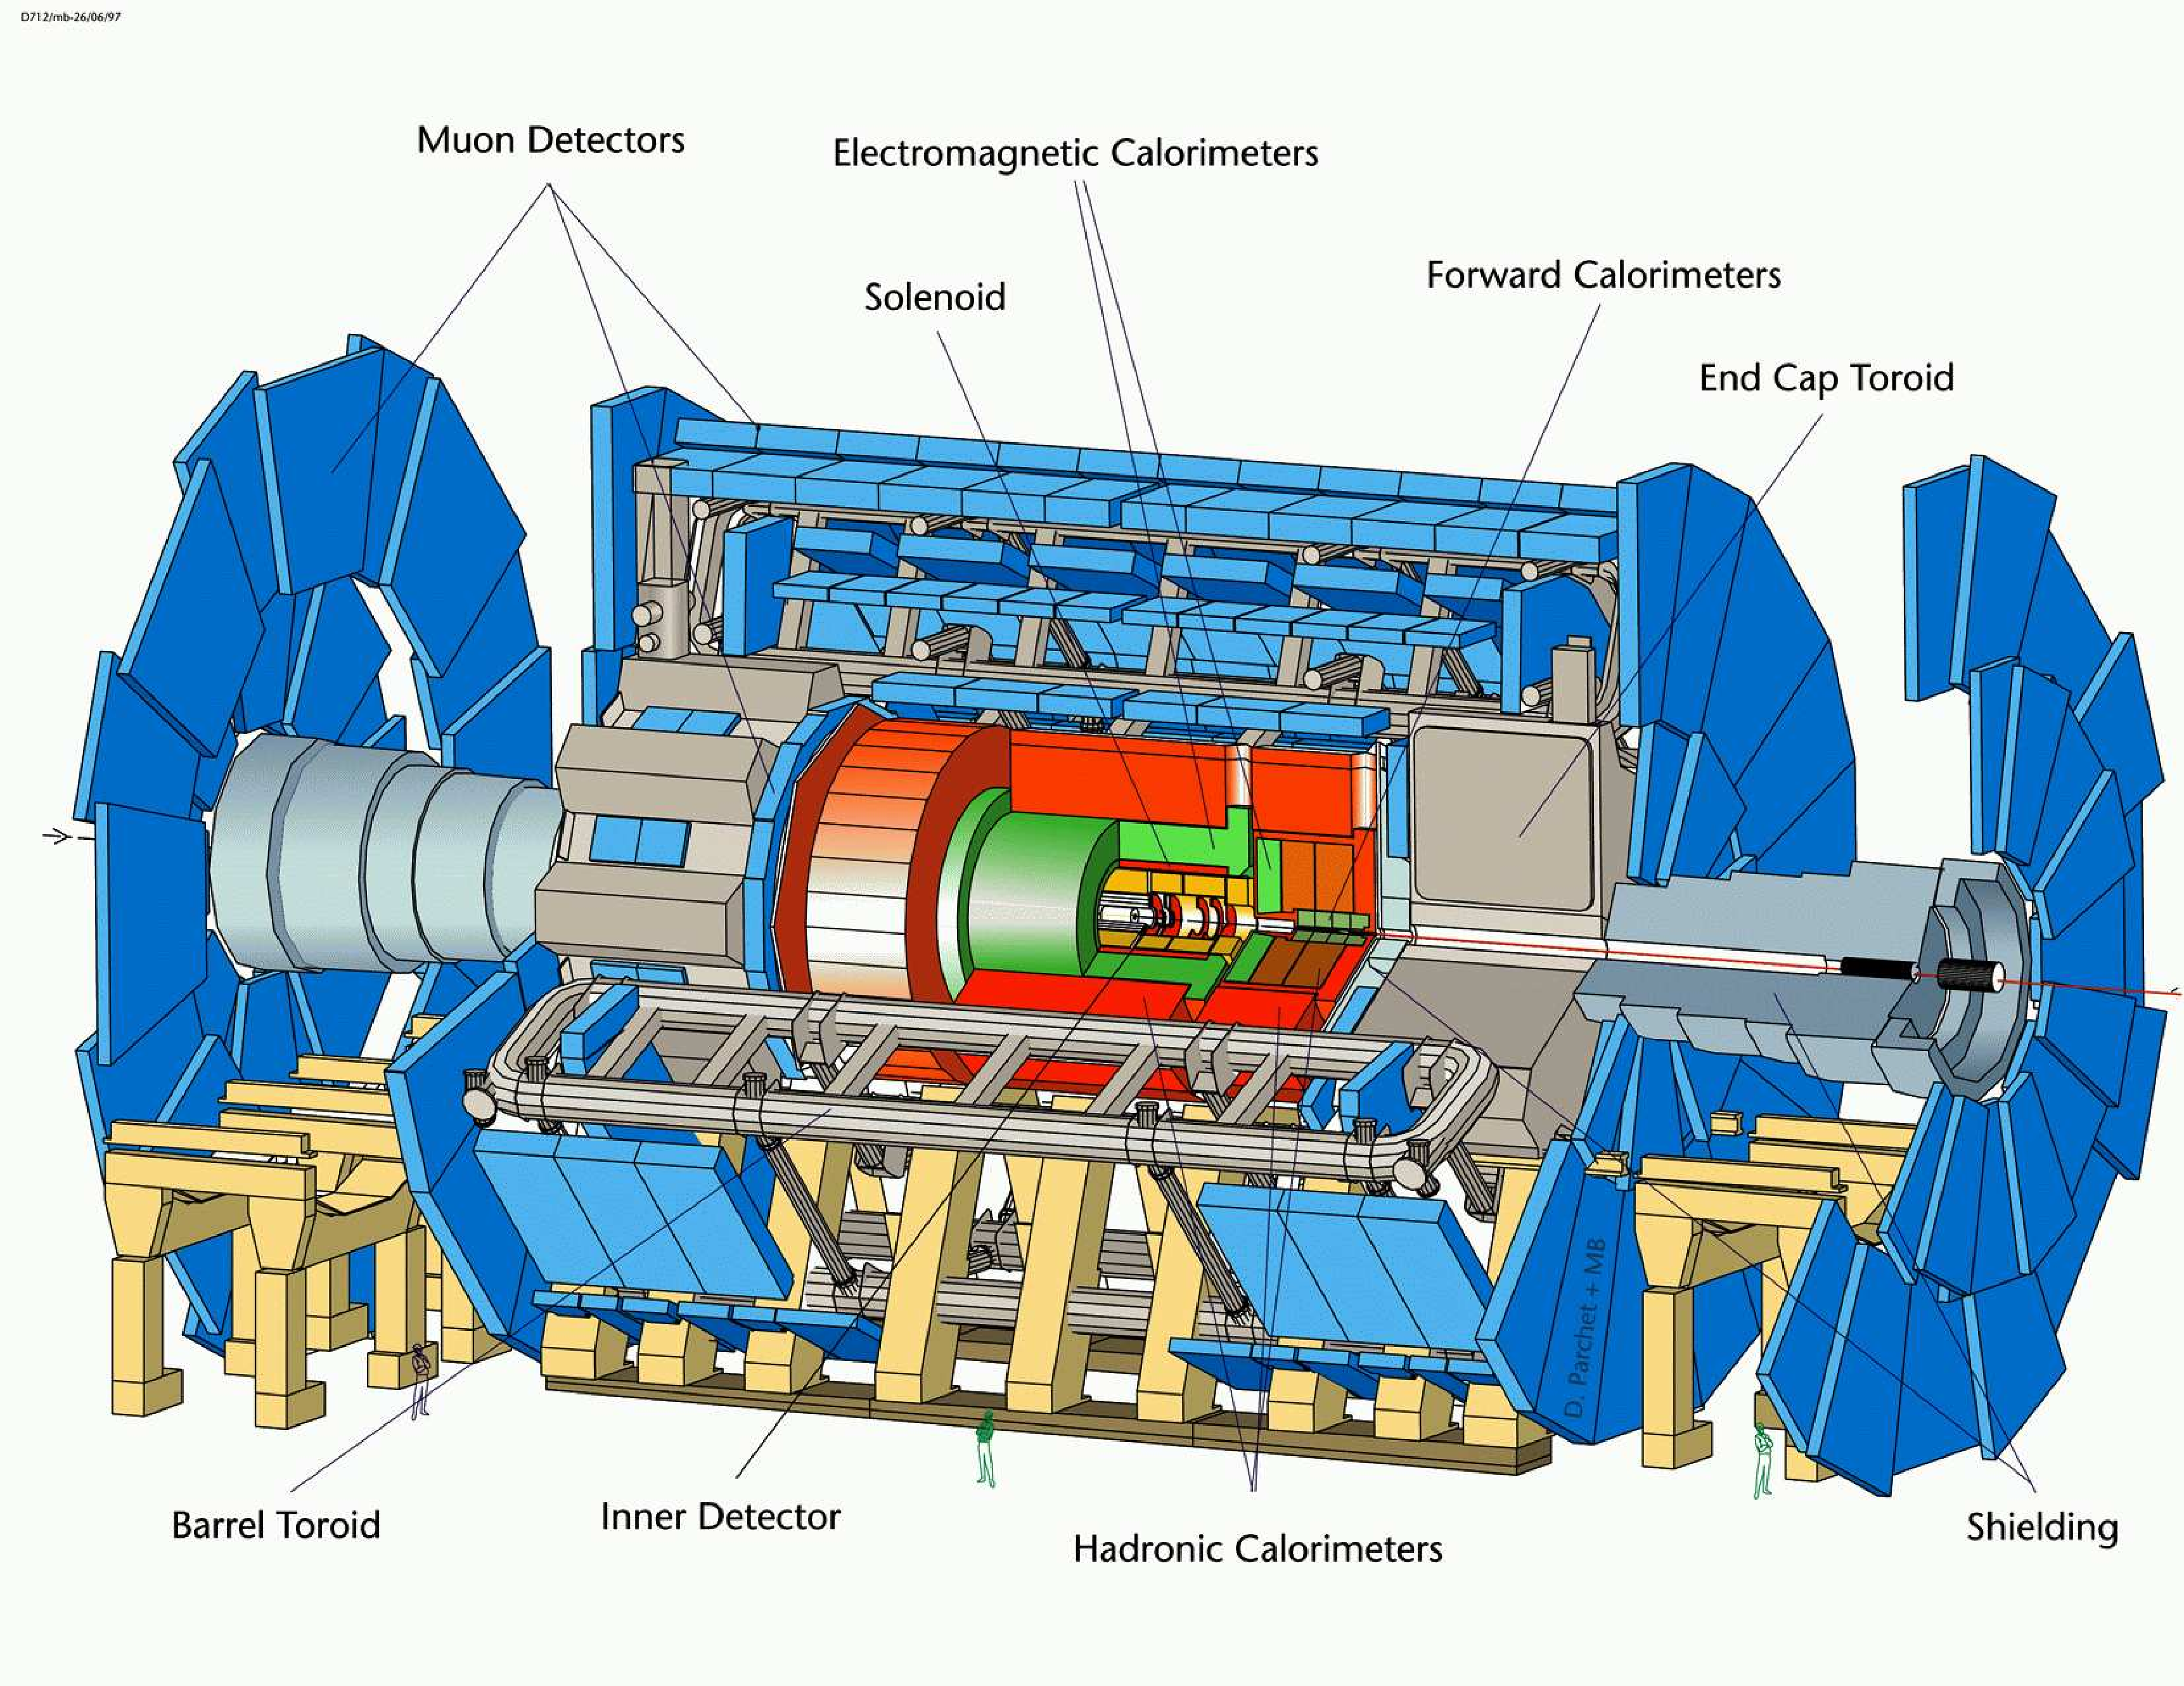
\includegraphics[width=\textwidth]{Diagrams/atlas.eps}
\caption[The ATLAS Detector]{The ATLAS detector \cite{:1999fq}.\label{ATLAS}}
\end{figure}

\subsection{The Inner Detector}

The ID \cite{:1999fq:Chapter1,:1999fq:Chapter3} comprises three sub-detectors covering the pseudo-rapidity range $|\eta| < 2.5$. 
%and is shown in figure \ref{InnerDetector}.  
 The detector nearest the beam is the pixel detector, which is surrounded by the semi-conductor tracker (SCT). The outermost detector is the transition radiation tracker (TRT). Each of these sub-detectors is split into three main components. One is a barrel region which is cylindrical about the beam line with the interaction point at the centre. The other two are endcap regions either side of the interaction point.

%The pixel detector and the SCT are made from silicon. A charged particle passing through the silicon creates electron-hole pairs and a bias voltage across the silicon causes the charges to drift to a readout. If the amount of charge produced is greater than a threshold value then a particle hit is recorded. The TRT is based on straw detector technology. The straws are filled with gas, and a particle traversing the gas causes ionisation. The electrons drift toward a wire readout in the centre of the straw, due to a bias voltage. A particle hit is defined in a similar way to the silicon detectors using a threshold of collected charge.

The pixel detector and the SCT are made from silicon. A charged particle passing through the silicon creates electron-hole pairs and a bias voltage across the silicon causes the charges to drift to a readout electrode. If the amount of charge produced is greater than a threshold value then a particle hit is recorded.
% The pixel detector 

The pixel detector is granular and segmented into pixels of 50~$\mu$m~$\times~$300~$\mu$m. A pixel module consists of 61440 pixels in a 21.4~mm~$\times$~62.4~mm rectangle. In the barrel region, the longer edge of each module is aligned in the $z$ direction and the shorter edge in $R_{\phi}$. The barrel consists of three layers of modules, with each layer providing coverage of $|\eta| < 1.7$ and complete coverage in azimuth. The granularity of the pixels allows precise measurements in $R_{\phi}$ and $z$, with a resolution of 12~$\mu$m and 66~$\mu$m respectively.
%The barrel layers cover the radial region of 4-11cm from the beam. 
Each pixel end-cap consists of five disks of modules covering the pseudo-rapidity range $1.7<|\eta|<2.5$. The position resolution is 12~$\mu$m in $R_{\phi}$ and 77~$\mu$m in $R$.

%The resolution in the position measurement of the pixel detector is 12$\times$66$\mu$m in barrel and 12$\times$77$\mu$m in the end cap disks.
%pixel based on silicon semi conductor technology. charged particle passing through causes electron hole pairs in the semi conductor. A voltage bias collects the charge.
%pixels are segmented in rphi and z.
% individual pixel is 50um x 300um in rphi,z. A module 21.4x62.4mm (61440 pixels). barrel (eta<1.7) has 3 layers, the first starting 4cm from the beam. 5-end cap disks (1.7<eta<2.5) - nearest 11cm radii from beam. The resolution in the measurement is 12x66um in barrel and 12x77um in the end cap disks.

% The silicon tracker
The SCT is made of single sided p-on-n silicon microstrip detectors which have dimension 6.36~$\times$~6.40 cm$^2$ (in the barrel region). Each detector consists of 768 strips of 80~$\mu$m pitch.
% In the barrel region ($|\eta|<$), 768 microstrips are combined into units of 6.36$\times$6.40cm. 
A module consists of four of these detectors, which are wire bonded in pairs to give a length of 12.8~cm. These pairs are then glued back to back at a crossing angle of 40~mrad. This allows precision measurement in one direction, using the granularity provided by the microstrip width, and another measurement perpendicular to the strips using small angle stereo. In the barrel ($|\eta|<1.4$), there are 4 layers of modules which are arranged so that the strips offer segmentation of the $R_{\phi}$ direction. This results in a resolution in $R_{\phi}$ of 16~$\mu$m and the small angle stereo gives a $z$ measurement accurate to 580~$\mu$m. 

The two SCT end-caps each consist of nine disks covering the range $1.4<|\eta|<2.5$. The end-cap modules are constructed in the same way as the barrel modules. However, the microstrips themselves are tapered and there are three sizes of module covering the inner, middle and outer regions of the disk. The modules are aligned on the disks so that one set of strips is in the radial direction, again giving precision measurements in the $R_{\phi}$ direction. The resolution of the end-cap measurements in ($R_{\phi}$, $R$) is the same as the barrel measurements in ($R_{\phi}, z$).
%  barrel : 4 layers of modules. end-cap is 9 disks of modules. Each module has 2 p on n silicon microstrip detectors at a crossing angle of 40mrad. In barrel, each detector is 6.36x6.40cm with 768 strips of 80um pitch. precision measurements in the Rphi direction gives 16um resolution. Small angle stereo gives the z measurement to a resolution of 580um. Are we sure how the small angle stereo works?
% The TRT

The TRT is based on straw detector technology. The straws are filled with gas (70\% Xe, 27\% CO$_2$, 3\% O$_2$) and a charged particle traversing the gas causes ionisation. The electrons drift toward a wire readout in the centre of the straw, due to a bias voltage. A particle hit is defined in a similar way to the silicon detectors using a threshold of collected charge.
The TRT is made of straws 4~mm in diameter and up to 144~cm long. The barrel section ($|\eta|<0.7|$) has 50000 straws, aligned lengthways in the $z$ direction. The end-cap wheels have 320000 radial straws, which are arranged in 18 wheels per end-cap and cover the pseudo-rapidity region $0.7<|\eta|<2.5$. Drift time measurements result in a resolution of 170~$\mu$m per straw. A charged particle passing through the TRT gives typically 36 hits per track.

Radiator material is placed between the straws. Particles with $\beta\gamma \geq 1000$ emit transition radiation photons at the radiator-straw boundary. The emitted radiation is absorbed by the xenon and results in more ionisation than just the initial particle alone. The TRT uses a second, higher threshold to determine whether the hit consists of a particle plus transition radiation. This mechanism allows electron-pion separation in the momentum range $p < 100$~GeV. 

 %because electrons emit transition radiation and pions do not. 
% Above this $p_{T} limit$, the rise of ionisation with $B^2$ causes the separation
%stuff here on trans rad
%i have no idea how this works.
%As electrons traverse the TRT, they emit transition radiation as they pass between straws. The gas mixture in the straws contains Xenon, which is ionised by the transition radiation photons. A second thres

%straw detectors-
%particles ionise the gas to form electron ion pairs. A bias voltage causes the electrons to drift to a sense wire. Each straw is 4mm in diameter and 144cm long with 30um sense wire. Each straw is divided into 2 at centre to reduce occupancy. barrel has 50000 straws. end cap 320000 radial straws arranged in 18 wheels in each cap. Drift time measurement results in resolution of 170um per straw.
%typically 36 hits per track at LHC
%TRT also gives some electron id by detecting photons created as electrons travel through straw-gap-straw boundaries.
%the magnet effects.

The ID is surrounded by a superconducting central solenoid magnet which provides a 2~T magnetic field in the $z$ direction. The central solenoid is kept at 4.5~K and shares the same vacuum vessel as the electromagnetic barrel calorimeter. The charged particles bend in the presence of the magnetic field and the transverse momentum of the particle can be obtained from the radius of curvature of the track. The large number of track hits in the TRT, coupled with the precision measurements of the silicon detectors, result in excellent reconstruction of particle pseudo-rapidity, azimuth, impact parameter ($d_0$) and vertex identification ($z_0$). The resolution of reconstructed muon track parameters, obtained from full simulation \cite{:1999fq:Chapter3}, are:
\begin{eqnarray} \label{trackrec}
\sigma\left(\frac{1}{p_T} \right) & = & 0.36 + \frac{13}{p_T\sqrt{\sin\theta}} \quad(\text{TeV}^{-1})  \nonumber \\
%\qquad 
\sigma\left(\phi \right) & = & 0.075 + \frac{1.8}{p_T\sqrt{\sin\theta}} \quad(\text{mrad}) \nonumber \\
%\nonumber
%\vspace{0.1cm}
%\end{equation*}
%\begin{equation*}
\sigma\left(\cot\theta\right) & = &  \left(0.7 +  \frac{2.0}{p_T\sqrt{\sin^{3}\theta}}\right)\times10^{-3} \nonumber \\
%\qquad
\sigma\left(d_0\right) & = & 11 + \frac{73}{p_T\sqrt{\sin\theta}} \quad (\mu\text{m}) \nonumber \\
%\vspace{0.1cm}
%\end{equation*}
%\begin{equation}\label{trackrec}
\sigma\left(z_0\right) & = & 87 + \frac{115}{p_T\sqrt{\sin^3\theta}} \quad (\mu\text{m}).
%\vspace{0.1cm}
\end{eqnarray}
Pions and electrons are less well measured. Pions have a probability of undergoing a nuclear interaction, which causes tails in reconstructed track parameters. This problem is removed by the standard track quality cuts which are \cite{:1999fq:Chapter3}: at least nine precision hits in the silicon detectors, at least two pixel hits - with one in the inner layer - and a transverse impact parameter less than 1~mm.  The effect of these track quality requirements is to reduce the efficiency of pion track reconstruction, but results in similar resolutions as equation \ref{trackrec}. Electrons on the other hand, emit bremsstrahlung
radiation which leads to a broadening of the smeared distributions of 1/$p_T$, $d_0$ and $\phi$.

\subsection{The Calorimeters}

Calorimeters measure the total energy of particles by complete absorption. The two ATLAS calorimeters \cite{:1999fq:Chapter1,:1999fq:Chapter4,:1999fq:Chapter5} use alternating sheets of material to repeatedly sample the energy. The first type of material causes the particles to shower into a number of secondary particles. The second type of material forms the active part of the detector, which absorbs and measures some of the energy of the produced particles. This process is repeated in many layers until all of the energy is absorbed. 
% differnce in types of showers. - allow differnt calorimeters..shower shapes.

The electromagnetic calorimeter (EM) uses a lead/liquid argon combination to measure the energy of photons and electrons. In the presence of heavy nuclei, electrons emit bremsstralung photons; photons on the other hand split into an electron-positron pair. Thus an incident electron or photon results in a shower of new particles when passing through the lead layer.
%Lead is used in this process due to a high atomic number which results in a short radiation length. 
The electrons produced in the shower cause ionisation in the liquid argon (LAr) and the charge is collected on copper electrodes.

The barrel EM calorimeter covers the region $|\eta|<1.475$ and the end-caps cover $1.375 < |\eta| < 3.2$. However, in the pseudo-rapidity region $|\eta| < 1.8$, the EM calorimeter is preceded by a presampler, which is a just a layer of liquid argon (LAr). The reason for this is that the material preceding the calorimeter can cause showering and the presampler corrects for this energy loss. 

The EM barrel calorimeter is split into three sampling regions of differing granularity that are arranged in layers. The inner layer has a granularity of 0.003~$\times$~0.01 in $\eta\times\phi$ and a depth of
approximately six radiation lengths.
% 4.3 radiation lengths.
The second sampler absorbs the majority of the energy of the particle due to a radial depth of more than 16 radiation lengths and has a granularity of 0.025 in both $\eta$ and $\phi$. The final layer is coarser, with a granularity of 0.05~$\times$~0.025 in $\eta\times\phi$, and is between 2 and 12 radiation lengths in depth. The EM end-caps have a more complicated geometry, shown in table \ref{EMendcap}, where the granularity and number of samplings depends on the pseudo-rapidity. The end-caps are more than 26 radiation lengths in depth.

The energy resolution, $\sigma_E$, of the EM calorimeter is parameterised  by
\begin{equation}\label{Ecalres}
\frac{\sigma_E}{E}=\sqrt{\left( \frac{a^2}{E} + b^2\right)}
\end{equation}
where 
%E is the energy of the particle, 
$a$ is a sampling term (\%~GeV$^{1/2}$) and $b$ is a constant  ($\%$). The  sampling term varies between 8 and 13 from low to high rapidity when a full simulation of the calorimeter is used \cite{:1999fq:Chapter4}. The constant term is less than 0.5$\%$ for electrons and less than 0.25$\%$ for photons.

\begin{table}[htdp]
\begin{center}
\begin{tabular}{|c|c|c|c|}
\hline
End-Cap & Sampling number & $|\eta|$ & $\eta\times\phi$ \\
\hline
EM & 1 & 1.375 $< |\eta| <$ 1.5 & 0.025$\times$0.1\\
 & & 1.5 $< |\eta| <$ 1.8 & 0.003$\times$0.1 \\
 & & 1.8 $< |\eta| <$ 2.0 & 0.004$\times$0.1\\
 & & 2.0 $< |\eta| <$ 2.5 & 0.006$\times$0.1\\
 & & 2.5 $< |\eta| <$ 3.2 & 0.1$\times$0.1\\
 & 2 & 1.375 $< |\eta| <$ 2.5 & 0.025$\times$0.025\\
 & & 2.5 $< |\eta| <$ 3.2 & 0.1$\times$0.1\\
 & 3 & 1.5 $< |\eta| <$ 2.5 & 0.05$\times$0.025\\
 \hline
HEC & All & 1.5 $< |\eta| <$ 2.5 & 0.1$\times$0.1\\
 & All & 2.5 $< |\eta| <$ 3.2 & 0.2$\times$0.2\\
\hline
\end{tabular}
\end{center}
\caption[The granularity ($\eta\times\phi$) of the end-cap calorimeters]{The granularity ($\eta\times\phi$) of the electromagnetic (EM) and hadronic (HEC) end-cap calorimeters \cite{:1999fq:Chapter1}.}
\label{EMendcap}
\end{table}%

%Interaction of hadrons - no do it later
%
%

The hadronic calorimeters are used to measure the energy of baryons and mesons. 
In the barrel ($|\eta|<1.0$) and extended barrel ($0.8<\eta<1.7$) regions, iron is used to shower the hadrons and 3~mm scintillating tiles are used as the active absorber. Each side of the tile is read out by a photomultiplier tube. The readout cells are divided to give 64 modules in azimuth. In the $z$ direction, the readout from the cells are grouped in such a way so that the resulting granularity is 0.1~$\times$~0.1 in $\eta\times\phi$ for the first 2 samplings. The final sampling is less granular with $\eta\times\phi = 0.2\times0.1$.

The hadronic end-cap, $1.7<\eta<3.2$, is split into two wheels and uses copper to provide the hadron shower and an 8.5~mm LAr gap as the active absorber. There a four sampling regions and the granularity   depends on the pseudo-rapidity as in the EM end-cap. The granularity is given in table \ref{EMendcap}. 
The forward calorimeter, $3.1<\eta<4.9$, also uses liquid argon and consists of three sections. Each section consists of a metal matrix (copper or tungsten) with regularly spaced channels. Cylindrical rods are placed in the channels and carry high voltage, which causes the charge drift in the LAr gap. The resulting granularity is $\eta\times\phi=0.2\times0.2$.

The resolution in energy measurement for hadrons takes into account energy deposited in the EM and hadronic calorimeters and also dead material in the detector. The resolution is parameterised \cite{:1999fq:Chapter5} by
\begin{equation}
\frac{\sigma_E}{E} = \frac{A}{\sqrt{E}} + B
\end{equation}
where $A$ and $B$ are the sampling and constant terms respectively. The sampling and constant terms for pions, obtained from full simulation, are pseudo-rapidity dependent and are given in table \ref{hadronres}.

\begin{table}[t]
\begin{center}
\begin{tabular}{|c|c|c|}
\hline
$|\eta|$ & $A$ \small{(\%GeV$^{1/2}$)} & $B$ ($\%$) \\
\hline
0.3 & 40$\pm$1 & 3.0 $\pm$ 0.1 \\
1.3 & 44$\pm$3 & 1.6 $\pm$ 0.3\\
1.8 $< |\eta| <$ 3.05 & 55 $< A <$ 60 & 2.5 $< B <$ 3.0 \\
\hline
\end{tabular}
\end{center}
\caption[The sampling and constant terms for pion energy resolution.]{The sampling ($A$) and constant ($B$) terms for pions. The final resolution combines information from the electromagnetic and hadronic calorimeters and corrects for energy lost in dead material such as the cryostat wall \cite{:1999fq:Chapter5}.}
\label{hadronres}
\end{table}%

\subsection{The Muon Spectrometer}

The muon spectrometer \cite{:1999fq:Chapter1,:1999fq:Chapter6} is designed to determine the transverse momentum and charge sign of muons by measuring the radius of curvature of muon tracks in a magnetic field. The magnetic field is provided by three superconducting air-core toroid systems (shown in figure \ref{ATLAS}). 
The end-cap toroids are inserted into the barrel toroid. The overall bending power is 2-6~Tm in the pseudo-rapidity region $|\eta|<1.3$ and 4-8~Tm in the region $1.6<|\eta|<2.7$. The overlap region of the barrel and end-cap toroids, $1.3<|\eta|<1.6$, has a lower bending power.

The muon spectrometer is divided into precision tracking and trigger chambers. In the barrel region, $|\eta|<1.0$, the precision chambers are arranged into three stations of monitored drift tubes (MDTs). The MDTs are made from 30~mm aluminium tubes, each with a 50~$\mu$m W-Re readout wire in the centre. %The tubes are between 70cm and 630cm in length. 
The single wire resolution is 80~$\mu$m. A super-layer is defined as four layers of tubes in the inner station and three layers in the middle and outer stations. The chambers themselves consist of two super-layers, one on each side of the support structure to which they are attached. The barrel muon spectrometer consists of 1194 such chambers.

In the end-caps, the precision chambers are MDTs in the region $1.0<|\eta|<2.0$ and cathode strip chambers (CSCs) in the region $2.0<|\eta|<2.7$. The CSCs are multi-wire proportional chambers with the first set of cathode strips perpendicular to the anode. The precision point is measured by reading out the induced charge on the cathode due to electron avalanche on the anode. The second set of cathode strips is parallel to the anode and thus provides the transverse component. The position resolution of the cathode strips is 60~$\mu$m.

The momentum resolution of the muon spectrometer depends on the transverse momentum and pseudo-rapidity of the muon itself. High transverse momentum muons are bent less in the magnetic field and hence the radius of curvature is less well measured. In the overlap region between barrel and end-cap toroids, the bending power is smaller and hence the momentum less well measured. Even so, the momentum resolution of the muon spectrometers, for more than 75\% of the available phase space, is approximately $3\%$ for muons with 30~GeV$ < p_T < 100$~GeV, better than $5\%$ for $p_T<300$~GeV  and approximately $10\%$ for 1~TeV muons \cite{:1999fq:Chapter6}. 

The trigger chambers are resistive plate chambers (RPCs) in the barrel region, $|\eta|<1.0$, and thin gap chambers (TGCs) in the region $1.0<|\eta|<2.4$. An RPC unit is made of two parallel resistive plates separated by a gas gap. Each trigger chamber consists of two such units and the resolution in space-time of the RPCs is approximately 1~cm~$\times$~1~ns. The ionisation electrons are multiplied by an electric field of 4.5~kV~mm$^{-1}$ and the resultant charge is read out by perpendicular sets of metal strips on either side of the unit. The $\eta$ strips are aligned with the wires in the MDTs. The $\phi$ strips are then used in offline reconstruction. The TGCs are multi-wire proportional chambers with a gas gap of 2.8~mm and a wire pitch of 1.8~mm. The wires are aligned with the wires in the MDTs. Graphite cathode read-out strips, which are arranged perpendicular to the anode wires, fan out radially from the beampipe and provide the azimuthal coordinate in offline reconstruction. 

\subsection{Trigger and Data Acquisition} \label{triggers}

It is not desirable for the ATLAS collaboration to store all the event data from every bunch crossing. Firstly, each event will occupy approximately 1.5~MB of memory in offline storage. As the bunch crossing rate at the LHC will be 40~MHz, this would correspond to a data rate of 60~TB~s$^{-1}$. Secondly, the majority of these events will be soft QCD events. New physics signals, such as the discovery of the Higgs boson, will be relatively rare and searching through such a large data set for a potential signal would take too long. A better strategy therefore, would be to examine the data immediately and store the event permanently only if it passes a set of criteria. This is known as triggering.

The ATLAS trigger \cite{:1999fq:Chapter1,:1999fq:Chapter11} is designed to execute in three successive stages; level 1, level 2 and the event filter. 
For each bunch crossing, the information from each sub-detector is pushed into pipeline memories. Each sub-detector then identifies which memory block corresponded to a particular bunch crossing after receiving a clock signal from the level 1 central processor. For practical and economical reasons the length of the pipelines must be kept short and this limits the time the sub-detector will retain the information.

The level 1 trigger has the initial responsibility of retaining events of possible interest. The decision to keep an event is made within 2.5~$\mu$s. The trigger relies on reduced granularity information from the muon spectrometer and calorimeters in order to define objects of interest. Muons are identified using just the RPCs and TGCs. The calorimeter trigger is used to define electron/photon, tau, jet, missing and scalar transverse energy objects. 
%For each level 1 object, there are a number of thresholds that can be passed as shown in figure \ref{level1objects}. 

A physics menu provides a list of criteria that define objects of potential interest. An example of a level 1 physics menu is shown in table \ref{menulvl1}. The jet triggers have a very high transverse energy threshold because of the very large QCD rate at low transverse energy. The muon transverse momentum requirement is low in order to keep soft muons from B-physics events. If an object passes one of these criteria, the entire event is kept. The data is then read out, formatted and stored in read-out buffers (RoBs).
The maximum data rate of events selected at level 1 is 75~kHz. The current estimate, given in table \ref{menulvl1}, is 44~kHz.
%%talk about jets at level 1????

\begin{table}[t]
\centering
\begin{tabular}{|c|c|}
\hline
Trigger & Rate (kHz) \\
\hline
MU6 & 23\\
EM20I& 11\\
EM15I $\times2$& 2\\
J180 & 0.2\\
J75 $\times$3 & 0.2\\
J55 $\times$4 & 0.2\\
J50 + XE50& 0.4\\
T20 + XE30 & 2\\
Other & 5\\ 
\hline
\end{tabular}
\caption[ATLAS low luminosity level 1 trigger menu]{Low luminosity level 1 trigger menu \cite{:1999fq:Chapter11} with expected trigger rates. The following codes are standard in level 1: MU(muon spectrometer), EM(electromagnetic object), J(jet), T(tau), XE(missing $E_T$) and I is an isolation criterion. For example, EM20I means the (reduced granularity) electromagnetic object must have an $E_T > 20$~GeV and be isolated from other EM activity.\label{menulvl1}}
\end{table}%

The level 2 trigger operates on regions-of-interest (RoIs). An RoI is a small amount of information provided by level 1 that allows level 2 to request read-out data from relevant sub-detectors, i.e those near the region of interest. Level 2 starts out by confirming the level 1 result. The level 2 trigger then refines the result by searching other sub-detectors for relevant information. In the case of muons for example, an isolation criterion can be applied by looking for activity in the calorimeters. Level 2 then defines global trigger objects based on information from all sub-detectors and makes a decision to keep the event or not. The total processing time at level 2 is approximately 10~ms and the data rate which is passed to the event filter is approximately 2~kHz.
The event filter further refines the event by using the full granularity of the detector. It is at this stage that the most complex algorithms, such as track fitting or vertex reconstruction, are applied to the data because the processing time is a few seconds. The final event rate is expected to be approximately 100~Hz.



\section{The FP420 Project} \label{fp420}

FP420 is a proposed new sub-detector capable of measuring the momenta of the protons scattered in central exclusive processes \cite{Cox:2005tb}. The basic design of FP420 is a magnetic spectrometer. The protons scattered during the interaction will have lower momentum than the beam protons and will be bent out of the beam by the superconducting magnets in the LHC ring. The aim is to install movable silicon tracking detectors 420~m either side of the interaction point. The measurement of the angle and displacement of the protons with respect to the beam line will allow the proton momentum to be determined if the beam optics are well known.%large dispersion at 420

In the present design of the LHC, there is a 15~m connection cryostat in the 420~m region. The cross section of the cryostat is shown in figure \ref{cryostat420}. V1 and V2 are the beam pipes, with V2 containing the outgoing beam from the interaction point. The detector stations will be placed between V1 and V2. M1, M2 and M3 are superconducting bus bars which carry the current for the magnets. It is possible to move these bus bars to make extra room for detector access. 
%A possible re-design of the cryostat region is shown in figure \ref{cryostat420} (b). The region marked XX would contain the bus bars. 
The heat exchanger, labelled $X$, cannot be moved because it must remain parallel to the tunnel floor at all times. 
%this bit is about the cold bit.......do i need it?
%The 420m region is a `cold' region which means that the beam pipes are at 1.9K. The FP420 design will, point::::::> no longer a cryo!!!!!!

\begin{figure} [t]
\centering
    	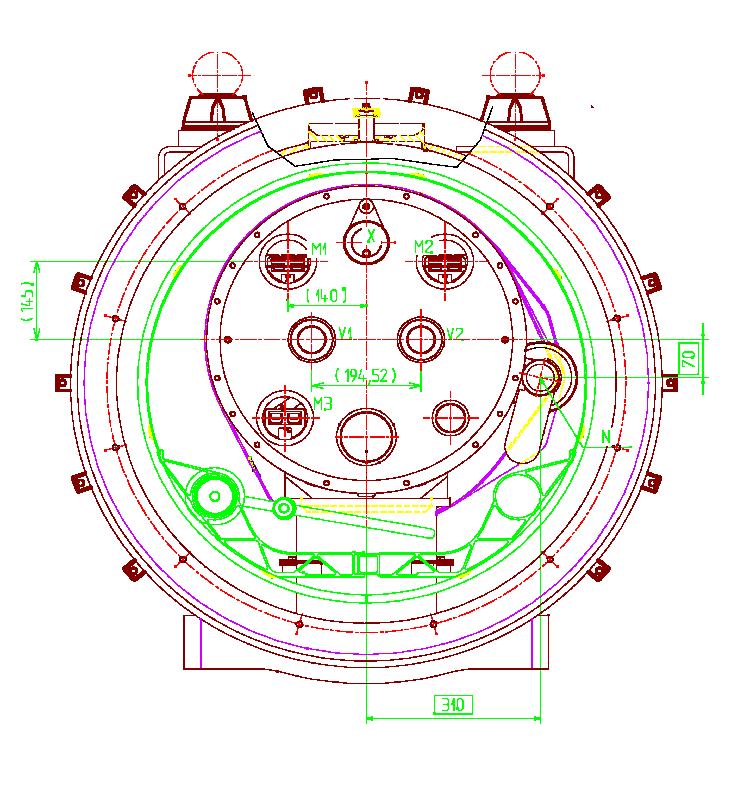
\includegraphics[width=0.65\textwidth]{Diagrams/Cryostat.eps}
\caption[The 15~m cryostat at 420~m from the ATLAS interaction point]{The 15~m cryostat at 420~m from the ATLAS interaction point \cite{Cox:2005tb}.\label{cryostat420}}
\end{figure}

%check this next bit %prev say that two sets of detectors 8m apart ??
The detector stations will be moved closer to the beam after proton injection and acceleration, when the beam has stabilised. 
%delete this if incorrect.........
The Hamburg Pipe design proposes that the stations will be rigidly fixed to the V2 beam pipe and the position measured to 1~$\mu$m with an optical bench arrangement. The entire structure will then be moved to place the detectors closer to the beam line itself. 
%
%
The position of each station with respect to the beam will be measured using beam positioning monitors (BPMs), which are precise to a few 10's of $\mu$m. %A greater precision can be achieved using a known high-rate process 
At least two detector stations will be required to make the momentum measurement, but 3-4 could be used for redundancy purposes and background (halo) rejection. The stations will be placed over an 8~m length along the beam pipe.

%some citations needed here.......
Each detector station will be capable of measuring the position of the proton relative to the beam and the time of flight (TOF) of the proton from the interaction point.
The position measurement will be made using layers of 3D edgeless silicon. It is estimated that the position of a proton hit within the silicon layers can be measured to 10~$\mu$m and the angle to 1-2 mrad \cite{Cox:2005tb}. The limiting factor on the relative position measurement will be due to the BPMs and this can probably be improved using clean high rate processes such as $\gamma \gamma \rightarrow \mu^{+} \mu^{-}$ in off-line calibration.

The TOF detectors will be fast-timing Cerenkov counters. Protons traversing the active volume will emit Cerenkov radiation which is then detected by photo-multiplier tubes. Two types of TOF unit will be used; GASTOF and QUARTIC, which are designed to use gas and quartz respectively. GASTOF will be used in the stations nearest the interaction point whilst QUARTIC will be used only in the final station and will be positioned after the silicon layers. This configuration was chosen because there will be a large probability for the proton to have multiple scatterings in  quartz, which could change the direction of the proton or cause it to break up completely. Thus QUARTIC can only be used after all of the position measurements.
The final TOF measurement is estimated to be accurate to 10~ps. The TOF measurements for the outgoing protons either side of the interaction point will be made relative to each other, making a reference clock unnecessary. The $\Delta$TOF measurement
corresponds to an interaction vertex measurement with an accuracy of 2.1~mm.

The $\xi$ acceptance will depend upon how close the detector stations can get to the beam and the dispersion of the LHC at 420~m. The closest distance of approach to the beam has been considered to be 10$\sigma_x + 0.5$~mm \cite{Alekhin:2005dy:TOTEM},
where $\sigma_x$ is the horizontal beam width at 420~m. This results in a lower limit of 3~mm and will require ideal beam conditions. Larger distances of 5~mm, 7.5~mm and 10~mm have also been studied \cite{Cox:2005tb}. The distance from the beam will affect the low $\xi$ acceptance, and hence the lower central mass reach of FP420. However, using the FPTRACK program \cite{PeterBusseyAcceptance}, it was found that the acceptance for a 120~GeV central mass is constant for the three closest configurations as shown in figure \ref{fp420accept}. The $\xi$ acceptance of the 5~mm configuration is given \cite{PeterBusseyAcceptance} by %PB
\begin{eqnarray}
0.0023 & \leq \xi_1 \leq & 0.0129 \nonumber \\
0.0029 & \leq \xi_2 \leq & 0.0171 
\end{eqnarray}
where the asymmetry is due to differences in the beam optics on each side of the ATLAS detector. The dominant contribution to the uncertainty in the momentum loss measurement is expected to be the intrinsic momentum spread of the protons within the beam at the LHC (0.77~GeV). This is also the dominant uncertainty on the resolution on the central mass measurement, which is estimated to be $1-2\%$. 

\begin{figure} [t]
\centering
    	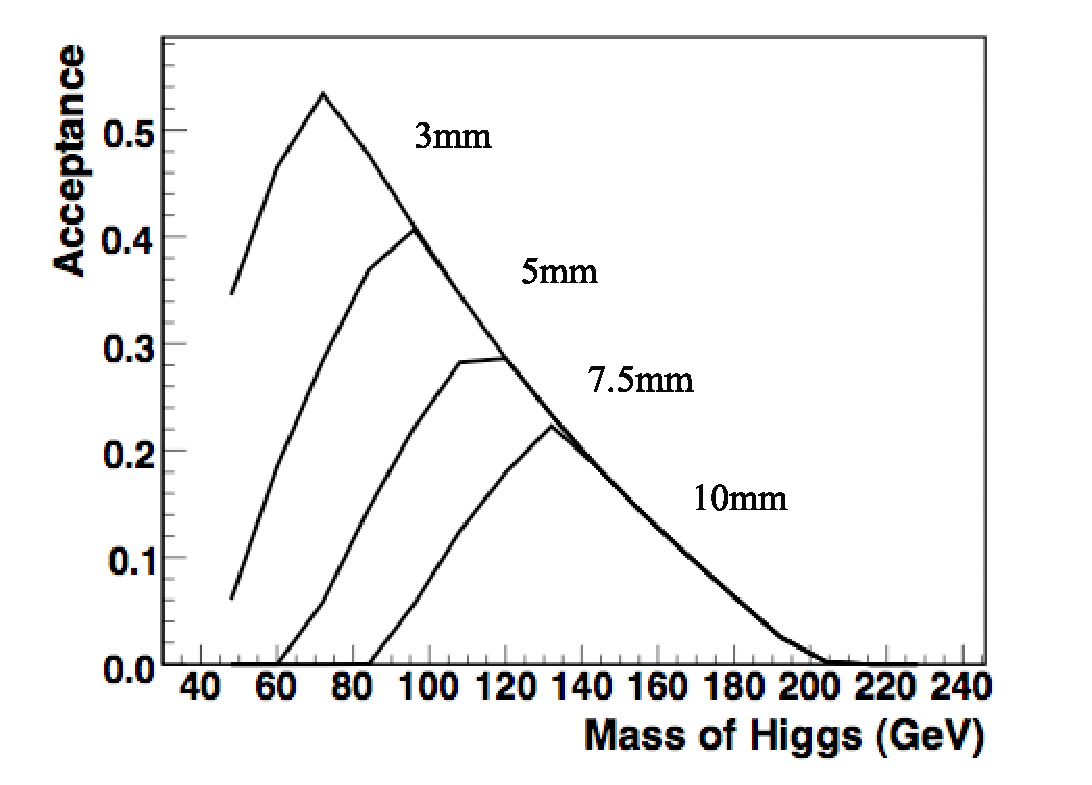
\includegraphics[width=0.65\textwidth]{Diagrams/peterbusseyacceptance.eps}
\caption[The acceptance of FP420 as a function of the mass of the central system]{The acceptance of FP420 \cite{Cox:2005tb} as a function of the mass of the central system. Results are shown for different distances of closest approach to the beam.\label{fp420accept}}
\end{figure}

Finally, the signal from FP420 will arrive at the central trigger processor 3~$\mu$s after the interaction occurred. This means that information from FP420  can only be used at trigger level 2 onwards. Thus the central exclusive events will only be available for analysis if they pass one of the standard level 1 triggers given in section \ref{triggers}.


\chapter{The ExHuME Generator}
\section{Monte Carlo Methods} \label{mcmethods}

\subsection{Monte Carlo Integration}

The basic Monte Carlo (MC) method is an integration technique based on randomly sampling a distribution. Consider a one dimensional function, $f(x)$. The definite integral, $I$, can be estimated \cite{Langanke:1993qn} by 
\begin{equation} \label{onedint}
I = \int^{x_{2}}_{x_{1}} f(x) dx \approx \frac{x_{2}-x_{1}}{N} \sum_{i=1}^{N} f(x_i)
\end{equation} 
where $N$ is the number of sampling points chosen randomly in the range $\{x_{1}, x_{2}\}$. The function is averaged across the specified range and the approximation becomes exact as $N\rightarrow\infty$. The uncertainty in the integral, $\sigma_I$, is calculated by
\begin{equation}\label{onederror}
\sigma_{I}^2  = \frac{\left(x_2 - x_1\right)^2}{N}\left[\frac{1}{N}\sum_{i=1}^{N} f(x_i)^2 - \left(\frac{1}{N}\sum_{i=1}^{N}f(x_i)\right)^2 \right]
\end{equation}
where the term in square brackets is the variance of the function.
The uncertainty in the integral can be reduced significantly in two ways. Firstly, the uncertainty  decreases with $N^{1/2}$, which means that sampling more points results in a better estimate of the integral. Secondly, the uncertainty decreases with the variance of the function. Therefore, if the amount by which a function varies from its average is reduced, the uncertainty in the integral will also decrease.

The smoothing out of functions in this way is achieved by the use of a weight function. A new integration variable, $y$, is introduced such that
\begin{equation}\label{changeintvar}
\frac{dy}{dx} = w(x)
\end{equation}
where $w(x)$ is the weight function.
%\begin{equation}
%\int_{x_{min}}^{x_{max}} w(x) dx = 1.
%\end{equation}
The integral can then be rewritten as 
\begin{equation}\label{ndint}
I = \int^{y_{2}}_{y_{1}} \frac{f(x(y))}{w(x(y))} dy \approx \frac{y_{2} - y_{1}}{N} \sum_{i=1}^{N} \frac{f(x(y_i))}{w(x(y_i))}
\end{equation}
 where the sampling points are chosen randomly in the range $\{y_{1}, y_{2}\}$. The uncertainty in the integral can be evaluated using equation \ref{onederror} with the substitution $f(x)\rightarrow\frac{f(x)}{w(x)}$. The uncertainty is now dependent on the variance of $\frac{f(x)}{w(x)}$, which can be minimised by an appropriately chosen weight function. 
 
The power of the MC integration technique is realised with the extension to an arbitrary number of dimensions. Each component of the $n$-dimensional point $\textbf{x}=(x^1,...,x^n)$ is chosen independently and the integral is approximated by
\begin{equation}
I \approx \frac{1}{N}\sum_{i=1}^{N} f(\textbf{x}_i) \prod_{j=1}^{n}\left( x^j_{2} -x^{j}_{1}\right) 
\end{equation}
where the product term is simply the volume element over which the integration is performed. An $n$-dimensional  weight function can then be chosen providing it factorises into the form
\begin{equation}
w(\textbf{x}) = \prod_{j=1}^{n} w(x^j) 
\end{equation}
where each $w(x^j)$ is a weight function for dimension $j$. This results in the new $n$-dimensional integration variable, $\textbf{y}$, the components of which are chosen randomly and  independently between $\{y^j_{1}, y^j_{2}\}$.


\subsection{Pseudo-Random Number Generators}

A computer does not generate true random numbers, but rather generates numbers according to an algorithm. These pseudo-random numbers appear random to someone who does not know the details of the algorithm. The generation of these numbers must have three important characteristics \cite{James:1988vf}. 

Firstly, the random number sequence must have a long period. Any algorithm that generates a sequence of numbers will eventually start repeating itself. For any given calculation, the number of pseudo-random numbers generated must not become close to the period of the sequence.

Secondly, the results of the generation must be repeatable. This is achieved by the use of a seed number from which the algorithm generates the sequence. Thus, the complete calculation can then be repeated and the same results obtained. The seed can also be recorded at any time. This allows a small subset of numbers to be recreated from a large sequence. This is desirable if, for example, a small set of numbers is changing the result of the calculation. The set can then be examined at any time without having to regenerate the  entire sequence.

The final requirement is a good distribution, which means that the random numbers should not be correlated and should be uniformly distributed. The only way to see if a random number generator results in a good distribution is to subject it to a variety of tests \cite{Vattulainen:1993rm,Rutti:2004th}. 

\subsection{Generation of Random Numbers to a Distribution}\label{mcdist}

The basic Monte Carlo evaluation of an integral required random numbers to be distributed uniformly in the integration variable of interest. The introduction of the weight function however, results in the random numbers being distributed uniformly in a new variable defined by equation \ref{changeintvar}. This can be viewed as the smoothing out of the function by changing integration variables. However, the uniform distribution of random numbers in this new variable is equivalent to the random numbers being picked - in the original integration variable - with a probability density defined by the (normalised) weight function. This is known as importance sampling because random numbers are more likely to be picked in regions of interest determined by the weight function.

This method only allows random numbers to be picked for an analytical function that is integrable. For a non-analytic function, Von~Neumann rejection can be used to distribute the random numbers. Von~Neumann rejection works as follows for a one dimensional function $f(x)$:
\begin{enumerate}
\item A weight function, $w(x)$, is chosen such that, for all $x$, $w(x) \geq f(x)$.
\item The random values of $x$ are distributed according to $w(x)$.
\item For each value of $x$, a random number, $r$, is picked in the interval $\{0, 1\}$.
\item The point is accepted if 
\begin{equation}
\frac{f(x)}{w(x)} \geq r .
\end{equation}
\end{enumerate}
The result of such an algorithm is shown in figure \ref{vonneu} (a). Using this method, random numbers can be distributed to any function providing a suitable weight function can be chosen. The efficiency, $\epsilon$, of picking the points is given by 
\begin{equation}
\epsilon = \frac{N_{P}}{N_{T}}
\end{equation}
where $N_{T}$ and $N_P$ are the number of points attempted and accepted respectively. The choice of weight function is important from a computing perspective as a poor efficiency increases the time taken to complete the task.
Figure \ref{vonneu} (b) shows the effect of choosing a weight function that does not satisfy $w(x) \geq f(x)$. The actual distribution generated in this case would be min($f(x)$, $w(x)$).
%%figure here
\begin{figure} 
\centering
\mbox{
	\subfigure[]{\epsfig{figure=Diagrams/VonNeuDistributed.eps,width=0.5\textwidth,height = 5cm}}
	\subfigure[]{\epsfig{figure=Diagrams/VonNeuBadlyDistributed.eps,width=0.5\textwidth,height = 5cm}}
}
\caption[The Von Neumann technique to generate random numbers  to a distribution]{Figure (a) shows the Von Neumann  rejection method to generate random numbers, $x$, to a specific distribution, $f(x)$. Initially the values of $x$ were distributed according to an appropriately chosen weight function, w(x). Figure (b) shows the effect of picking a weight function that doesn't satisfy $f(x) \leq w(x)$ for all $x$.\label{vonneu}}
\end{figure}


\subsection{Numerical Methods for Estimating the Weight Function}\label{mcnumerical}

The problem with the generation of random numbers to a distribution is that prior knowledge of the distribution is required in order to choose an appropriate weight function. Without this knowledge, the result can be the incorrect distribution of the points or very inefficient picking. One way to avoid these problems is to numerically estimate the normalised weight function, or probability density, by calculating the integral.

%%

%This method cannot be extended to two or more dimensions where, to estimate the probability distribution, random sampling must be used to evaluate the integral. 
This type of approach has been implemented in the VEGAS algorithm \cite{Lepage:1980dq}, which allows $n$-dimensional distribution of random numbers. An adapted version of VEGAS is described here. 
For each axis, $j$, the integration range, $\{a^j, b^j\}$, is divided into $M_0$ strips and therefore the integration volume is divided into $(M_0)^n$ hypercubes that form a grid as shown in figure \ref{vegasstrip} (a). For $M_0$ strips, there are $M_0+1$ axis divisions, $x^j_k$, where $0\leq k \leq M_0$, and the separation of each division is $\frac{b^j - a^j}{M_0}$. The boundaries of the integration range satisfy $x^j_0 = a^j$ and $x^j_{M_0} = b^j$. 

A standard Monte Carlo sampling is carried out for $N$ points assuming a uniform probability density for each axis. The integral of each strip, $I^j_k$, which is bounded by the divisions $x_k^j$ and $x^j_{k-1}$,  is recorded for each axis. Note that, by definition, the integral $I_0^j$ is set to zero for all $j$, since this strip is outside the range of integration. The probability density, $\rho^j_k$, of each strip is then given by 
\begin{equation}\label{integralprobdensity}
\rho^j_k = \frac{ I^j_k}{I}
\end{equation}
where I is the total integral. Any number, $I^{\prime}$, in the range $\{0, I\}$ can be mapped back to a point on an axis, $x^j$, by recognising that
\begin{equation}
I^{\prime} = \int_{a^{j}}^{x^j} \, f(x^j) \, dx^j
\end{equation}
and using linear interpolation.
Firstly, the strip of interest, $k^{\prime}$, is identified using
\begin{equation}
C^j_{k^{\prime}-1} \leq I^{\prime} \leq C^j_{k^{\prime}}.
\end{equation}
where $C^j_{k^{\prime}}$ is the cumulative integral up to the division $x^j_{k^{\prime}}$ and defined as
\begin{equation}
C^j_{k^{\prime}} = \sum_{k=0}^{k=k^{\prime}} I^j_k.
\end{equation}
The boundary conditions for the cumulative integrals are $C^j_{0}=0$ and $C^j_{M_0}=I$. The point on the axis that corresponds to $I^{\prime}$ is given by
\begin{equation}\label{vegaspointmap}
x^j = x^j_{k^{\prime}-1} + \,  \left(\frac{I^{\prime} -  C^j_{k^{\prime}-1}}{C^j_{k^{\prime}} -  C^j_{k^{\prime}-1}}\right)
\left(x^j_{k^{\prime}} - x^j_{k^{\prime}-1} \right)   .
\end{equation}

After the initial estimate of the probability density for each axis, a new grid is formed with each strip in the grid having approximately the same integral, $I^j_k = \frac{I}{M_0}$. This is achieved by creating new strip boundaries by setting $I^{\prime} = \frac{kI}{M_0}$ in equation \ref{vegaspointmap}. An example of the grid changing is shown in figure \ref{vegasstrip} (b). Another  Monte Carlo sampling is carried out with the random numbers being picked in the range $\{0, I\}$ for each axis and the actual point on the axis is determined by equation \ref{vegaspointmap}. This concentrates points in the region where the integral is largest, which corresponds to small hypercubes in the new grid. The new $I^j_k$ are recorded.

This process is repeated as many times as the user requires.  Each iteration results in a probability density that more closely resembles the function of interest. At the end of the calculation, when the user is satisfied that the integral and probability density are well known, points on each axis can be picked efficiently by selecting a random number in the range $\{0, I\}$ and using equation \ref{vegaspointmap}. The error, $\sigma_{\alpha}$, in the integral, $I_{\alpha}$, is reduced in each sampling, $\alpha$, as the probability density becomes more like the function of interest. The combined integral estimate is then given by
\begin{equation}
I = \bar{\sigma}^2 \sum_{\alpha} \frac{I_{\alpha}}{\sigma_{\alpha}^2}
\end{equation}
where $\bar{\sigma}$ is the uncertainty of the combined sample and is given by
\begin{equation}
\frac{1}{\bar{\sigma}^2} = \sum_{\alpha} \frac{1}{\sigma_{\alpha}^2}.
\end{equation}

\begin{figure} 
\centering
\mbox{
	\subfigure[]{\epsfig{figure=Diagrams/vegasuniform.eps,width=0.5\textwidth,height = 5cm}}
	\subfigure[]{\epsfig{figure=Diagrams/vegasincreased.eps,width=0.5\textwidth,height = 5cm}}
}
\caption[The alteration of hypercube size by the VEGAS algorithm]{Figure (a) shows the VEGAS grid for a uniform probability density. This is the grid that VEGAS initialises. Figure (b) shows a grid which corresponds to uniform distribution in the vertical coordinate, but an decreasing distribution (left to right) in the horizontal coordinate. \label{vegasstrip}}
\end{figure}

The VEGAS method works well for distributions that do not contain sharp peaks or divergences that are a function of two coordinates. For example, a discontinuous function with an edge perpendicular to an axis will be handled efficiently by VEGAS. On the other hand, a discontinuous function with an edge 45 degrees to two axes will cause problems and will result in inefficient weighting. 

This problem arises because, within each strip on the axis in question, there are areas where the function and integral will be zero. The integral of the strip however, can be quite large. Thus picking the two coordinates independently can result in a lot of points picked in an area of zero integral. Although these points can then be rejected by Von Neumann methods, the result is an overall increase in computing resources required to complete the task.

If the problem is restricted to one dimension, then Monte Carlo methods do not need to be used to calculate the integral in order to estimate the probability distribution. The integration range, $\{a,b\}$, is divided into $M_0+1$ equally spaced points, $x_k$, with the boundary conditions $x_0 =a$ and $x_{M_0}=b$. The integral between each point 
\begin{equation}\label{intjames}
I_k = \int_{x_{k-1}}^{x_{k}} f(x) dx
\end{equation}
can then be calculated using Simpson's rule \cite{Langanke:1993qn}. The total integral is just the sum of the integrals, $I=\sum_{k=0}^{M_0} I_k$, with $I_0=0$.

The integral is then refined by placing more points in the region where the integral is largest. This is achieved by selecting $M_1$ new points equally spaced in $\{0,I\}$. The position of the points on the axis are calculated by equation \ref{vegaspointmap} with $I^{\prime} = \frac{kI}{M}$. There now exists $M_0 + M_1 + 1$ points in the integration region and Simpson's rule is again used to calculate the integral between each point. This procedure is iterated until the user is satisfied that the integral is well determined and many points have been placed in the region of largest integral. The final result is that points distributed in the range $\{0, I\}$ can be mapped back to points on the axis using equation \ref{vegaspointmap}.

%An iterative procedure is then used to refine the integral by placing more points in the regions where the integral is largest. For each iteration, $i$, the number of new points added is $\left( A\right)^i M$ where $A$ is a user defined number. The points are equally spaced in $[0, I]$, and the new $x_k$ values are obtained from equation \ref{vegaspointmap}. 






\section{Event Generators} \label{eventgenerators}

The purpose of an event generator is to accurately simulate the physics of a particle-particle collision at a given centre-of-mass energy. An event generator does not include the effects of a detector, but produces the final state particles that interact with the detector. The purpose of this section is to explain how event generators, such as HERWIG \cite{Corcella:2000bw} and Pythia \cite{Sjostrand:2006za}, simulate hadron-hadron collisions. For each process, a point in the available phase space is generated using the techniques described in section \ref{mcmethods}. There are four stages of simulation needed to turn that particular point in phase space into a full, realistic description of an event observed at a hadron-hadron collider. These are massive particle decays, parton showering, hadronisation and multiple interactions. For more than one proton-proton interaction, pile-up events will have to be included for a realistic description.

Particles such as the Higgs boson are not stable and will decay to lower mass particles. 
The probability for a specific decay to occur, such as $H\rightarrow b\bar{b}$, is a calculable quantity in perturbation theory and is given by the branching ratio. %which  interaction terms in the Standard Model lagrangian. 
The decay products are typically quarks, leptons or another massive unstable particle (a resonance). In the case of another resonance, further decays will be necessary. If the decay products are quarks, parton showering will be added as described below.

Parton showering is an attempt to account for higher order corrections in the simulation of a leading order process. Consider the simulation of the $gg \rightarrow b\bar{b}$ process. It is known that the higher order process $gg \rightarrow b\bar{b}g$ has a large amplitude when the final state gluon becomes soft or collinear with one of the other partons. The parton shower approach is to simulate these effects by radiating a soft or collinear parton from one of the partons in the leading order process. Each of the resultant partons can then also radiate and this results in a shower of coloured partons.

Two types of showering are necessary in QCD event generators. Using the example of $gg \rightarrow b\bar{b}$, both the initial state ($gg$) and the final state ($b\bar{b}$) can radiate. The final state parton shower is described as time-like because the virtuality of the emitting parton is greater than zero. At each point in the shower, a parton with time-like momentum is emitted and the radiating parton moves to smaller virtualities. This is also known as the forward evolution of the shower, because the intial  momentum of the final state parton is known, but a range of final momenta are possible during the event generation. There is a lower cut off in virtuality to stop parton showering in the non-perturbative region when $\alpha_S$ becomes large. The initial state parton shower is known as space-like because the virtuality of the incoming parton is negative. QCD event generators use backward evolution for the initial state radiation, i.e the final momentum of the parton entering the hard scatter is known at the beginning of the shower. Again there is a cut off in virtuality to end the shower.

At the end of the parton shower, the event consists of many coloured partons from both the hard scatter and the proton remnants. It is known however, that these partons must be bound inside hadrons as only colourless objects have been observed. Therefore a mechanism for this hadronisation is necessary to simulate a realistic event. Perturbation theory is no longer applicable because the strong coupling becomes large and so QCD event generators use a hadronisation model to determine the final colour neutral state. There are currently two commonly used hadronisation models; the string model which is used in Pythia, and the cluster model which is used in HERWIG. Details of these models can be found in the appropriate literature \cite{Corcella:2000bw,Sjostrand:2006za}.

Multiple interactions, or underlying event, are scatters between spectator partons from the proton-proton collision that produced the primary hard scatter. Multiple interactions are primarily  QCD $2\rightarrow 2$ scatters at low transverse momentum and must be included in the event generator to accurately describe the data of hadron-hadron collisions \cite{Alekhin:2005dx:MPITune}. After the production of the secondary scatters, the new partons then undergo parton showering and hadronisation in the same way as the primary hard scatter. 

Pile-up events are multiple proton-proton scatters in the same beam bunch crossing which are overlaid with the initial interaction. The probability of a pile-up event being a specific type is given by the ratio of the cross section for that process to the total cross section. The number of pile-up events overlaid with the primary event is dependent on the experimental conditions and is given by equation \ref{LHCoverlap}.


\section{ExHuME}

%\subsection{Design}
%%c++ design, weighting function choice.

The ExHuME generator \cite{Monk:2005ji} is a direct implementation of the Durham model of central exclusive production. When new processes are developed, the usual prescription is to insert the hard subprocess into a standard event generator using the Les Houches accord \cite{Boos:2001cv}. This allows all the existing machinery of the event generator to be used. 
For each event, the developer is required to pass the hard subprocess particle types and momenta, the specific colour connections and an event weight to the generator. The event weight tells the generator the probability of this point in phase space occuring. The generator then treats the hard subprocess particles in the way described in section \ref{eventgenerators} to produce the final state. 

In the case of the ExHuME generator, this approach is not used. Firstly, initial state radiation is not required because of the Sudakov suppression factor, which explicitly forbids radiation from the incoming gluon. Secondly, the effective luminosity of the incoming gluons depends on the skewed, unintegrated parton density functions rather than the integrated parton density functions used in standard event generators. Thus the parton density treatment is different for central exclusive event generators. Finally, the protons themselves remain intact and have no secondary scatters. All that is required for a central exclusive generator is that the final state be passed through parton showering and hadronisation algorithms.

ExHuME was designed in a modular way using C++ and is built upon six main class types: \texttt{Event}, \texttt{CrossSection}, \texttt{Weight}, \texttt{Random}, \texttt{Particle} and  \texttt{PhaseSpace}.  The \texttt{Random} class provides uniformly distributed random numbers in the region $\{0, 1\}$ using the RandFlat class contained in CLHEP \cite{Lonnblad:1994kt}. A \texttt{Weight} class is provided that can be used to numerically distribute random numbers for any one dimensional function, using the method outlined in section \ref{mcnumerical}. The \texttt{Particle} class contains information such as 4-momentum, vertex, particle type (given by the PDG Monte Carlo numbering scheme \cite{Eidelman:2004wy}) and colour flow (given by the Les Houches accord).

The \texttt{Event} class handles the generator on an event-by-event basis by picking the random numbers required to generate the phase space of an event. There are six variables that are required for every subprocess; $M$, $y$, $t_1$, $t_2$ and the azimuth of the outgoing protons, $\phi_1$ and $\phi_2$. These variables correspond to the five phase space variables of $2\rightarrow3$ scattering in addition to an overall azimuthal rotation. The three outgoing objects at this stage are the two protons and the central system as a whole.

The $\phi_1$ and $\phi_2$ distributions are flat and are picked in the range $\{0, 2\pi\}$. The $t$ dependence of the cross section is given by equation \ref{tdep} and the Monte Carlo does not lose any efficiency if a weight function of the form 
\begin{equation}
w(t_1,t_2) = e^{b(t_1 + t_2 - t_{1}^{max} - t_{2}^{max})}
\end{equation}
is used. The range that the $t_i$ are picked in, $\{t_i^{min},t_i^{max}\}$, can be specified by the user before event generation. The $y$ distribution of the central exclusive process is relatively flat \cite{Khoze:2001xm}, and a uniform probability distribution results in a 40\% efficient Monte Carlo. Such a choice is not optimal, but allows the mass distribution to be estimated numerically using the  \texttt{Weight} class, which implements the technique developed at the end of section \ref{mcnumerical}. This technique recursively adds points in the regions of largest integral and, as such, is extremely efficient at picking out the narrow mass peak of a single central object such as the Higgs boson. The mass range is defined by the user before event generation and the rapidity range is calculated on an event by event basis. 

The \texttt{CrossSection} class calculates the differential cross section. It is an abstract class that contains the calculation of the differential luminosity given by equation \ref{ceplumi}. 
LHAPDF \cite{Whalley:2005nh} is used for the parton density functions. This allows different PDFs to be used in the calculation, which could lead to changes in both the cross section value and the differential cross section distribution \cite{Forshaw:2005qp}. 

If the central system consists of two or more particles, then additional variables are required
to generate the complete phase space of the final state. The subprocesses inherit from \texttt{CrossSection} via an intermediate set of \texttt{PhaseSpace} classes. These define the appropriate weight functions and boundaries of any phase space variables that are not covered in the \texttt{Event} class. For example, a central system containing two particles  requires an extra two variables 
that define the solid angle of one of the outgoing particles in the centre-of-mass frame.  
These variables are picked uniformly in the range $\{0, 1\}$ by the \texttt{Event} class and passed to the subprocess. 

At present, there are four subprocesses released in the ExHuME package - Higgs, $gg$, $q\bar{q}$ and $\gamma \gamma$. However, new processes can be added easily by inheritance from the appropriate \texttt{PhaseSpace} class. To complete the event generator, the central system is decayed, parton showered and hadronised using the appropriate functions in Pythia. In this way a fully hadronic system is created. 

ExHuME can be set to run at the LHC or at the Fermilab Tevatron. The default soft-survival is chosen to be 0.03 (0.045) at the LHC (Tevatron) in accordance with the Durham model. Similarly, the default value of the skewness parameter, $R_g$, is chosen to be 1.2 and 1.4 at the LHC and Tevatron respectively. Details on the practical use of the ExHuME generator are given in \cite{Monk:2005ji}. All results presented in the following sections are for the LHC. 
%For more information on the practical details of using ExHuME, refer to \cite{Monk:2005ji}.

\subsection{General Distributions}

ExHuME has a number of run control parameters that the user can change to alter the calculation and these are listed in Appendix \ref{appendixa}. For example, the value of the soft survival factor can be changed, although this simply re-scales the cross section and does not alter any distributions. The issue of a lower bound in the integral of equation \ref{ceplumi}, which calculates the effective luminosity of the incoming gluons, is more important however. Formally, the integral requires a lower bound to avoid the pole in the calculation of $\alpha_S$ (equation \ref{alpha_la}).

%the integral converges due to the Sudakov suppression factor. However, the one loop calculation of $\alpha_S$ has to be frozen before the divergence at $\Lambda$ (equation \ref{alpha_la}), and thus a lower bound in $Q_T$ is introduced which can be changed by the user. 

\begin{figure} 
\centering
\mbox{
	\subfigure[]{\epsfig{figure=Diagrams/QTEtaDependence.eps,width=0.5\textwidth,height = 6cm}}\quad
	\subfigure[]{\epsfig{figure=Diagrams/QTMassDependence.eps,width=0.5\textwidth,height = 6cm}}
	}
\caption[The integrand of equation \ref{ceplumi} as calculated by ExHuME]{The integrand of equation \ref{ceplumi} which calculates the luminosity of the proton-gluon vertices is shown in (a) as a function of $Q_T$ for different values of the central system rapidity. The effect on the integrand of producing a lower central system mass is shown in (b). \label{qtintegrand}}
\end{figure}

Figure \ref{qtintegrand} (a) shows the integrand of equation \ref{ceplumi} as calculated by ExHuME at a central mass of 120~GeV. The peak of the distribution is above 1.0 and quickly falls to zero as $Q_T \rightarrow 1.0$, due to the Sudakov suppression factor. There is a noticeable kink in the distribution which arises because the integrated PDF's are frozen to stop the DGLAP evolution entering regions where there is no available data \cite{Whalley:2005nh}. The unintegrated gluon density function, given by equation \ref{uPDF}, is a derivative of the product of the Sudakov factor and the integrated gluon distribution. Thus, when the PDF's are frozen, the term which is a derivative of the integrated PDF vanishes, but the overall integrand does not fall to zero because of the term containing the derivative of the Sudakov factor.

The lower bound on $Q_T$ must be small enough to contain the majority of the integral, yet large enough so that the perturbative calculation is applicable. 
%% estimate of perturbative applicability - hera data set??, say what Q_T is
The default lower bound in ExHuME is chosen to be $Q_{T} = 0.8$, which is justified by figure \ref{qtintegrand} (a) for all rapidity values at a central mass of 120~GeV. Figure \ref{qtintegrand} (b) shows the $Q_T$ dependence of the integrand at a  lower mass. Again, the integrand is above 1.0 and the lower bound justified.

\begin{figure} 
\centering
%\mbox{
\epsfig{figure=Diagrams/LumivsMass.eps,width=0.67\textwidth,height = 6cm}
%	}
\caption[The luminosity of the incoming gluons as calculated by ExHuME]{The luminosity of the proton-gluon vertices at $y=0$ for three different parton density functions, MRST2002 (NLO and NNLO) and CTEQ6M. \label{exhumelumi}}
\end{figure}

In addition to the minimum value of $Q_T$, the choice of parton density function can have a major impact on the central exclusive cross section. Figure \ref{exhumelumi} shows the effective luminosity of the incoming gluons as a function of mass for three different PDF choices - MRST2002 (NLO and NNLO) and CTEQ6M. 
%The choice of PDF not only affects the magnitude of the luminosity but also the shape - MRST2002NLO is the steepest of the three distributions.
The ExHuME default was chosen to be MRST2002NLO to keep the default ExHuME predictions matching that of the Durham model. However, the other PDFs reflect the uncertainty due to the choice of parton density function.

\begin{figure} 
\centering
\mbox{
	\subfigure[]{\epsfig{figure=Diagrams/protonT1.eps,width=0.5\textwidth,height = 6cm}}\quad
	\subfigure[]{\epsfig{figure=Diagrams/protonPHI1.eps,width=0.5\textwidth,height = 6cm}}
	}
	\mbox{
	\subfigure[]{\epsfig{figure=Diagrams/protonPT1.eps,width=0.5\textwidth,height = 6cm}}\quad
	\subfigure[]{\epsfig{figure=Diagrams/deltaPTX.eps,width=0.5\textwidth,height = 6cm}}
	}
\caption[The proton $t$, $\phi$ and $p_T$ distributions and the transverse momentum of the central system as produced by ExHuME]{ The proton $t$, $\phi$ and $p_T$ distributions are shown in (a), (b) and (c) respectively. Figure (d) shows the transverse momentum of the central system, $p_T^X$, as produced by ExHuME.\label{protonpt}}
\end{figure}

The proton $t$ and $\phi$ distributions for 100000 dummy events are shown in figures \ref{protonpt} (a) and (b). The dummy subprocess has no extra phase space parameters and these distributions represent general ExHuME production for all subprocesses. As expected, the $t$ distribution is strongly peaked at zero and the $\phi$ distribution is flat. 
The transverse momentum distribution of the outgoing protons is shown in figure \ref{protonpt} (c)
%Since the $p_Z$ of the protons is almost always $>6300GeV$, this demonstrates the extremely small angles through which the proton is scattered. \marginpar{Some comment on $q_{i,T}\ll Q_T$ and spin zero - do theory section first then update} 
and the typical value is less than 1.0. 
The peak value of the proton transverse momentum, in conjunction with the peak $Q_T$ value given in figure \ref{qtintegrand} (a), leads to a typical value of $\frac{p_T^2}{Q_T^2}$ of 0.1 and satisfies the criteria for the $J_z=0$ selection rule. 

For the central exclusive process, momentum conservation implies that all of this transverse momentum, in addition to the transverse momentum from the other proton, is transferred to the central system. 
This means that the transverse momentum of the central system, $p_T^X$, will also be very small regardless of the subprocess chosen. This is verified in figure \ref{protonpt} (d), where the transverse momentum of the central system peaks at 0.5~GeV. 



\begin{figure} 
\centering
%\mbox{
\epsfig{figure=Diagrams/FP420Acceptance.eps,width=0.67\textwidth,height = 6cm}
%	\subfigure[]{\epsfig{figure=Diagrams/QTMassDependence.eps,width=0.5\textwidth,height = 6cm}}
%	}
\caption[Reproduced FP420 acceptance as a function of central system mass]{The FP420 acceptance as a function of the mass of the central system for silicon detectors placed 5~mm from the beam. \label{fp420acceptance}}
\end{figure}

Finally, it is possible to reproduce the acceptance of the FP420 sub-detectors using the maximum and minimum values of $\xi$ presented in section \ref{fp420}, which correspond to the detectors being 5~mm from the beam. Figure \ref{fp420acceptance} shows the acceptance of FP420 as a function of the mass of the central system for the MRST2002NLO parton density function. FP420 has almost zero acceptance for central masses above 200~GeV and the peak acceptance for this configuration is approximately 35\% at a central mass of 90~GeV. 
The acceptance is found to be the same for the CTEQ6M and MRST2002NNLO parton density  functions. Note that the acceptance in figure \ref{fp420acceptance} is smaller than the acceptance presented in \cite{Cox:2005tb}. Therefore, any results obtained using the $\xi$ cuts to estimate FP420 acceptance should be considered to be conservative.

\subsection{Higgs Boson Production}

\begin{figure} 
\centering
%\mbox{
	\epsfig{figure=Diagrams/SigmaHiggs.eps,width=0.67\textwidth,height = 6cm}
%	\subfigure[]{\epsfig{figure=Diagrams/QTMassDependence.eps,width=0.5\textwidth,height = 6cm}}
%	}
\caption[The central exclusive Higgs cross section as a function of Higgs boson mass at the LHC]{The central exclusive Higgs cross section, $\sigma_{H}$, as a function of Higgs boson mass, $M_H$, at the LHC.\label{higgsXS}}
\end{figure}

The colour singlet, $J_z=0$ cross section for $gg \rightarrow H$ is given \cite{Khoze:2001xm} by
\begin{equation}
\hat{\sigma}_{gg\rightarrow H} = \frac{2\pi^2 K \, \Gamma_0 \left(H\rightarrow gg \right)}{M_H^3}
%\frac{\sqrt{2} G_{F}~\alpha_S }{9\pi^2} 
\, \delta \left( 1- \frac{M_H^2}{M^2}\right)
\end{equation}
where $K$ is a next to leading order correction factor ($K\approx 1.5$), 
$\Gamma_0\left(H \rightarrow gg \right)$ is the two-gluon partial width of the Higgs resonance \cite{Gunion:1989we}
 and $M_H$ is the mass of the Higgs boson. In ExHuME, the delta function is replaced by the Higgs boson lineshape given in \cite{Seymour:1995qg}. 
The production cross section is shown as a function of mass in figure \ref{higgsXS} for three choices of parton density function. The choice of PDF changes the cross section by up to a factor of two, which implies a $\pm50\%$ uncertainty on the more central (default) PDF. This is somewhat larger than the estimated contribution to the Higgs cross section uncertainty from the PDFs, which was $\pm 22\%$  \cite{DeRoeck:2002hk}.

The central mass and rapidity distributions for a 120~GeV Higgs Boson are shown in figures \ref{higgsmassandrapidity} (a) and (b) respectively. The distributions are in agreement with the numerical results of the Durham group \cite{Khoze:2001xm} 
%%ways to discover..........
and further demonstrate the validity of the ExHuME generator. It is also apparent from the rapidity distribution why FP420 has a low acceptance of 25\% for a central mass of 120~GeV. Using the bounds of the FP420 $\xi$ acceptance with equations \ref{missingmass} and \ref{ceprapidity} gives the rapidity acceptance for a 120~GeV Higgs boson to be $-0.7<y<0.4$. The rapidity distribution in figure \ref{higgsmassandrapidity} (b) however, extends up to $|y| = 4$, which means that FP420 measures a thin slice of the central region.

\begin{figure}
\centering
\mbox{
	\subfigure[]{\epsfig{figure=Diagrams/HiggsMass.eps,width=0.5\textwidth,height = 6cm}}\quad
	\subfigure[]{\epsfig{figure=Diagrams/HiggsRapidity.eps,width=0.5\textwidth,height = 6cm}}
	}
\caption[The mass and rapidity distributions for a 120~GeV Higgs boson]{The mass (a) and rapidity (b) distributions for a 120~GeV Higgs boson.\label{higgsmassandrapidity}}
\end{figure}

\begin{figure}
\centering
%\mbox{
	\epsfig{figure=Diagrams/BQuarkPT.eps,width=0.5\textwidth,height = 6cm}
%	\subfigure[]{\epsfig{figure=Diagrams/QTMassDependence.eps,width=0.5\textwidth,height = 6cm}}
%	}
\caption{The transverse energy distribution of the $b$ quark from the $H \rightarrow b \bar{b}$ process if the Higgs boson has a mass of 120~GeV.\label{bquarket}}
\end{figure}

The transverse energy of the quark in the $H\rightarrow b \bar{b}$ decay channel is shown in figure \ref{bquarket}. The Higgs boson is a scalar particle and decays uniformly in solid angle in its own rest frame. This results in a sin$\theta$ distribution in polar angle, which explains the peak at large transverse energy when $\theta=\frac{\pi}{2}$. 
The sharp edge occurs because the transverse momentum of the central system is typically very small, giving no transverse energy boost to the quark to values greater than $\frac{m_H}{2}$.

\subsection{Production of $gg$ and $q\bar{q}$}

The leading order, colour singlet, $J_z=0$ cross section for $gg \rightarrow gg$ production is given \cite{Khoze:2001xm} by
\begin{equation}\label{cepgg}
\left(\frac{d\hat{\sigma}}{d\Omega}\right)_{CM}=%_{gg\rightarrow gg}}{d\phi~d\cos\theta} =  %\left({g^Pg^P\rightarrow gg}\right) = 
\frac{9}{16}\frac{M^2~\alpha_{S}^2}{p_T^4}
\end{equation}
where $\Omega$ is the solid angle of one of the outgoing gluons in the centre-of-mass (CM) frame. The corresponding cross section for $gg\rightarrow q\bar{q}$ production is given by
\begin{equation}\label{cepqqbar}
\left(\frac{d\hat{\sigma}}{d\Omega}\right)_{CM}=%\frac{d^2\hat{\sigma}_{gg\rightarrow q\bar{q}}}{d\phi~d\cos\theta} = %\left({g^Pg^P\rightarrow q\bar{q}}\right) = 
\frac{1}{24}\frac{m_q^2~\alpha_S^2~\beta^3}{\left(m_q^2 + p_T^2\right)^2}
\end{equation}
where $\beta$ is given by
\begin{equation}
\beta = \sqrt{1 - 4\frac{m_q^2}{M^2}}
\end{equation}
and $m_q$ is the mass of the produced quark. The strong coupling is evaluated at $\frac{M}{2}$ in line with the Durham calculation \cite{Khoze:2001xm}. The $q\bar{q}$ cross section contains a suppression factor of $\frac{m_q^2}{M^2}$, which is a consequence of the $J_z=0$ projection of the initial state. 

%divergence and implementation in ExHuME.
Within ExHuME, both of these subprocesses derive from the two-particle phase space class. In the discussion that follows, both $\theta$ and $\phi$ are defined in the subprocess CM frame. The two-particle final state has a flat $\phi$ dependence and as such the weight function for $\phi$ is uniform over the range $\{0, 2\pi\}$. The $\cos\theta$ dependence of the final state depends on the subprocess involved and the \texttt{Weight} class is used to determine the one-dimensional weight function upon initialisation.
This results in 100\% efficiency in the case of the $gg$ final state because the $\cos\theta$ dependence completely factorises from the central mass dependence. 

For heavy quarks however, this is not the case. 
The maximum possible value of the cos$\theta$ distribution is always at $|$cos$\theta|=1$, where the denominator of equation \ref{cepqqbar} is proportional to $m_q^{4}$. The minimum always occurs at cos$\theta=0$, where the denominator is proportional to $\frac{M^4}{16}$. The weight function for cos$\theta$ must therefore be calculated at the lowest possible value of central mass that can be generated, to ensure the weight function criterion, $w(\text{cos}\theta) \geq f(\text{cos}\theta)$.
The minimum mass was originally chosen to be threshold, $2m_q$, to remove the possibility during event generation of the central mass being picked below the value at which the cos$\theta$ distribution was evaluated. The problem with this approach was poor efficiency far from threshold. Because of this, the minimum value of central mass is supplied by the user when the mass range is set, which results in greater efficiency during event generation. 
Finally, the $gg$ cross section diverges at low transverse momentum, i.e when $|$cos$\theta| \rightarrow 1$, and to avoid this a maximum value of $|$cos$\theta|$ is required. This can be set by the user before event generation but defaults to $|$cos$\theta| \leq 0.95$ if not set.

The divergence of the $gg$ cross section at low transverse momentum is not a cause for concern because perturbative QCD is not applicable for such soft, long-range physics. All event generators have a minimum cut on the transverse momentum of the outgoing partons to remove these divergences.  Nevertheless, when generating the $gg$ final state, care should be taken to make sure that areas of the phase space are not being neglected. More importantly, the observable of interest should not depend upon the maximum value of cos$\theta$ used in the event generation.

\begin{figure} 
\centering
\mbox{
	\subfigure[]{\epsfig{figure=Diagrams/ETGG.eps,width=0.5\textwidth,height = 6cm}}\quad
	\subfigure[]{\epsfig{figure=Diagrams/MassDiParton.eps,width=0.5\textwidth,height = 6cm}}
	}
\caption[The transverse energy dependence of the $gg$ final state on the  $\cos\theta$ cut used in event generation by ExHuME. Also shown is the mass distribution for the $gg$ and $q\bar{q}$ final states]{The transverse energy distribution dependence of the $gg$ final state on the $\cos\theta$ (CM) cut for central exclusive masses in the range $40\leq M \leq 400$ (a). Figure (b) shows the mass distribution for both the $gg$ and $b\bar{b}$ subprocesses with a $|\cos\theta|<0.95$ cut imposed for comparative purposes.\label{dipartonplots}}
\end{figure}

An example of this is the differential cross section above a minimum transverse energy. Figure \ref{dipartonplots} (a) shows the effect on the differential cross section when the maximum cos$\theta$ cut is changed. The mass range was chosen to be $\{40, 400\}$ and the transverse energy of the outgoing gluons was restricted to $E_T>20$~GeV. In this example, the difference between the cross sections are within the statistical uncertainty of the samples. This would not be the case however, if the minimum transverse energy was chosen to be 5~GeV, because a central mass of 40~GeV would produce final state gluons with $|$cos$\theta|>0.95$. 

The mass distributions for the $gg$ and $b\bar{b}$ subprocesses are shown in figure \ref{dipartonplots} (b). A $|\cos\theta| < 0.95$ cut was imposed on both cross sections for comparative purposes. The $J_z=0$ suppression of the $q\bar{q}$ cross section is apparent in the steeper $b\bar{b}$ distribution. %and the fact that the $b\bar{b}$ cross section is already much smaller than the $gg$ cross section for $M>40$GeV.


\subsection{Di-Photon Production}

\begin{figure} 
\centering
%\mbox{
	\epsfig{figure=Diagrams/gluglugammagammaexclusive.eps,width=0.5\textwidth,height = 6cm}
%	\subfigure[]{\epsfig{figure=Diagrams/diphotonet.eps,width=0.5\textwidth,height = 6cm}}
%	}
\caption[The leading order central exclusive diagram for $gg \rightarrow \gamma \gamma$]{The leading order diagram for $gg \rightarrow \gamma \gamma$. The incoming gluons are labelled 1 and 2 and the outgoing photons are labelled 3 and 4 so that the helicity structure of the amplitude is well described. \label{diphotonfeyn}}
\end{figure}

The central exclusive di-photon cross section is calculated using the $\gamma \gamma \rightarrow \gamma \gamma$ helicity amplitudes given in \cite{Bern:2001dg}. Figure \ref{diphotonfeyn} shows the leading order Feynman diagram for the central exclusive process, $gg\rightarrow \gamma \gamma$, where the incoming gluons have been labelled as 1 and 2 and the outgoing photons as 3 and 4.
%This is extremely similar to the leading order $\gamma\gamma\rightarrow\gamma\gamma$ diagram, with the simple replace ment of the incoming gl
The colour singlet $gg \rightarrow \gamma \gamma$ helicity amplitude, $\mathcal{M}$, is related to the $\gamma \gamma \rightarrow \gamma \gamma$ amplitude, $\mathcal{M}^{\gamma \gamma}$, by 
\begin{equation}
\mathcal{M}_{\lambda_1 \lambda_2 \lambda_3 \lambda_4} = 
\frac{1}{2}\frac{\alpha_S}{\alpha}\frac{1}{Q^2N}
\mathcal{M}^{\gamma \gamma}_{\lambda_1 \lambda_2 \lambda_3 \lambda_4}
\end{equation}
where $\lambda_{1,2}$ and $\lambda_{3,4}$ denote the helicities of the incoming gluons and outgoing photons respectively, $Q$ is the fractional charge of the quark in the loop, $\alpha$ is the fine structure constant and $N=3$. The relation is calculated by exchanging two photon-quark vertices with gluon-quark vertices and imposing the colour singlet condition (equation \ref{csinglet}) on the incoming gluons.
The $J_z=0$, colour singlet $gg\rightarrow \gamma \gamma$ cross section is then given by
\begin{equation}
\left(\frac{d\hat{\sigma}}{d\Omega}\right)_{CM} =
\frac{34}{81}\frac{\alpha^2~\alpha_S^2}{4\pi^2~M^2}\left(\frac{B^2}{2} + 2\right)
\end{equation}
where the factor of $34/81$ comes from the sum of the fractional charges of the quarks in the loop. $B$ is obtained from the results in \cite{Bern:2001dg} and is given by
\begin{equation}
B = 
\mathcal{M}_{++++} + \mathcal{M}_{--++} = 
-\frac{1}{2}\frac{t^2 + u^2}{s^2}
\left[\ln^2\left(\frac{t}{u}\right) + \pi^2 \right]
-\frac{t-u}{s}\ln\left(\frac{t}{u}\right).
\end{equation}
The Mandelstam variables, $t$ and $u$, for $2\rightarrow 2$ scattering are given by
\begin{eqnarray}
 t & = & \left(k_3 -k_1  \right)^2 = \left(k_4 -k_2  \right)^2  \quad \text{and} \\
 u & = &  \left(k_4 -k_1 \right)^2 = \left(k_3 -k_2  \right)^2   
\end{eqnarray}
 where $k_i$ is the momentum of particle $i$.

\begin{figure} 
\centering
\mbox{
	\subfigure[]{\epsfig{figure=Diagrams/diphotonmass.eps,width=0.5\textwidth,height = 6cm}}\quad
	\subfigure[]{\epsfig{figure=Diagrams/diphotonet.eps,width=0.5\textwidth,height = 6cm}}
	}
\caption[The mass and transverse energy distributions of the $gg\rightarrow \gamma \gamma$ process in ExHuME]{The mass distribution (a) of the central exclusive $\gamma \gamma$ process in the mass region of interest for studies using FP420. A $\cos\theta<0.95$ cut has been imposed. Figure (b) shows the transverse energy of a photon from all events that have a central mass of 10~GeV or greater. \label{massdiphot}}
\end{figure}

The mass distribution for this subprocess is shown in figure \ref{massdiphot} (a), where a maximum $|$cos$\theta|$ of 0.95 has been imposed. The cross section for the mass range $60<M<120$~GeV is 0.83~fb, which implies that FP420 can be used to identify the process as the acceptance is approximately 30\% in this region. 
The relevant low luminosity trigger at ATLAS is two photons with transverse energy greater than 15~GeV (table \ref{menulvl1}). It is found that 85\% of the di-photon events in the sample pass this requirement, 
which means that 2.1 events would be observed every year at low luminosity with forward proton tagging. At high luminosity, the trigger threshold for two photons is increased to $E_T>20$~GeV \cite{:1999fq:Chapter11}. This would result in 17.4 di-photon events observed every year with forward proton tagging.

An alternative strategy would be to study di-photon production at lower central masses, for photons with smaller transverse energy, and not use FP420 to tag the protons.
The transverse energy distribution of the photons is shown in figure \ref{massdiphot} (b) for events with a central mass greater than 10~GeV. The cross section for two photons with $E_T>10$~GeV is 60~fb. This suggests a possible study at a machine luminosity of $10^{32}$~cm$^{-2}$~s$^{-1}$, where the expected number of pile-up events is zero. The photon transverse energy trigger could then be lowered in conjunction with a lack of activity, or rapidity gap, in the rest of the calorimeters. A trigger of two photons with transverse energy greater than 10~GeV would result in 6 events per year. If the photon transverse energy could be lowered to 5~GeV then the cross section would increase to 998~fb, giving approximately 100 events per year at this luminosity. 




%\subsection{Three Particle final states }




\chapter{$H \rightarrow b\bar{b}$ at ATLAS} \label{higgsstudy}
\section{Jet Algorithms}

Final states containing coloured partons undergo parton showering and hadronisation as outlined in section \ref{eventgenerators}. This means  that the observable final state will consist of collimated streams of hadrons, which are called jets. Naively, one would expect a di-parton system to result in a two-jet final state. However, hard, wide-angle gluon radiation can occur in the parton showering stage and this would produce a new stream of particles and could look like a three-jet system. The exact classification of a system in terms of the number of jets depends on the jet algorithm used. In this section, the mid-point cone and $K_T$ clustering jet algorithms are reviewed.
%should I state what a jet algorithm should do...ideal.

The ideal jet algorithm, as defined by a Tevatron Run II Jet Physics working group \cite{Blazey:2000qt}, should possess the following criteria:
\begin{enumerate}
\item The algorithm should be fully defined.
\item The algorithm should be collinear and infrared safe.
\item It should perform equally well at parton, hadron and detector level.
\item It should not depend on detector quantities such as cell or tower size.
\end{enumerate}
The last two criteria will only ever be approximately true in a real algorithm due to detector resolution and granularity. The size of the towers and cells will never allow the direction of the particle to be exactly known, hence the algorithm will perform slightly differently at detector level. The first criterion is a requirement of the algorithm definition. The second criterion is required so that not only is the perturbative QCD calculation free of soft and collinear singularities, but the result after jet-finding is insensitive to soft or collinear radiation.

\subsection{The Mid-Point Cone Algorithm}

The mid-point cone algorithm has a geometrical motivation and defines a jet to be a group of particles within a cone of radius, $R_{cone}$, in $\eta \times \phi$ space. The cone radius is used to define the spatial extent of the jet. The basic cone algorithm \cite{Blazey:2000qt} works as follows:
\begin{enumerate}
\item A seed is assigned to every particle or calorimeter tower. This seed is used as the centroid direction, $\left(\eta^C, \phi^C\right)$, for a proto-jet. 

\item All particles, $i$, that satisfy the requirement
\begin{equation}
\left( \eta^i - \eta^C \right)^2 + \left( \phi^i -\phi^C \right)^2 \leq R_{cone}^2
\end{equation}
are then clustered to find the proto-jet. The axis of the proto-jet, $\left(\eta^J, \phi^J\right)$, is found by the $E_T$ weighted sum of particles in the jet, i.e
\begin{equation}
\eta^J = \frac{\sum{E_T^i\eta^i}}{\sum{E_T^i}} \quad \text{and} \quad
\phi^J = \frac{\sum{E_T^i\phi^i}}{\sum{E_T^i}}
\end{equation}
where the sum is over all particles within the cone, $C$.

\item The proto-jet axis is then used as the seed for a new cone and step 2 repeated. In this way, the calculation is iterated to find stable proto-jets when $\eta^C = \eta^J$ and $\phi^C = \phi^J$.

\item Steps 2 and 3 are repeated to find all possible proto-jets.

\item The above procedure produces jets which overlap in $\eta \times \phi$ space. In this case, the lower transverse energy jet is discarded if the fraction, $f$, of its energy that is shared with the other jet is greater than an overlap fraction, $O$. If $f < O$, then the particles in the overlap region are assigned to the nearest jet centre.

\end{enumerate}

This algorithm would not be infra-red safe as it stands. Figure \ref{infraredcone} highlights the problem of soft radiation in the middle of two possible proto-jets which are separated by more than $R_{cone}$ in $\eta \times \phi$ space, but less than $2R_{cone}$. It is clear that the number of jets in the final state is dependent on whether soft radiation is emitted between the jets. In the absence of the soft radiation, two jets would be found. However, the soft radiation between the jets would provide a new seed and only one jet would be found. Hence the final result is sensitive to soft radiation between the jets. 


\begin{figure}[t]
\centering
	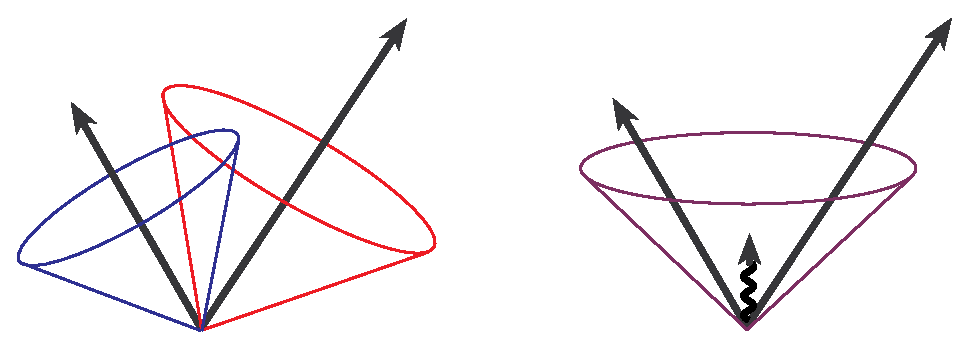
\includegraphics[width=0.8\textwidth]{Diagrams/cone-fig1.eps}
\caption[Infra-red sensitivity of a basic cone algorithm]{Infra-red sensitivity of a basic cone algorithm \cite{Blazey:2000qt}. The two hard partons, represented as arrows, are separated by more than $R_{cone}$ but less than $2R_{cone}$. In the absence of radiation between the jets (left), 2 distinct jets will be found. However, radiation between the jets (right) would cause only 1 jet to be found. \label{infraredcone}}
\end{figure}

This problem is removed if, in addition to using the particles as seeds, a seed is created in the middle (in $\eta \times \phi$) of every two particles that are separated by less than $2R_{cone}$. Now the final result is independent of soft radiation. This type of algorithm is called a mid-point cone algorithm.

\subsection{The $K_T$ Clustering Algorithm}

The $K_T$ algorithm is kinematically motivated. The prescription is to merge particles together if they have a low transverse momentum with respect to one another. The basic inclusive $K_T$ algorithm, outlined in \cite{Butterworth:2002xg}, defines jets in the following way:

\begin{enumerate}

\item The resolution variables, $d_{kB}$ and $d_{kl}$, are computed for every object, $k$, and every pair of objects, $k$ and $l$. The resolution variables are defined to be
\begin{equation*}
d_{kB} = p_{Tk}^2 \qquad \text{and}
\end{equation*}
\begin{equation}
d_{kl} = \text{min}\left(p_{Tk}^2, p_{Tl}^2\right)\left[\left(\eta_k - \eta_l\right)^2 + \left(\phi_k - \phi_l\right)^2\right]  \, .
\end{equation}
At the start of the algorithm, the list of objects are particles or calorimeter towers.

\item The $d_{kB}$ are scaled by 
\begin{equation}
d_k = R_{K_T}^2 d_{kB}
\end{equation}
where $R_{K_T}$ is a user defined parameter.

\item The smallest resolution variable is found in the set of $d_k$ and $d_{kl}$. If this is one of the  $d_{kl}$, then objects $k$ and $l$ are merged into a single object. If one of the $d_k$ is the smallest resolution variable then $k$ is defined as a jet and removed from the list.

\item Steps 1 - 3 are repeated until all objects are defined as jets.

\end{enumerate}
This algorithm is insensitive to soft or collinear radiation. It is the nature of the $K_T$ algorithm to merge soft/collinear particles first because these have the smallest $d_{kl}$ resolution variable. 




\section{Central Exclusive Jet Variables} \label{excvars}

Assuming the outgoing protons are tagged, there are a number of kinematic variables that can be measured in the central system and matched to the information from FP420. In this section, the variables of interest in a di-jet analysis are introduced. The fraction of proton momentum that enters the hard-subprocess can be estimated by
\begin{equation}
x_{1, 2} \simeq \frac{1}{\sqrt{s}} \sum_i E_{T}^i e^{\pm \eta_i}
\end{equation}
where the sum is over the highest two transverse energy jets \cite{Collins:1997nm, Affolder:2000hd} and $s$ is the collision centre-of-mass energy of the incoming beams. The values of $x_1$ and $x_2$ can be combined to obtain the di-jet mass $M_{jj}^2 \simeq x_1x_2s$. The variable $R_{jj}$, given by
\begin{equation}
R_{jj} = \frac{M_{jj}}{M},
\end{equation}
measures the fraction of the central system mass that is contained in the di-jets \cite{Affolder:2000hd}. The measurement of the mass, $M$, by FP420 is given by equation \ref{missingmass}. Therefore, the central exclusive condition , $x=\xi$, should result in $R_{jj}=1$. In practice, parton showering and jet finding inefficiencies result in the actual $R_{jj}$ being somewhat less than 1.0 and in the case of hard final state radiation, the value of $R_{jj}$ could be much lower than 1.0.

To combat the problem of hard final state radiation, a new measure of the di-jet mass fraction has been introduced \cite{Khoze:2006iw}. The new variable, $R_j$, is motivated by the knowledge that the highest transverse energy jet in the event will have been least affected by hard final state parton showering. $R_j$ is defined as 
\begin{equation}
R_j = \frac{2E_T}{M}\cosh\left(\eta_j - y \right)
\end{equation}
where $\eta_j$ and $E_T$ are the pseudorapidity and transverse energy  of the leading (highest transverse energy) jet and $y$ is the rapidity of the central system given by equation \ref{ceprapidity}.

A further consequence of tagging the outgoing protons is
that the rapidity of the central system can be measured by both FP420 and the central detector. The difference in these measurements, $\Delta y$, given by 
\begin{equation}\label{deltaydef}
\Delta y = y - \frac{\left(\eta_1 + \eta_2 \right)}{2}    ,
\end{equation}
should be approximately zero for the exclusive final state. Note the use of pseudo-rapidity for the jets in the central system. Pseudo-rapidity is a good approximation to rapidity if the transverse momentum of the jet satisfies $p_T \gg m$, where $m$ is the mass of the parton in the hard scatter that produces the jet.
%where the approximation $y\rightarrow\eta$ has been used assuming $p_T \gg m_b$. 
The first term on the right hand side of equation \ref{deltaydef} is the rapidity of the central system measured by FP420, whilst the second term is simply the average pseudo-rapidity of the highest two transverse energy jets.

Finally, it is possible to examine the activity outside of the di-jet system. In central exclusive and double pomeron exchange events, the protons are not colour connected to the central system. This results in rapidity gaps between the outgoing protons and the central system. In the absence of pile-up, the rapidity gaps can be used to identify these events by requiring low activity in the calorimeters in the high rapidity regions. However, at nominal low luminosity running at the LHC, there are on average 3.5 interactions per bunch crossing, which can destroy the rapidity gap.

This does not mean that one cannot look at activity outside of the di-jet system. The excellent vertex resolution of the ATLAS detector allows charged tracks to be associated with specific vertices, even in the presence of pile-up. Because the protons remain intact, there are no multiple interactions and one would expect few extra tracks, $N_C$, associated with the di-jet vertex but outside of the di-jet system. The exact cut off will be jet parameter dependent. 
A better measure of the activity outside of the di-jets could be the number of charged tracks, $N_{C}^{\perp}$, that are transverse to the leading jet. $N_{C}^{\perp}$ is defined as the number of charged tracks in the ranges 
\begin{equation} \label{ncperp}
\frac{\pi}{3}<|\phi_{k} -\phi_j|<\frac{2\pi}{3} \quad \text{and} \quad \frac{4\pi}{3}<|\phi_{k} -\phi_j|<\frac{5\pi}{3}  
\end{equation}
where $j$ labels the leading jet and $k$ a charged track associated with the di-jet vertex.
%%ncharged
%%ncharged CDF
\section{Central Exclusive $H \rightarrow b\bar{b}$ at ATLAS} 

The aim of this section is to determine whether it is possible to observe the $b\bar{b}$ decay channel of a Higgs boson in central exclusive production at ATLAS. It has already been shown that the $WW^{*}$ decay channel is adequate for discovering the Standard Model Higgs using FP420 for 140~$\leq m_H \leq$~200~GeV \cite{Cox:2005if}. Therefore, in this analysis, the choice of Higgs mass is $m_H = 120$ GeV.

The choice of jet algorithm will affect the reconstructed exclusive variables and hence the choice of cut required to remove the background. The strategy here is to firstly extract the best kinematic matching cuts between the central system and FP420 for each jet algorithm. Further possible exclusivity requirements are then examined in order to reduce the non-exclusive backgrounds. Finally, the cross sections and significance of discovery are presented, along with the impact of possible experimental triggers.

\subsection{Backgrounds}

The backgrounds to the central exclusive $H \rightarrow b\bar{b}$ channel are divided into three categories; central exclusive, double pomeron exchange and overlap. The central exclusive backgrounds are $gg\rightarrow b\bar{b}$ and $gg\rightarrow gg$ and are simulated, along with the Standard Model Higgs signal, using the ExHuME Monte Carlo. The $b\bar{b}$ and $gg$ backgrounds are generated in the mass range $80 \leq M \leq 160$~GeV with a $|\cos\theta| \leq 0.98$ cut in the CM frame. 

%However, equation \ref{exclusivediquark} shows that the exclusive di-quark background is, at a given central mass, strongly peaked in the large pseudo-rapidity region. Hence an $E_T$ and $\eta$ cut will reduce this background. The $gg$ background can be reduced in a similar way. 

The double pomeron exchange processes are simulated using the POMWIG event generator \cite{Cox:2000jt}. As FP420 has acceptance for small values of $\xi$, the processes are generated using the \Pom \Pom \, fusion process without the contribution from the subleading reggeon, which is expected to be small.  POMWIG is normalised to H1 data \cite{Adloff:1997sc} and does not contain a value of the soft survival factor. For the purposes of this analysis, the soft-survival is set to 0.03 \cite{Alekhin:2005dx:Soft}. There are two DPE processes that act as background: $b\bar{b}$ and $jj$, where the $j$ are light quark and gluon jets. These backgrounds have two intact protons in the final state and a jet-like central system. However, the kinematics of the two-jet event measured in the ATLAS detector should not match the kinematics measured in FP420 because of the presence of pomeron remnants in the final state. Section \ref{kinematicmatch} deals with the correct identification of these events.

The overlap background involves two single diffractive (SD) events, which produce the protons measured in FP420, plus a QCD di-jet event all in one bunch crossing at the LHC. The relevant QCD processes are again $b\bar{b}$ and $jj$ and are generated using the HERWIG event generator. However, the protons from the SD events have absolutely no relation to the QCD event and as such, one would expect the kinematics to very rarely match between FP420 and the central ATLAS detector. Furthermore, the protons that gave rise to the QCD event have broken up, which deposits extra energy in the calorimeters and leaves extra tracks in the inner detector. This type of background is covered in more detail in section \ref{overlap}.

\subsection{Jet Algorithm effects and Kinematic Matching Cuts}\label{kinematicmatch}

Starting with just the $H\rightarrow b\bar{b}$ signal events, the two types of jet algorithm were applied. Events  were only retained if the highest transverse energy jet had $E_T > 40$~GeV. This choice is motivated by the transverse energy of the $b$-quarks peaking at 60~GeV if $m_H=120$~GeV (figure \ref{bquarket}) in addition to the  steep transverse energy dependence of the central exclusive backgrounds (figure \ref{dipartonplots} (a)). The effects of the cone and inclusive $K_T$ algorithms on the reconstructed $R_{jj}$
distribution are shown in figure \ref{higgsrjj}.
The $R_{jj}$ distribution has a peak close to 1.0 but a long tail to medium $R_{jj}$ values. This is due to hard final state radiation from one of the $b$ quarks not being recovered by the jet algorithm. The effect of reducing the cone radius results in less of the energy being reconstructed in the two-jet system and a flatter $R_{jj}$ distribution as expected. Reducing $R_{K_T}$ has a similar effect.


\begin{figure} 
\centering
\mbox{
	\subfigure[]{\epsfig{figure=Diagrams/HiggsRJJDiffCone.eps,width=0.5\textwidth,height = 6cm}}
	\subfigure[]{\epsfig{figure=Diagrams/HiggsRJJDiffKTR.eps,width=0.5\textwidth,height = 6cm}}
}
\caption[The effect of the cone and $K_T$ algorithms on the signal $R_{jj}$ distribution]{The reconstructed signal $R_{jj}$ distribution using the cone (a) and $K_T$ (b) jet-finding algorithms. The effect of changing $R_{cone}$ or $R_{K_T}$ is also shown. \label{higgsrjj}}
\end{figure}

In contrast, the variable $R_j$ is defined to be less affected by very hard radiation from one of the jets.
The $R_j$ distribution, shown in figure \ref{higgsrj}, has a narrower peak than the $R_{jj}$ distribution with the long tail removed. Furthermore, changing the jet algorithm parameter has less effect on the distribution -  decreasing $R_{cone}$ or $R_{K_T}$ results in only a small shift to lower values of $R_j$ as progressively more soft particles are not reconstructed in the highest transverse energy jet. This makes $R_j$ a robust variable for defining exclusive events. The $K_T$ algorithm performs slightly better than the cone algorithm because the distribution is less susceptible to changes in $R_{K_T}$. Both algorithms produce similar shapes of distribution.


\begin{figure} 
\centering
\mbox{
	\subfigure[]{\epsfig{figure=Diagrams/HiggsRJDiffCone.eps,width=0.5\textwidth,height = 6cm}}\quad
	\subfigure[]{\epsfig{figure=Diagrams/HiggsRJDiffKTR.eps,width=0.5\textwidth,height = 6cm}}
	%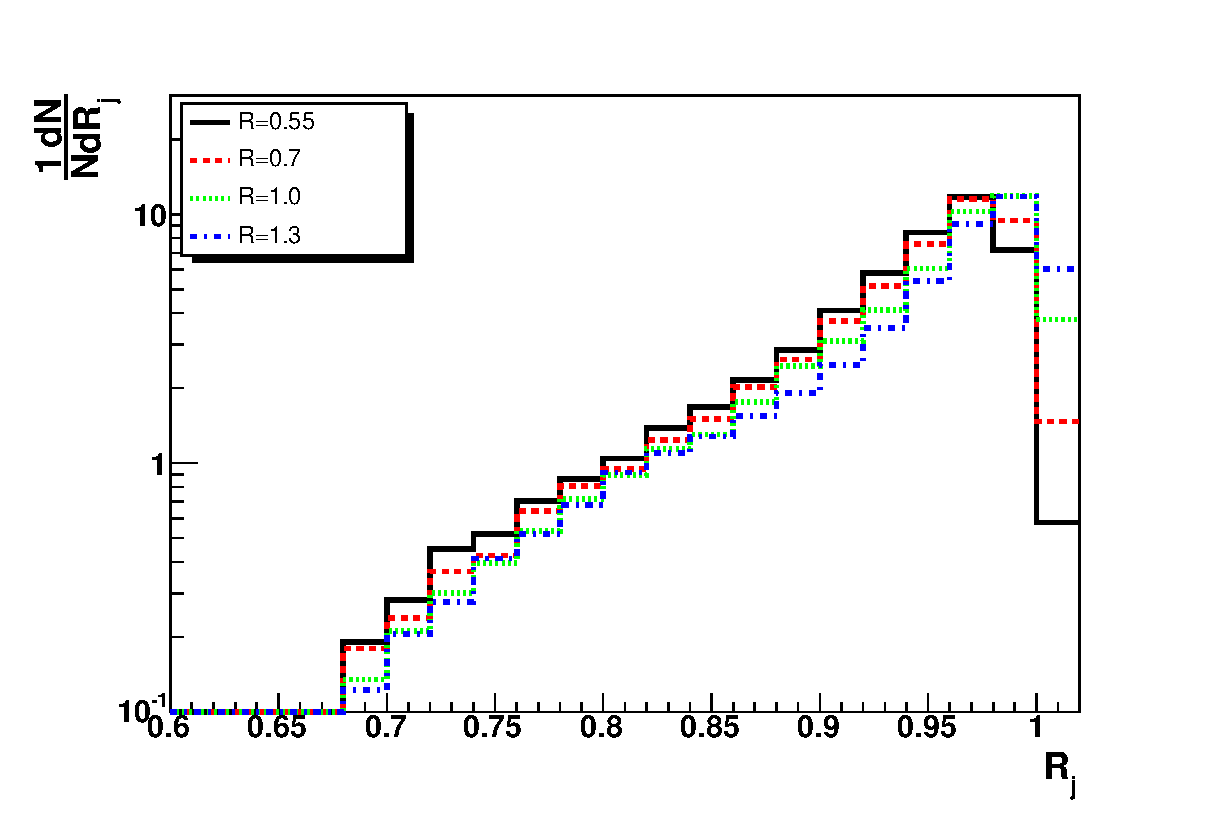
\includegraphics[width=0.5\textwidth]{Diagrams/HiggsRJDiffKTR.eps}
	}
\caption[The effect of the cone and $K_T$ algorithms on the signal $R_{j}$ distribution]{The reconstructed signal $R_{j}$ distribution using the cone (a) and $K_T$ (b) jet-finding algorithms. The $R_j$ distribution less sensitive to changes in $R_{cone}$ or $R_{K_T}$ than $R_{jj}$. \label{higgsrj}}
\end{figure}


The final kinematic matching variable, $\Delta y$, is shown in figure \ref{higgsdeltay}.  Both distributions have the majority of events concentrated in the region $\Delta y < 0.1$. The conclusion is that the $R_j$ and $\Delta y$ variables are extremely good at defining the exclusive event. Furthermore, it is possible to choose small values of $R_{cone}$ or $R_{K_T}$ without too much change in the reconstructed signal. This will be important in high luminosity running at the LHC, where 35 events are expected in every bunch crossing. Smaller values of $R_{cone}$ and $R_{K_T}$ will result in less particles from the pile-up being wrongly added into the jets of interest.

\begin{figure} 
\centering
	\mbox{
	\subfigure[]{\epsfig{figure=Diagrams/HiggsDeltaEtaDiffCone.eps,width=0.5\textwidth,height = 6cm}}
	\subfigure[]{\epsfig{figure=Diagrams/HiggsDeltaEtaDiffKTR.eps,width=0.5\textwidth,height = 6cm}}
	}
\caption[The effect of the cone and $K_T$ algorithms on the signal $\Delta y$ distribution]{The reconstructed signal $\Delta y$ distribution using the cone (a) and inclusive $K_T$ (b) jet-finding algorithms.\label{higgsdeltay}}
\end{figure}

The objective now is to define a set of exclusivity cuts that keep as much of the signal as possible, whilst rejecting a large fraction of the background. The $R_{jj}$, $R_j$ and $\Delta y$ distributions for the central exclusive Higgs are plotted in figure \ref{fig:higgsvsdpebb} against the $b\bar{b}$ background produced via double pomeron exchange. A cone radius of 0.4 and a $K_T$ R-parameter of 0.55 are used, and the distributions are normalised to the same area. It should be noted that, at this stage, the double pomeron exchange $b\bar{b}$ cross section is approximately 380 times larger than the signal although spread over a larger mass range. 

\begin{figure} 
\centering
\mbox{
	\subfigure[]{\epsfig{figure=Diagrams/HiggsvsDPEbb_RJJcone0.4.eps,width=0.5\textwidth,height = 6cm}}\quad
	\subfigure[]{\epsfig{figure=Diagrams/HiggsvsDPEbb_RJJkti0.55.eps,width=0.5\textwidth,height = 6cm}} 
	}
\mbox{
	\subfigure[]{\epsfig{figure=Diagrams/HiggsvsDPEbb_RJcone0.4.eps,width=0.5\textwidth,height = 6cm}}\quad
	\subfigure[]{\epsfig{figure=Diagrams/HiggsvsDPEbb_RJkti0.55.eps,width=0.5\textwidth,height = 6cm}}
	}
\mbox{
	\subfigure[]{\epsfig{figure=Diagrams/HiggsvsDPEbb_DeltaEtacone0.4.eps,width=0.5\textwidth,height = 6cm}}\quad
	\subfigure[]{\epsfig{figure=Diagrams/HiggsvsDPEbb_DeltaEtakti0.55.eps,width=0.5\textwidth,height = 6cm}}
}
\caption[Comparison of the $R_{jj}$, $R_j$ and $\Delta y$ distributions for exclusive Higgs and double pomeron $b\bar{b}$ events ]{The normalised $R_{jj}$, $R_j$ and $\Delta y$ distributions for exclusive Higgs and double pomeron $b\bar{b}$ production, using a cone radius of 0.4 (a, c, e) and inclusive $K_T$ R-parameter of 0.55 (b, d, e).\label{fig:higgsvsdpebb}}
\end{figure}

The values $R_{cone}=0.4$ and $R_{K_T} = 0.55$ are chosen for two reasons. Firstly, they produce similar distributions and do not give a false impression that one algorithm is superior. Secondly, these smaller values of $R_{cone}$ and $R_{K_T}$ are less likely to reconstruct di-jets containing some of the pomeron remnants. This is desirable in order to reconstruct the hard-scattering part of the double pomeron exchange process. The difference between DPE and CEP events is obvious and expected, the presence of pomeron remnants means that the kinematics of the hard sub-process does not match the kinematics measured in FP420.

Using $R_j$ instead of $R_{jj}$ has some interesting effects. Firstly, as expected, the low $R_{jj}$ tail is not present in the $R_j$ distribution for both the signal and background. This initially leads to the presumption that the $R_j$ variable is better at reconstructing the mass of the hard-scatter than $R_{jj}$. However, for the double pomeron $b\bar{b}$ events, the $R_j$ distribution extends to higher values than $R_{jj}$. Some of this increase can be attributed to the highest transverse energy jet containing some pomeron remnant. This extra energy is then counted twice in the $R_j$ reconstruction. This problem is reduced by the use of small values of $R_{cone}$ and $R_{K_T}$ but can never be completely removed.
The second effect of using the $R_j$ variable is that there is a sharper, more distinct separation between the signal and background when compared to the $R_{jj}$ variable. This is mainly due to the long tail in the signal $R_{jj}$ distribution. 

%The $\Delta y$ distribution is also well reconstructed. Smaller values of $R_{cone}$ or $R_{K_T}$ lead to a broader distribution with a long tail to large values of $\Delta y$. This is because hard radiation in the parton showering phase would lead to a significant change in direction of one of the jets if the energy from the radiation is reconstructed as a third jet.

The distributions presented in figure \ref{fig:higgsvsdpebb} give a feel for the loosest possible cuts in those distributions. The loose cut is defined as the point at which the normalised signal and background distributions cross over. For example, a cut of $R_j >$ 0.85 can be applied to di-jets reconstructed using the inclusive $K_T$ algorithm with $R_{K_T}=0.55$. Moving this cut to lower $R_j$ would include a larger fraction of background with only a very small gain in signal. This loose cross-over cut is not the optimum cut for the analysis because the unnormalised background is so much larger than the signal; it only indicates the region of interest for further study. The best cut is determined later by requiring a favourable ratio of signal to all background.
%\afterpage{
%\clearpage

\begin{figure}
\centering
\mbox{ 
	\subfigure[]{\epsfig{figure=Diagrams/ConeDijetMassFractionCut.eps,width =.5\textwidth}}
	\subfigure[]{\epsfig{figure=Diagrams/KTDijetMassFractionCut.eps,width=.5\textwidth}}
	}
\caption[The dependence of the $R_{jj}$ and $R_{j}$ cuts on $R_{cone}$ and $R_{K_T}$]{The dependence of the $R_{jj}$ and $R_{j}$ cuts as a function of $R_{cone}$ (a) and $R_{K_T}$ (b).\label{dijetmasscutsvsparam}}
\end{figure}
%}

The cut value depends on the values of $R_{cone}$ or $R_{K_T}$ used to reconstruct the di-jets. Figure \ref{dijetmasscutsvsparam} shows how the cross-over cut values for $R_{jj}$ and $R_{j}$ change with the jet algorithm parameter. 
Using the $K_T$ algorithm as an instructive example, it is clear that the $R_j$ cut is less dependent on $R_{K_T}$ than the $R_{jj}$ cut. The steep dependence of the $R_{jj}$ cut with $R_{K_T}$ is easily understood, because the signal is reconstructed with larger $R_{jj}$ when $R_{K_T}$ is increased (figure \ref{higgsrjj} (b)). 
Furthermore, the background will also be reconstructed with larger $R_{jj}$ as it is just as susceptible to parton showering. Therefore the cut naturally increases to keep the signal efficiency high and the background efficiency low. A similar effect is found for the cone algorithm, but the dependence is less steep with $R_{cone}$

The $R_j$ cut however, has a weaker dependence on the value of $R_{K_T}$ used to define the jets. Figure \ref{higgsrj} showed that the reconstructed signal shape is almost $R_{K_T}$ independent. The only change is a small shift to larger $R_{j}$ as the value of $R_{K_T}$ is increased. It is natural to assume that the background would follow the same trend. These larger values of $R_{K_T}$ are more likely to pull in some of the remnants, thus the cut increases to keep the background efficiency low. The performance of the cone algorithm is similar across the range of $R_{cone}$ used. 

The $\Delta y$ cut is always less than 0.1 and decreases with $R_{K_T}$ because there is less chance of parton showering changing the direction of a jet.  The cut on $\Delta y$ is not examined further because it is smaller than the granularity of the towers in the hadronic calorimeter. It is not obvious that the direction of a jet can be measured more accurately than the tower granularity and so the exclusivity cut is set at $\Delta y < 0.1$ for the rest of the analysis.

The reconstructed signal and background efficiencies as a function of $R_{cone}$ and $R_{K_T}$ are shown in figure \ref{dijetmasscutefficiency}. For each jet algorithm parameter, the preferred cuts given in figure \ref{dijetmasscutsvsparam} are used. 
For the signal, the performance of the cone and $K_T$ algorithms are similar. In the case of the $R_j$ cut, the efficiency is approximately flat with a slight decrease at large and small values of $R_{cone}$ and $R_{K_T}$. In contrast, the efficiency of the $R_{jj}$ cut increases with both $R_{cone}$ and $R_{K_T}$. This is a direct consequence of the flatter $R_{jj}$ distributions at smaller $R_{cone}$ and $R_{K_T}$, which result in less signal events in the region of interest. In all cases, the best efficiency for signal reconstruction occurs after cuts on the $R_j$ variable. 

%For the signal, the performance of the cone and $K_T$ algorithms are very similar. For $R_j$, the signal efficiency is virtually independent of both $R_{cone}$ and $R_{K_T}$ being flat at about $87\%$. For $R_{jj}$, the efficiency of the signal increases with $R_{cone}$ and $R_{K_T}$. In all cases, the signal efficiency is always better for loose cuts on $R_{j}$ than $R_{jj}$. 

The reconstructed double pomeron background is more interesting. The percentage of events passing the $R_{jj}$ cut decreases as $R_{cone}$ or $R_{K_T}$ increases. This contradicts the expectation that increasing the jet algorithm parameter would result in more of the pomeron remnants being reconstructed in the di-jets for DPE processes.
However, as previously stated, the $R_{jj}$ cut increases with $R_{cone}$ or $R_{K_T}$ because more signal events are reconstructed at high $R_{jj}$. The only explanation is that the improved signal reconstruction cancels the effect of more pomeron remnants being added into the jets. A similar result is found for the cone algorithm when applying an $R_{j}$ cut.

The $K_{T}$ algorithm on the other hand shows completely different dependence for the $R_j$ variable. The percentage of background events passing the $R_j$ cut initially decreases with $R_{K_T}$ if a cut on $R_{j}$ is made. However, at larger values of $R_{K_T}$ the percentage of events passing the cut begins to increase again. The explanation is that, at these larger values of $R_{K_T}$, the probability of pomeron remnants being reconstructed in the highest $E_T$ jet increases, while the signal distribution remains relatively unaffected. The cone algorithm does not show this because the signal $R_j$ distribution changes more with $R_{cone}$ than with $R_{K_T}$ (figure \ref{higgsrj}). 

\begin{figure} 
\centering
\mbox{
	\subfigure[]{\epsfig{figure=Diagrams/ConeDijetMassFractionSignalEfficiency.eps,width =.5\textwidth}}\quad
	\subfigure[]{\epsfig{figure=Diagrams/ConeDijetMassFractionBackgroundEfficiency.eps,width =.5\textwidth}}
	}
	\mbox{
	\subfigure[]{\epsfig{figure=Diagrams/KTDijetMassFractionSignalEfficiency.eps,width =.5\textwidth}}\quad
	\subfigure[]{\epsfig{figure=Diagrams/KTDijetMassFractionBackgroundEfficiency.eps,width =.5\textwidth}}
}
\caption[The efficiency of the $R_{jj}$ and $R_{j}$ cuts as a function of $R_{cone}$ and $R_{K_T}$]{The efficiency of the $R_{jj}$ and $R_{j}$ cuts as a function of $R_{cone}$ and $R_{K_T}$ for the central exclusive Higgs (a,c) and DPE $b\bar{b}$ (b,d) processes.\label{dijetmasscutefficiency}}
\end{figure}

With the small cross sections involved in central exclusive production, it is important to retain as much signal as possible. Furthermore, the cuts should be chosen to minimise the effect of experimental conditions at the LHC. The first point of note is that large values of $R_{K_T}$ and $R_{cone}$ will be more affected by pile-up than smaller values, which implies that smaller values of $R_{cone}$ and $R_{K_T}$ are desirable. With this in mind it is sensible to cut on the $R_j$ variable as the signal efficiency is independent of $R_{cone}$ and $R_{K_T}$. In the case of the $K_T$ algorithm, the natural choice is then to use $R_{K_T} = 0.55$ because this results in the lowest percentage of background events passing the cut (figure \ref{dijetmasscutefficiency} (d)).
 For the cone algorithm, the choice is less straightforward. The plots presented in figure \ref{dijetmasscutefficiency} would indicate that large values of $R_{cone}$ should be used in order to reduce the background by a large value. However, the pile-up issues require small values of $R_{cone}$. As a compromise, the intermediate value of $R_{cone} = 0.4$ is chosen.

The finalised kinematic matching cuts are determined by the jet algorithm parameter and are presented in table \ref{kinematch}. The upper window on $R_{j}$ is chosen after consideration of detector resolution. In \cite{:1999fq:Chapter9}, the offline reconstructed jet resolution was found to be $8.5\%$ for jets with an energy of 50~GeV, which is the approximate energy of the jets in this analysis. The resolution of the $R_j$ variable is dominated by this energy resolution because the FP420 mass resolution is expected to be approximately 2\%. This means that the $R_j$ variable should not be constrained by a window smaller than $0.9<R_j<1.1$, which leaves open the possibility of tightening the lower bounds in $R_{j}$ later if necessary.

\begin{table}[t]
\centering
\begin{tabular}{|c|c|c|}
\hline
Cut & $R_{K_T}=0.55$ & $R_{cone}=0.4$ \\
\hline
$R_{j}^{min}$ & 0.85 & 0.82 \\
$R_{j}^{max}$ & 1.10 & 1.10 \\
$\Delta y$ & 0.1 & 0.1 \\ 
\hline
\end{tabular}
\caption[Kinematic matching cuts to distinguish between the DPE and CEP processes]{The finalised kinematic matching cuts for the cone and $K_T$ algorithms. The $R_j^{min}$ cut was chosen to be the point at which the normalised double pomeron exchange $b\bar{b}$ and central exclusive $H\rightarrow b\bar{b}$ distributions crossed over. The $R_{j}^{max}$ and $\Delta y$ cuts were chosen after consideration of detector effects. \label{kinematch}}
\end{table}%


\subsection{Simulation of the Overlap Background}\label{overlap}

The overlap background is defined as a threefold coincidence of a QCD event and two single diffractive events all in one bunch crossing at the LHC. The overlap background cross section, $\sigma_{\text{olap}}$, can be estimated by 
\begin{equation}\label{overlapxs}
\sigma_{\text{olap}} = \left(N-1\right)\left( N-2\right) \,  P_1 \,  P_2 \, ~Q ~\sigma
\end{equation}
where $N$ is the number of interactions per bunch crossing, $Q$ is the QUARTIC rejection factor and the $P_i$ are the probabilities of an event at the LHC being a single diffractive event that causes a proton hit in FP420.  The labels 1 and 2 indicate the beam to which the single diffractive proton belongs. The input cross section, $\sigma$, is the cross section of the normal inclusive QCD events.

The number of interactions per bunch crossing at the LHC is luminosity dependent and is given in equation \ref{LHCoverlap}. QUARTIC performs the measurement of the time-of-flight difference of the two scattered protons. 
As stated in section \ref{fp420}, this gives a measurement of the interaction vertex to an accuracy of 2.1~mm. In the case of the overlap backgrounds, a fake vertex is reconstructed from the two single diffractive protons. This vertex does not, in general, coincide with the QCD event vertex.

The QUARTIC rejection factor is calculated by picking three random points according to a gaussian distribution of width 5.6~cm, which is the longitudinal beam spot size at the LHC \cite{:1999fq:Chapter3}. Two of these points correspond to the SD vertices and the average corresponds to the fake vertex measured by QUARTIC. If the final point, which corresponds to the primary QCD vertex, is within 2.1~mm of the fake vertex, then the event will pass the QUARTIC measurement. It is found that only 2.5\% of overlap events satisfy this requirement. 
%This is in good agreement with \cite{brandt}.

The $P_i$ are found using the single diffractive cross section, $\sigma_{SD}$, which is given \cite{Khoze:2006gg} by
\begin{equation} \label{sdxs}
\frac{1}{\sigma_T}\frac{d\sigma^{SD}}{dtdx_L} = \frac{g_N^2(t) g_{3\text{\Pom}}}{16\pi^2 g_N(0)}
\left(1 - x_L \right)^{\alpha_{\text{\Pom}}(0) - 2 \alpha_{\text{\Pom}}(t)} S_{SD}^2(s,t)
\end{equation}
where $\sigma_{T}$ is the total cross section, $x_L=1-\xi$ and $g_{3\text{\Pom}}(t) = g_N(0)/3$ is the triple pomeron vertex. 
The soft-survival factor for single diffraction, $S_{SD}^2$, is taken to be 0.085 at the LHC \cite{Khoze:2006gg}. 
The pomeron-nucleon coupling, $g_N(t)$, is given by 
\begin{equation}
g_N(t) = 8 \, \left( \frac{3.52 - 2.79t}{3.52 -t} \right) \frac{1}{\left(1 - \frac{t}{0.71}\right)^2}
\end{equation}
and the Regge trajectory of the pomeron, $\alpha_{\text{\Pom}}(t)$, by\footnote{The actual pomeron trajectory used in \cite{Khoze:2006gg} differs from the standard soft pomeron trajectory of Donnachie and Landshoff \cite{Donnachie:1992ny}. This is necessary in the new approach to both fit the data and account for rescattering corrections. The triple pomeron vertex is also different for similar reasons. The author would like to thank Misha Ryskin for clarification on this issue.}
\begin{equation}
\alpha_{\text{\Pom}}(t) = 1.11 + 0.07t.
\end{equation}
Each $P_i$ is calculated by integrating equation \ref{sdxs} over the FP420 acceptance range for $\xi$ given in section \ref{fp420}. This results is $P_1 = 0.85\%$ and $P_2=0.86\%$. 

The overlap cross section can then be reduced by kinematic matching. The overlap background events are constructed in two steps. The proton $\xi_{1,2}$ and $t_{1,2}$ values are constructed using equation \ref{sdxs} and the Monte Carlo methods presented in section \ref{mcdist}. The values of $t$ are distributed in the range $\{-3,0\}$ and the values of $\xi$ in the FP420 acceptance range.
The QCD event is generated using HERWIG, with JIMMY used for the underlying event  \cite{Butterworth:1996zw}. JIMMY calculates the number of secondary scatters during a proton-proton collision and has two main input parameters: PTJIM specifies the minimum transverse momentum of a secondary scatter and JMRAD(73) specifies the inverse square proton radius. JIMMY has been tuned to Tevatron data \cite{Alekhin:2005dx:MPITune} with PTJIM$=$3~GeV and JMRAD(73)$=$2.13. 

\subsection{Further Exclusivity Requirements}\label{exclusivityreq}

It is now possible to estimate the signal-to-background ratio for central exclusive $H\rightarrow b\bar{b}$ using the following cuts on the MC samples:
\begin{enumerate}
\item The $K_T$ and cone algorithms are used, with $R_{K_T} = 0.55$ or $R_{cone}=0.4$.
\item The highest transverse energy jet must satisfy $E_T > 40$~GeV.  
\item The longitudinal momentum loss of the protons must lie in the FP420 acceptance range,  $0.0023<\xi_1<0.0129$ and $0.0029<\xi_2<0.0171$.
\item The di-jet mass fraction must be in the range $0.85 < R_j <1.10$ for the $K_T$ algorithm or $0.82< R_j <1.10$ for the cone algorithm.
\item The difference between the rapidity of the central system measured by FP420 and the average jet pseudo-rapidity should satisfy $\Delta y < 0.1$.
\end{enumerate}
The first requirement is the choice of jet finding parameter discussed in section \ref{kinematicmatch}. The second cut is motivated by the transverse energy distributions of the Higgs decay products peaking at $\frac{m_H}{2}$. The third cut limits the protons to produce a hit in FP420. The final two cuts reduce the  background by kinematic matching as discussed in section \ref{kinematicmatch}. The subsequent analysis is carried out with both the cone and $K_T$ algorithms, but all the plots presented in this section are for the $K_T$ algorithm unless explicitly stated. The final results are presented for both cone and $K_T$ algorithms.

\begin{figure}
\centering
%\mbox{ 
	\subfigure[]{\epsfig{figure=Diagrams/DeltaRb.eps,width =.5\textwidth}}
%	\subfigure[]{\epsfig{figure=Diagrams/KTDijetMassFractionCut.eps,width=.5\textwidth}}
%	}
\caption[The distance, in $\eta$-$\phi$ space, between the jets and a $b$ quark for a HERWIG $+$ JIMMY $b\bar{b}$ sample]{The distance, in $\eta$-$\phi$ space, of jets with transverse energy greater than 10~GeV from a $b$ quark in the HERWIG $+$ JIMMY $b\bar{b}$ sample.\label{bquarkjets}}
\end{figure}

Potential signal events are those in which the highest two transverse energy jets are tagged as $b$-jets. Because of this, a rudimentary $b$-tagging procedure is applied to the MC samples. For the $b\bar{b}$ samples, a jet is defined to originate from a $b$-quark if the distance
\begin{equation}
\Delta R_{b} = \sqrt{\left(\phi_{j}-\phi_b\right)^2 + \left(\eta_{j}-\eta_b\right)^2}
\end{equation}
between the jet, $j$, and the $b$-quark, $b$, is smaller than a specified amount. Figure \ref{bquarkjets} shows the $\Delta R_{b}$ distribution for the HERWIG $b\bar{b}$ sample using all jets with transverse energy greater than 10~GeV. There is a clear minimum in the distribution and a $b$-jet is therefore defined by $\Delta R_{b} \leq 0.4$. The jets in the $gg$ and light quark samples are assumed to be non $b$-jets.

This designation of jets is necessary because the $b\bar{b}$ final state in the HERWIG samples is often constructed by $gb$ scattering, with the $\bar{b}$ quark produced in the intial state parton shower. In this case, the highest two transverse energy jets will not both originate from $b$ quarks and have a lower probability of being tagged as a $b\bar{b}$ event.
The experimental $b$-tagging efficiency at ATLAS, which is assumed to be 0.6 for a $b$-jet and 0.013 for light quark and gluon jets \cite{:1999fq}, is applied to the two highest transverse energy jets. Thus, each event in the samples is assigned a probability to be tagged as $b\bar{b}$; the tagging probability is 0.36 if the two highest transverse energy jets are both $b$-jets, 0.0078 for $gb$ and $g\bar{b}$ systems and 1.69$\times10^{-4}$ for $gg$ and $jj$.

\begin{table}[tdp]
\centering
\begin{tabular}{|c|c|r|r|}
\hline
Generator & Process & \multicolumn{2}{c|}{Cross section (fb)} \\
& & $R_{K_T}=0.55$ & $R_{cone}=0.4$ \\
\hline
ExHuME & $H\rightarrow b\bar{b}$ & 0.083 & 0.078 \\
 &$b\bar{b}$ & 2.39 & 1.73 \\
 & $gg$ & 3.58 & 1.93\\
POMWIG & $b\bar{b}$ & 3.94 & 2.61\\
& $jj$ & 0.078 & 0.034\\
HERWIG + 2$\times$SD & $b\bar{b}$ & 69.2 & 44.9\\
& $jj$ & 4.52 & 2.57 \\   
\hline
\end{tabular}
\caption[Cross sections of $H\rightarrow b\bar{b}$ and backgrounds after kinematic matching cuts]{The cross sections for signal and background. All samples have had a $E_T > 40$ GeV cut applied to the leading jet and the $b$-tagging procedure applied to the two highest $E_T$ jets. The proton momentum losses were restricted to the FP420 acceptance range  $0.0023<\xi_1<0.0129$ and $0.0029<\xi_2<0.0171$. The cut $0.85<R_j<1.1$ has been applied when using the $K_T$ algorithm. The corresponding cut for the cone algorithm is $0.82<R_j<1.1$, and $\Delta y<0.1$ is applied for both algorithms. The overlap background is defined at a luminosity of $2\times10^{33}$~cm$^{-2}$~s$^{-1}$.\label{inputxs}}
\end{table}%

The cross sections, defined by the cuts at the beginning of this section and scaled by the $b$-tagging procedure, are shown in table \ref{inputxs}. The large $gg$ and $jj$ backgrounds have been significantly reduced by the $b$-tagging. 
The $H\rightarrow b\bar{b}$ cross section is just 0.08~fb and all subsequent cuts are chosen to limit the reduction in the signal. As the overlap background is luminosity dependent, it is quoted at a specific luminosity (2$\times10^{33}$~cm$^{-2}$~s$^{-1}$).

\begin{figure}
\centering
\mbox{
	%\subfigure[]{
	\epsfig{figure=Diagrams/All_Masskti0.55.eps,width =0.75\textwidth}%}
	%\subfigure[]{\epsfig{figure=Diagrams/All_RJAfterCutskti0.55.eps, width =.5\textwidth}}
	}
\caption[The simulated mass distributions of signal and background processes as measured by FP420]{The mass distributions of signal and background processes as measured by FP420. The mass, $M$, has been smeared by a gaussian of width 0.02$M$ to approximate the resolution of FP420. 
\label{massafterkinematics}}
\end{figure}

The backgrounds can be reduced by cutting a mass window around the Higgs peak. The mass distributions for the signal and background are shown in figure \ref{massafterkinematics} after smearing the central mass by a gaussian with a width of 2\%, which simulates the FP420 mass resolution. The background distributions are continuous across the region of interest, thus a mass window of 116~$\leq M \leq$124~GeV is applied to the samples. It is clear that after such a cut, the dominant background comes from the $b\bar{b}$ overlap events. Furthermore, 
%the DPE $b\bar{b}$, the exclusive $b\bar{b}$ and the exclusive $gg$ backgrounds remain larger than the signal. The $jj$ overlap background is approximately the same size as the signal and remains significant.
all of the backgrounds, with the exception of the DPE $jj$ process, remain larger than the signal.

%The $R_j$ distribution, after the cut on the mass measured in the pots, is shown in figure \ref{massafterkinematics}. It is clear that the $R_j$ window will have to be tightened to remove more background.



The overlap background can be reduced further by examining the number of charged tracks associated with the  di-jet vertex. As stated in section \ref{excvars}, an exclusive event only has tracks originating from the hard scatter associated with the primary jet vertex. The overlap events, however, have an inclusive QCD event as the primary vertex. This means that there will be extra particles from the secondary scatters and the break up of the protons. If these particles are charged and lie within the pseudo-rapidity coverage of the inner detector, it will be possible to make a cut on them. The underlying event measures introduced in section \ref{excvars}, $N_C$ and $N_C^{\perp}$, are calculated for charged tracks that have $p_T>0.5$~GeV and lie in the pseudo-rapidity range $|\eta| < 2.5$. The $N_C$ and $N_C^{\perp}$ distributions are shown in figure \ref{nchargedtracks} for the central exclusive Higgs, the DPE $b\bar{b}$ background and the $b\bar{b}$ overlap background. 

\begin{figure}
\centering
\mbox{
	\subfigure[]{\epsfig{figure=Diagrams/All_NChargedkti0.55.eps,width=0.5\textwidth,height = 6cm}}\quad
	\subfigure[]{\epsfig{figure=Diagrams/All_NChargedCDFkti0.55.eps,width=.5\textwidth,height = 6cm}}
	}
\caption[The number of charged tracks associated with the primary vertex]{The $N_C$ distribution (a). Charged particles are defined as tracks if they have $p_T\geq0.5$~GeV and $|\eta|\leq2.5$. Also shown (b) is the $N_C^{\perp}$ distribution which defines tracks that are perpendicular to jets (equation \ref{ncperp}).\label{nchargedtracks}}
\end{figure}

Clearly, the number of charged tracks associated with the primary vertex is a good discriminator for all diffractive events, not just exclusive ones, as shown in figure \ref{nchargedtracks}. 
%These cuts are chose to keep a large signal fraction. 
%It is concluded that the better discriminator is $N_C^{\perp}$ for two reasons. Firstly, the central exclusive distribution is narrower and more sharply peaked at zero. As the measure is intended to measure underlying event, $N_C^{\perp}$ gives a more intuitive result, i.e. that there is no underlying event in central exclusive events. Secondly, the $N_C$ distribution for the overlap background events remains much larger than zero for the majority of the events and the cut will remove the majority of this background.
The signal $N_C^{\perp}$ distribution is narrower than the $N_C$ distribution, which makes it a better measure of the underlying event activity. The $N_C$ distribution suffers because particles that are part of the hard scatter may not be reconstructed in the di-jets by the jet algorithm, hence the broader distribution. However, the $N_C$ distribution covers more of the $\phi$ space and therefore has more chance of picking up activity that is not part of the hard scatter. It is concluded that both cuts are required to remove the overlap background. The tight, underlying event cut, $N_C^{\perp}\leq1,$ is applied first to remove the majority of the background. The looser, $N_C\leq 5$ cut is then applied to the samples to remove events with a large number of particles outside of the transverse region but also outside of the jets.


\begin{figure}
\centering
\mbox{
	\subfigure[]{\epsfig{figure=Diagrams/NChargedBBQCD_pt.eps,width=0.5\textwidth,height = 6cm}}\quad
	\subfigure[]{\epsfig{figure=Diagrams/NChargedCDFBBQCD_pt.eps,width=.5\textwidth,height = 6cm}}
	}
\mbox{
	\subfigure[]{\epsfig{figure=Diagrams/NChargedBBQCD_eta.eps,width=0.5\textwidth,height = 6cm}}\quad
	\subfigure[]{\epsfig{figure=Diagrams/NChargedCDFBBQCD_eta.eps,width=.5\textwidth,height = 6cm}}
	}
	
\caption[The dependence of the $N_C$ and $N_C^{\perp}$ distributions on the minimum transverse momentum and pseudo-rapidity of the charged particles]{The effect on the $N_C$ distribution of $b\bar{b}$ overlap events of changing the minimum transverse momentum that a charged particle can have in order to produce hits in the inner detector (a). Also shown (b) is the effect on the $N_C^{\perp}$ distribution. Both distributions assume particles are detected in the full pseudo-rapidity range of the inner detector. Figures (c) and (d) show the effect on the $N_C$ and $N_C^{\perp}$ distributions of limiting the pseudo-rapidity range of charged particle tracks (with $p_T>0.5$~GeV). All plots are normalised to equal areas. \label{nchargeddependence}}
\end{figure}


The $N_C$ and $N_C^{\perp}$ cuts are dependent on the performance of the inner detector, specifically the lowest transverse momentum a particle can have and still be reconstructed as a track. The effect of changing the minimum transverse momentum on the $N_C$ and $N_C^{\perp}$ distributions is shown in figure \ref{nchargeddependence} (a) and (b). It is important that the inner detector be able to pick up particles with $p_T\simeq0.5$~GeV, otherwise the overlap background could increase by an order of magnitude. Figures \ref{nchargeddependence} (c) and (d) show the effect on the $N_C$ and $N_C^{\perp}$ distributions if the pseudo-rapidity range of the charged tracks is restricted. It is found that limiting the $\eta$ range does not affect the distributions as much as the minimum transverse momentum cut. %This observation is crucial later in the analysis.

\begin{figure}
\centering
\mbox{
	\subfigure[]{\epsfig{figure=Diagrams/All_JetEtakti0.55.eps,width=0.5\textwidth,height = 6cm}}\quad
	\subfigure[]{\epsfig{figure=Diagrams/All_JetPhikti0.55.eps,width=.5\textwidth,height = 6cm}}
	}
\caption[The $\Delta\eta$ and $\Delta\phi$ distributions of the signal and relevant backgrounds]{The $\Delta\eta$ and $\Delta\phi$ distributions of the signal and relevant backgrounds. The $\Delta\eta$ cut is meant to remove the central exclusive backgrounds, whereas the $\Delta\phi$ cut is meant to remove the overlap background.
%% something her on bkgd not put in??
\label{jetdirections}}
\end{figure}

The backgrounds can be further reduced by cutting on the two leading jets, specifically the variables
\begin{equation}
\Delta\eta = | \eta_1 - \eta_2 |
\qquad \text{and} \qquad
\Delta\phi =  \phi_1 - \phi_2 
\end{equation}
where $\eta_i$ and $\phi_i$ are the pseudo-rapidity and azimuthal angle of jet $i$. Figure \ref{jetdirections} (a) shows the $\Delta\eta$ of the signal and some of the backgrounds after the mass window cut. 
A cut on $\Delta\eta$ would remove a large fraction of the signal as well as the background. As the cross section is already small, a cut on $\Delta\eta$ is not made.

The $\Delta\phi$ distributions are shown in figure \ref{jetdirections} (b). The overlap background could be significantly reduced by cutting on $\pi-0.2<\Delta\phi<\pi+0.2$, whilst leaving the signal relatively unaffected.  
 The central exclusive events are back to back in $\phi$ because they have very little overall transverse boost (figure \ref{protonpt} (d)), due to the the $t$ dependence of the cross section. The central exclusive $gg$ distribution is broader than the signal because gluon jets have a larger emission probability and each emission can change the azimuthal angle of the jet. 


Finally, the $R_j$ cut must be tightened as much as possible to remove the DPE background. Figure \ref{rjlast} (a) shows the $R_j$ distribution for the $K_T$ algorithm. The optimum cut to remove 
the DPE events would be $R_j>$0.95. However, the transverse energy resolution of the ATLAS calorimeter again limits the $R_j$ cut and the minimum $R_j$ is therefore set to 0.9. In figure \ref{rjlast} (b), the $R_j$ distribution for the cone algorithm is shown. The cone algorithm reconstructs less DPE events in the large $R_j$ region, which means that the cone algorithm will out perform the $K_T$ algorithm in removing the DPE backgrounds. For both algorithms, the higher emission probability for the gluons results in a higher percentage of $gg$ events being removed by the $R_j$ cut in comparison to the Higgs signal. 

\begin{figure}
\centering
\mbox{
	\subfigure[]{\epsfig{figure=Diagrams/All_RJAfterCutskti0.55.eps,width=0.5\textwidth,height = 6cm}}\quad
	\subfigure[]{\epsfig{figure=Diagrams/All_RJAfterCutscone0.4.eps,width=.5\textwidth,height = 6cm}}
	}
\caption[The $R_j$ distributions after a mass window cut ]{The $R_j$ distribution after a mass window cut (a) for the $K_T$ algorithm with $R_{K_T}=0.55$. Also shown is the same distribution but using a cone algorithm with $R_{cone}=0.4$ (a). \label{rjlast}}
\end{figure}

\subsection{Final Cross Section and Discovery Potential}\label{finalresults}

The efficiency of all the cuts discussed in the previous section are given in table \ref{ktcuteff} for the analysis using the  $K_T$ algorithm. Each cut was chosen to significantly reduce at least one type of background whilst leaving the signal relatively unaffected. The combined cuts let through approximately two-thirds of the signal. For the analysis using the cone algorithm, the distributions are similar, but the optimal cuts are different ($R_j > 0.875$ and $N_C \leq 7$). The efficiency of the cuts for the cone based analysis are shown in table \ref{conecuteff} . In the case of the overlap background, the final $R_{j}$ cut was estimated, for both algorithms, assuming a flat $R_j$ distribution as implied by figure \ref{rjlast}. This was necessary because of the low statistics of the overlap events at this stage of the analysis. The statistical error on the final overlap estimates is approximately 20\%.

The type of jet algorithm has a major effect on the final results. 
The cross sections for the signal and background, after the appropriate cuts, are shown in table \ref{crosssectionfinal}, where the overlap background has been defined at a luminosity of $2\times10^{33}~$cm$^{-2}$~s$^{-1}$.
The $H \rightarrow b\bar{b}$ cross section is 0.057~fb for the $K_T$ algorithm and 0.053~fb for the cone algorithm. The cone algorithm however, outperforms the $K_T$ algorithm in reducing every background and this is shown in the ratio of the cross sections in table \ref{crosssectionfinal}. The important reductions are in the DPE  and $gg$ (CEP) backgrounds. 


\begin{table}[t]
\centering
\begin{tabular}{|cc|c|c|c|c|}
\hline
\multicolumn{2}{|c|}{Process} & \multicolumn{4}{c|}{Cut Efficiency} \\
\cline{3-6}
& & $116\leq M \leq 124$ & $|\Delta \phi - \pi|  \leq 0.2 $ & $N_C^{\perp} \leq 1$ $+$ & $R_j\geq0.9$\\
& & (GeV) & & $N_C \leq 5$ & \\
\hline
CEP & $H$ & 0.905 & 0.920  & 0.836 & 0.982 \\ %
 & $b\bar{b}$ & 0.071 & 0.883 & 0.837 & 0.979 \\ 
 & $gg$ & 0.104 & 0.832 & 0.612 & 0.950\\ %
 \hline
DPE & $b\bar{b}$ & 0.135 & 0.980 & 0.694 & 0.392\\ %
 & $jj$ & 0.117 & 0.944 & 0.617 & 0.351 \\ %
\hline
Overlap & $b\bar{b}$ & 0.104 & 0.363 & $3\times10^{-3}$ &  0.80 \\ %
& $jj$ & 0.102 & 0.332 & $5\times10^{-3}$ & 0.80 \\ 
\hline
\end{tabular}
\caption[Efficiency of cuts for the $K_T$ algorithm]{Efficiency of the optimum cuts for the $K_T$ algorithm ($R_{K_T}=0.55$). The first cut is relative to the cross sections defined in table \ref{inputxs}. Each subsequent cut is then relative to the previous cut in the table. \label{ktcuteff}}
\end{table}%


%\vspace{0.5cm}

\begin{table}[t]
\centering
\begin{tabular}{|cc|c|c|c|c|}
\hline
\multicolumn{2}{|c|}{Process} & \multicolumn{4}{c|}{Cut Efficiency} \\
\cline{3-6}
& & $116\leq M \leq 124$ & $|\Delta \phi - \pi|  \leq 0.2 $ & $N_C^{\perp} \leq 1$ & $R_j\geq0.875$\\
& & (GeV) & & $N_C \leq 7$ & \\
\hline
CEP & $H$ & 0.907 & 0.922 & 0.839 & 0.957  \\
 & $b\bar{b}$ & 0.086 & 0.896 & 0.819 & 0.949 \\
 & $gg$ & 0.133 & 0.884  & 0.531 & 0.649 \\
 \hline
DPE & $b\bar{b}$ & 0.149 & 0.978  & 0.681  & 0.315 \\
 & $jj$ & 0.146 & 0.943 & 0.480 & 0.250 \\ 
 \hline
Overlap & $b\bar{b}$ & 0.099 & 0.392 & 4$\times10^{-3}$  & 0.80 \\
& $jj$ & 0.106 & 0.361& 5$\times10^{-3}$& 0.80 \\
\hline
\end{tabular}
\caption[Efficiency of cuts for the cone algorithm ]{Efficiency of the optimum cuts for the cone algorithm ($R_{cone}=0.4$). The first cut is relative to the cross sections defined in table \ref{inputxs}. Each subsequent cut is then relative to the previous cut in the table.\label{conecuteff}}
\end{table}%



\begin{table}[t]
\centering
\begin{tabular}{|c|c|c|c|c|}
\hline
Generator & Process & \multicolumn{2}{c|}{Cross section (fb)} & $\frac{\sigma_{cone}}{\sigma_{k_T}}$\\
& & $R_{K_T}=0.55$ & $R_{cone}=0.4$ & \\
\hline
ExHuME & $H\rightarrow b\bar{b}$ & 0.057 & 0.053  & 0.93\\ %
 &$b\bar{b}$ & 0.12  & 0.10 & 0.84\\
 & $gg$ &  0.18 & 0.08 & 0.44\\ %
POMWIG & $b\bar{b}$ & 0.14 & 0.08 & 0.57 \\ % 
& $jj$ & 1.9$\times10^{-3}$ & 5$\times10^{-4}$ & 0.26\\ %
HERWIG + 2$\times$SD & $b\bar{b}$ & 0.007 & 0.006 & 0.86\\ %
& $jj$ & 6$\times10^{-4}$ & 4$\times10^{-4}$&  0.67 \\     
\hline
\end{tabular}
\caption[Final cross sections for $H\rightarrow b\bar{b}$ and backgrounds]{The final cross sections for the $H\rightarrow b\bar{b}$ and relevant backgrounds for cone and $K_T$ algorithms. The overlap background is defined at a luminosity of $2\times10^{33}$~cm$^{-2}$~s$^{-1}$. The ratio of the cone to $K_T$  cross sections is also given for each process . \label{crosssectionfinal}}
\end{table}%

Both of these reductions are explained by the fundamental differences of the $K_T$ and cone algorithms. The $K_T$ algorithm reconstructs jets by merging particles that have small transverse momentum with respect to one another. Therefore soft, final state radiation will be reconstructed inside the jets in the case of the $K_T$ algorithm. The cone algorithm on the other hand, will only pull particles into a jet if they lie within the cone radius. Because of this, the $R_j$ and $N_C$ cuts are looser in the case of the cone algorithm to retain as much of the signal cross section as possible. Nevertheless, small cone jets reconstruct less of the $gg$ background in the high $R_{j}$ and low $N_C$ regions as shown in tables \ref{ktcuteff} and \ref{conecuteff}. In the case of DPE, the $K_T$ algorithm has a greater chance of pulling in soft pomeron remnants and therefore reconstructs more of the DPE background in the high $R_j$ region.

The resultant signal-to-background ratio, $S/B$, is calculated to be 0.13 for the $K_T$ algorithm and 0.20 for the cone algorithm using the cross sections presented in table \ref{crosssectionfinal}. This is not constant however, because the overlap cross section increases with luminosity due to the increased number of interactions in each bunch crossing. The signal-to-background ratio is shown as a function of luminosity in figure \ref{StoBvsLumi} (a) and decreases with luminosity. 

\begin{figure}
\centering
\mbox{
	\subfigure[]{\epsfig{figure=Diagrams/StoBvsLumi.eps,width=.5\textwidth, height = 6cm}}\quad
	\subfigure[]{\epsfig{figure=Diagrams/SigvsLumi.eps,width=.5\textwidth,height=6cm}}
	}
\caption[The signal-to-background ratio and significance of the Standard Model Higgs boson as a function of luminosity]{The signal-to-background ratio as a function of luminosity (a). The decrease of the signal-to-background ratio with luminosity is due to the increased overlap background at higher luminosities. Figure (b) shows the significance of discovery per year of running at a particular luminosity\label{StoBvsLumi}}
\end{figure}

Experimentally, the important observable is the number of events that are produced in a given period of time. The number of events is calculated using equation \ref{eventrate}, where the machine luminosity is integrated over the time period of data taking; for example, one year of low luminosity running corresponds to 10~fb$^{-1}$ of data and one year at high luminosity corresponds to 100~fb$^{-1}$. %For a given number of events, $N$, the statistical error is given by $\sqrt{N}$. 
The signal appears as an excess of events over the expected background. The 
%discovery potential is defined as the probability of the background processes to not statistically fluctuate and produce a fake signal. This is measured by the 
significance, $S$, of this excess is a measure of the probability that the predicted background statistically fluctuates to produce a fake signal, and is given by
\begin{equation}
S = \frac{N_s}{\sqrt{N_b}}
\end{equation}
where $N_s$ and $N_b$ are the number of signal and background events respectively. A significance of three is taken to be strong evidence of a new process and a significance of five is defined as a discovery. Usually, results are presented in terms of a significance for a specific amount of integrated luminosity, for example 30~fb$^{-1}$, which corresponds to three years running at low luminosity. In this study however, such a number is meaningless because the overlap background is dependent on the instantaneous machine luminosity. Therefore, the significance for 30~fb$^{-1}$ depends upon whether the data was obtained at low or high luminosity.

Figure \ref{StoBvsLumi} (b) shows the significance per year of running at a specific luminosity. This can be turned into the significance over a longer time period simply by multiplying by $\sqrt{n_y}$, where $n_y$ is the number of years of data acquisition. The cone and $K_T$ algorithms result in a maximum significance of 0.71~yr$^{-1}$ and 0.64~yr$^{-1}$ respectively at a luminosity of $10^{34}$~cm$^{-2}$~s$^{-1}$. However, in terms of significance, the advantage of performing the analysis at high luminosity is not much greater than running at a luminosity of $5\times10^{33}$~cm$^{-2}$~s$^{-1}$, which yields a significance of 0.61~yr$^{-1}$ and 0.54~yr$^{-1}$ for the cone and $K_T$ algorithms respectively. 

The low significance means that the central exclusive  $H \rightarrow b \bar{b}$ is not observable for a Standard Model Higgs using FP420. It would take 18 years of running at high luminosity to get a significance of three, which is simply not feasible. However, as mentioned in section \ref{cephiggs}, a light Higgs boson in the intense coupling region of the MSSM can have an increased cross section for the $b\bar{b}$ decay channel with respect to the Standard Model Higgs boson.

For the rest of this analysis, production of a light Higgs in the MSSM is discussed for the two benchmark points given in section \ref{cephiggs}. The first point (P1) is defined as $M_A=130$~GeV and tan$\beta=$~30, which results in a light Higgs of mass 122.7~GeV with a total decay width of 2~GeV. The second point (P2) is defined as $M_A=130$~GeV and tan$\beta=$~50, which gives a light Higgs of mass 124.4~GeV with a decay width of 6~GeV. The MSSM signal events are created using the ExHuME $H\rightarrow b\bar{b}$ process with an altered decay width to match the MSSM scenarios. The production cross sections are then scaled up using the factors given in section \ref{cephiggs}. 

The backgrounds for both of these benchmark points will increase relative to the Standard Model Higgs analysis due to the large decay width of the Higgs in the intense coupling region of the MSSM. Figure \ref{mssmmass} shows the reconstructed mass, using FP420, of the lightest MSSM Higgs for P1 and P2.  The original mass window of $\pm4$~GeV is no longer sufficient to contain a large fraction of the MSSM Higgs signal and it is necessary to increase the mass window to $\pm6$~GeV for P1 and $\pm10$~GeV for P2. The rest of the cuts applied to the signal and background samples remain the same as the Standard Model Higgs analysis.

%The efficiency of the mass window cut at retaining the Higgs signal is reduced from 90\% for the Standard Model to XX\% at P1 and YY\% at P2. This reduction was necessary because the steep central exclusive $b\bar{b}$ background is increasingly important at lower central masses. Thus the background was regulated by restricting the lower bound of the mass window.

\begin{figure}
\centering
%\mbox{
	\epsfig{figure=Diagrams/MSSMmass.eps,width=.65\textwidth, height = 6cm}
	%\subfigure[]{\epsfig{figure=Diagrams/SigvsLumi.eps,width=.5\textwidth,height=6cm}}
	%}
\caption[The reconstructed mass of the MSSM Higgs]{The reconstructed mass of the MSSM Higgs boson with $m_A=130$~GeV and tan$\beta=30$ (P1) or tan$\beta=50$ (P2). Also shown is the Standard Model Higgs prediction (SM) if $m_H=120$~GeV.\label{mssmmass}}
\end{figure}

The final cross section for the lightest Higgs in the MSSM is  0.132~fb for P1 and 0.316~fb for P2. 
At  low luminosity, only P2 is potentially observable with 3.2 events produced per year at a significance of 1.2 (P1 has 1.3 events per year with a significance of 0.61). Thus P2 would have a significance of 2.94 after six years of data acquisition. At high luminosity, both benchmark points are potentially observable. There would be 13.2 signal events passing the analysis cuts each year for P1, with a significance of 1.5. In the case of P2, there would be 32 events observed every year with a significance of 2.8. P1 would reach a significance of 3 after four years, while P2 would reach a significance of 5.6 after four years.

\subsection{Trigger Considerations}\label{trigger}

The results presented thus far assume a perfect trigger that retains all of the events for the analysis. In reality, this is not the case and the trigger strategy will have an effect on the observable number of events. As the information from FP420 will not be available for the level 1 global decision, the ATLAS detector must be used to retain the event.
The analysis required a jet with a transverse energy greater than 40~GeV in the central detector, which is a triggerable constraint. Unfortunately, jets with such low transverse momentum will not be not retained by the level 1 jet trigger (table \ref{menulvl1}) because the rate for normal QCD events is too large.

Normally, the maximum level 1 rate assigned to jet physics is similar to the level 2 rate, because level 2 does not offer a great deal of additional rejection. In the case of FP420 however, a non-diffractive QCD event will only be retained if there is a coincidence with two SD events in the same bunch crossing. The probability of this threefold coincidence is obtained from equation \ref{overlapxs}, and a large rejective power can be obtained at level 2 by requiring two hits in the forward detectors. 
Furthermore, if QUARTIC is available for the level 2 decision, then the rejection power of FP420 is very large. This is shown in table \ref{fp420lvl2}, where the probability of two hits plus QUARTIC is given for different luminosities.

The standard assumption is that FP420 would be assigned approximately one percent of the level 1 and 2 triggers \cite{Grothe:2006dj}.
As the maximum total event rate at level 2 is approximately 2~kHz, this implies that FP420 will have to reduce the event rate to 20~Hz.  Using the rejection powers given in table \ref{fp420lvl2}, it can be shown that in the worse case scenario of high luminosity and no fast-timing detectors, the level 1 rate could be 240~Hz. If fast-timing is included, the level 1 rate could be as high as 10~kHz at high luminosity. The situation continues to improve at lower luminosities, with a maximum rate of 3~MHz at low luminosity, which exceeds the maximum ATLAS level 1 event rate of 75~kHz. Nevertheless, this implies that a 1~kHz rate at level 1 ($\sim$1\%) does not necessarily have to be imposed if the target is 1\% of the level 2 trigger.

\begin{table}[t]
\centering
\begin{tabular}{|c|c|c|}
\hline
Luminosity & \multicolumn{2}{c|}{Non-diffractive reduction by FP420} \\
($\times10^{33}$) & without QUARTIC & with QUARTIC \\
\hline
1 & 2.7$\times10^{-4}$ & 6.8$\times10^{-6}$ \\ 
3 & 5.8$\times10^{-3}$ & 1.5$\times10^{-4}$ \\ 
5 & 1.8$\times10^{-2}$ & 4.6$\times10^{-4}$\\ 
10 & 8.1$\times10^{-2}$& 2$\times10^{-3}$\\ 
\hline
\end{tabular}
\caption[Non-diffractive rejection power of FP420]{Rejection power of FP420 for the level 2 trigger. The non-diffractive events can only pass the trigger if there has been a threefold coincidence of the primary event with two single diffractive events. The results are given as a function of luminosity with, and without, the use of fast-timing (QUARTIC). \label{fp420lvl2}}
\end{table}%

The total rate for jets with transverse energy greater than 40~GeV will be 25~kHz at low luminosity and 250~kHz at high luminosity \cite{:1999fq:Chapter11,Grothe:2006dj}. In principle, table \ref{menulvl1} shows that it is possible to have such a high jet rate at low luminosity because the predicted total rate at level 1 has a safety margin of 31~kHz. Even without QUARTIC, the FP420 reduction would result in a level 2 jet rate of 5.4~Hz. If this strategy was adopted, all of the events in the analysis would pass the trigger and P2 would be observable after six years as previously stated.

A different trigger strategy at low luminosity would be to utilise the large rapidity gap between the central system and the outgoing proton. Such a trigger would require a lack of hadronic activity in the forward calorimeters and would be susceptible to pile-up events in the same bunch crossing.
Pile-up interactions will be distributed according to Poisson statistics, i.e the probability, $P_n$, of a specific number of pile-up events, $n$, is given by
\begin{equation}
P_n = \frac{\mu^n}{n!}e^{-\mu}
\end{equation}
where $\mu$ is the average number of pile-up events at that luminosity. At low luminosity, the average number of inelastic pile-up events per bunch crossing will be 2.0 and the probability of no inelastic pile-up events accompanying the central exclusive process is calculated to be 13.5\%. Due to the low signal cross-section, one would expect only 0.43 events per year for the P2 scenario. It is concluded that it will not be possible to use a rapidity gap trigger for this analysis at the LHC.

The only other way to trigger the events used in this analysis will be to use the low transverse momentum muon trigger, which requires one muon with $p_T>6$~GeV. 
%As detailed below, up to luminosities of $5\times10^{33}$cm$^{-2}$s$^{-1}$, it may be possible to keep this trigger in conjunction with a jet trigger that requires two jets with transverse energy greater than 40GeV \cite{}. For the rest of the analysis, the luminosity is restricted to be less than  $5\times10^{33}$cm$^{-2}$s$^{-1}$. 
The muon trigger factor for the $b\bar{b}$ events used in this analysis, $f_{b\bar{b}}$, is given by 
\begin{equation}\label{mutrigb}
f_{b\bar{b}}=2P(\mu \, | \, b)
\end{equation}
where $P(\mu \, | \, b)$ is the probability of a $b$-jet containing a muon with $p_T>6$~GeV and the factor of two takes into account that either jet can produce a muon. Using the ExHuME $b\bar{b}$ process, $P(\mu \, | \, b)$ is calculated to be 7.2\% for a minimum $b$ quark transverse energy of $40$~GeV. 

In the case of the $gg$ final state, the muon trigger factor, $f_{gg}$, is given by
\begin{equation} \label{glutrig}
f_{gg} = \frac{2 P(\mu \, | \, g)}{P(b\bar{b} \, | \, g)}
\end{equation}
where $P(b\bar{b} \, | \, g)$ is the probability for the perturbative splitting $g\rightarrow b\bar{b}$ and $P(\mu \, | \, g)$ is the probability for a gluon to produce  a muon with $p_T>6$~GeV. These probabilities were calculated to be 2.8\% and 0.29\% using the ExHuME $gg$ process with a minimum gluon transverse energy of $40$~GeV. The removal of the $P(b\bar{b} \, | \, g)$ factor is necessary because the gluon mis-tag was applied generically to the whole sample in section \ref{exclusivityreq}. The final state muons however, come from the weak decay of $b$ quarks produced in the perturbative splitting and therefore $P(\mu \, | \, g)$ contains $P(b\bar{b} \, | \, g)$. 

Simulation of the ATLAS muon tracker \cite{:1999fq:Chapter11}, shows that it is 80\% efficient at detecting and triggering on muons with transverse momentum greater than 6~GeV. This means, for example, that the muon trigger factor for $b\bar{b}$ events reduces from 0.144 (equation \ref{mutrigb}) to 0.115. The significance per year for the MSSM benchmark points are shown in figure \ref{MSSMsig} with the muon trigger applied. The muon trigger reduces the significance of both P1 and P2 to less than 1.0 per year. This means that an additional trigger is necessary in order to boost the significance in this analysis.

It may be possible to have a low transverse energy jet trigger, which is pre-scaled so that the rate of events passing the trigger does not exceed a specified level.  For example, if a jet rate of 5~kHz is allowed for jets with transverse energy greater than 40~GeV, then the pre-scale factor at low luminosity would have to be 0.2 in order to reduce the total jet rate of 25~kHz. By pre-scaling the jet rate to a fixed value, the total number of events passing this trigger would be constant, regardless of the luminosity. FP420 could then be used to veto the events at level 2, keeping the final jet rate low.

The effect of having a pre-scaled jet trigger, in addition to the muon trigger, is shown in figures \ref{MSSMsig} (a) and (b) for specified level 1 jet rates. The significance per year does not change enough for P1 to become observable and remains below 0.7 in all cases. This corresponds to 18 years of data acquisition to obtain a significance of three. It is concluded that P1 is not observable at ATLAS. P2 on the other hand, has a significance greater than 1.0 per year if the level 1 jet rate is allowed to be greater than 10~kHz. If the level 1 jet rate is allowed to be 25~kHz, then there would be 5 events produced every year, with a significance of 1.35, at a luminosity of 5$\times10^{33}$~cm$^{-2}$~s$^{-1}$. This corresponds to a significance of 3.0 after five years of data taking. It is concluded that the P2 is observable, but only if a pre-scaled jet trigger is developed at  ATLAS.

\begin{figure}
\centering
\mbox{
	\subfigure[]{\epsfig{figure=Diagrams/SigMSSMP1.eps,width=.5\textwidth, height = 6cm}}\quad
	\subfigure[]{\epsfig{figure=Diagrams/SigMSSMP2.eps,width=.5\textwidth,height=6cm}}
	}
\caption[The significance of MSSM Higgs production in the intense coupling region after proposed ATLAS triggers]{ The significance of light Higgs production for the benchmark points P1 (a) and P2 (b).  
The triggers are defined as one muon with transverse momentum greater than 6~GeV (MU6) or a jet trigger for $E_T> 40$~GeV which is pre-scaled to give a maximum level 1 rate of 5~kHz, 10~kHz or 25~kHz. For 5~kHz, typical pre-scales are 0.2 at low luminosity and 0.02 at high luminosity.
\label{MSSMsig}}
\end{figure}

The low transverse momentum muon trigger is strictly only applicable at low luminosities. However, at higher luminosities, this trigger can be viewed as an additional veto on low transverse energy jets. The total rate, $R$, for one jet with transverse energy greater than 40~GeV and a muon with $p_T>6$~GeV can be estimated by
\begin{equation}
R =  2\left[ \, P(\mu \, | \, g) \frac{\sigma_g}{\sigma_{jets}} \, 
+ \, P(\mu \, | \, c )\frac{\sigma_c}{\sigma_{jets}} \, 
+ \, P(\mu \, | \, b)\frac{\sigma_b}{\sigma_{jets}} \, \right] R_{jets}
\end{equation}
where $\sigma_{jets}$ is the total jet cross section for jets with transverse energy greater than 40~GeV and $\sigma_g$, $\sigma_c$ and $\sigma_b$ are the light quark/gluon, $c$ and $b$ jet cross sections respectively. $R_{jets}$ is the total rate for jets with transverse energy greater than 40~GeV.  $P(\mu \, | \, c )$ is the probability for a $c$ jet to contain a muon with $p_T>6$~GeV and is calculated to be 3.3\% using the ExHuME $c\bar{c}$ process with a minimum $c$ quark transverse energy of $40$~GeV. 

The jet cross sections are calculated using HERWIG with a minimum parton transverse energy of 40~GeV. The total jet cross section is found to be 48~$\mu$b and the $c$ and $b$ jet cross sections are found to be 2.2~$\mu$b and 1.5~$\mu$b respectively. The total jet rate scales from 25~kHz at low luminosity to 250~kHz at high luminosity, which gives a final rate for a muon plus jet trigger of 0.323~kHz at low luminosity and 3.23~kHz at high luminosity. This trigger would therefore be allowed up to 3$\times10^{33}$~cm$^{-2}$~s$^{-1}$ if the rate is constrained to be $\sim$1\% of the total level 1 rate. However, as FP420 has a large rejection power at level 2, this trigger could be allowed at high luminosity if a larger percentage of the level 1 rate is allowed.


\subsection{Uncertainties on the Cross Section}\label{higgsxsuncertainties}

%intro to uncertainty
In this section, the uncertainties on the results given in section \ref{trigger} are discussed. 
The central exclusive processes all suffer from uncertainties associated with the calculation of the luminosity of the incoming gluons given in equation \ref{ceplumi}. As shown in figure \ref{exhumelumi}, there is a 50\% uncertainty from the choice of parton density function.  The Durham group estimate \cite{DeRoeck:2002hk} that the soft survival factor is accurate to 50\% and that NLO contributions to the Sudakov suppression result in a  20\% uncertainty. Non-perturbative effects are estimated to contribute another 50\% uncertainty to the calculation. This results in an overall factor of 1.9  uncertainty in the calculation of the luminosity of the incoming gluons.  
For the hard subprocesses, the Durham group estimate that NNLO corrections to the $gg \rightarrow H$ vertex introduce a 25\% uncertainty in the Higgs cross section. No higher order corrections to the CEP $b\bar{b}$ and $gg$ cross sections have yet been published.

%%CEP uncertainties. done

The main uncertainty for the double pomeron exchange processes comes from the modelling of the pomeron in the POMWIG event generator. The first issue is the choice of diffractive PDF that should be used. POMWIG implements two fits, known as H1 Fit 2 and H1 Fit 3 \cite{Adloff:1997sc}. The results presented in section \ref{finalresults} were obtained using the H1 Fit 2 diffractive structure function, which is the default in POMWIG. %H1 Fit 3 however, has a peaked gluon at high $\beta$ \cite{} and would therefore increase the final DPE cross section because the di-jets would contain more of the missing mass.
If H1 Fit 3 was used however, the final DPE cross section would increase because Fit 3 has a peaked gluon at high $\beta$ and more DPE events would therefore be reconstructed in the high $R_{j}$ region.
Fit 3 however, has recently been ruled out by the H1 Collaboration \cite{unknown:2006hx}, which finds a steadily falling gluon distribution at larger values of $\beta$. 

%Another choice when using the POMWIG event generator is the treatment of the pomeron remnants. 
POMWIG also allows the user to define the valence partons in the pomeron to be either quarks or gluons. The default setting is that the valence partons are gluons, which is motivated by the observation that the pomeron is mainly a gluonic object. In the case of di-jet production which is considered here, the partons entering the hard scatter are most likely to be gluons. However, if the valence partons are defined to be quarks, the HERWIG initial state parton shower will be forced to continue until a $q\bar{q}$ pair is produced. This increases the activity in the remnant sector and high $\beta$ values are less likely. The effect of using valence quarks is to decrease the DPE $b\bar{b}$ cross section (using a cone algorithm of radius 0.4) from 0.08~fb to 0.01~fb. This should be considered a lower bound on the calculated cross section, and the realistic cross section should lie in the range 0.01 - 0.08~fb.

The first source of uncertainty for the overlap background is the number of pile-up events at each luminosity. The cross section of two single diffractive events plus a hard scatter is given by equation \ref{overlapxs}, which has a square dependency on the number of interactions per bunch crossing. The average number of interactions, for a specific machine luminosity, is given by equation \ref{LHCoverlap} and is dependent on the total cross section at the LHC. As the total cross section is predicted to be $111.5^{+3.7}_{-11.1}$~mb, the overlap background estimate is accurate to ($+12.4$, -$37.1$)\% at low luminosity and ($+6.9$, $-20.9$)\% at high luminosity. 

The second source of uncertainty on the overlap background comes from the underlying event model used in the analysis. The JIMMY parameters are tuned so that HERWIG reproduces existing Tevatron data. However, it was found \cite{Alekhin:2005dx:MPITune} that two different tunings can be used to describe the data. In this analysis, Tune A was used (PTJIM=3.0, JMRAD(73)=2.13), which predicts more underlying event activity at the LHC than Tune B (PTJIM=2.0, JMRAD(73)=0.71). 
Tune A was chosen because it gives a slightly better description of the Tevatron data.
If Tune B is used however, the effectiveness of the charged particle multiplicity cuts at removing the overlap background decreases from 99.6\% to 99.3\%. This increases the overlap background by a factor of 1.75, which implies an additional uncertainty of $+75$\% on the overlap background. 

The final source of uncertainty comes from the effect of pile-up on the charged track multiplicity cut. The problem is that charged tracks from pile-up events could be identified with the primary event. Experimentally, one would define a vertex window around the primary event vertex and the size of the window would depend on two factors: the severity of the pile-up and the vertex resolution of charged tracks in the inner detector. An attempt is made here to qualitatively estimate the effect on the signal and background.

Firstly, the charged track vertex resolution, $\sigma_z$, of the inner detector limits the vertex window size, $v$, to be
\begin{equation} \label{vertexsize}
v \approx \pm 2\sigma_z
\end{equation}
in order to keep the effectiveness of the charged particle multiplicity cuts. The vertex resolution, given in equation \ref{trackrec}, is dependent on the transverse momentum and pseudo-rapidity and will be less accurate if either $p_T$ is small or $|\eta|$ is large. Figures \ref{nchargeddependence} (a) and (b)  showed that the detection of particles with low transverse momentum particles is essential if the multiplicity cut is to be fully effective. However figures \ref{nchargeddependence} (c) and (d) showed that narrowing the pseudo-rapidity range of the particles had a smaller effect on the multiplicity distributions. This is important because the vertex resolution for particles with $p_T>0.5$~GeV is 0.59~mm, 1.31~mm and 3.61~mm for pseudo-rapidities of 1.0, 1.75 and 2.5 respectively. It is possible therefore, to restrict the pseudo-rapidity range to $|\eta| < 1.75$ in order to have a smaller vertex window in accordance with equation \ref{vertexsize}. If the particle range is restricted to $|\eta|<1.75$, the overlap backgrounds increase by a factor of 1.5. This gives an error of $+50\%$ on the overlap backgrounds from the unknown vertex size.

\begin{figure}[t]
\centering
	\epsfig{figure=Diagrams/NChargedProbability.eps,width=.65\textwidth,height=6cm}
	
\caption[The probability of an inelastic pile-up event being within a given distance of the primary vertex]{The probability, $P$, of an inelastic pile-up event being within a given distance, $\pm \delta$~mm, of the primary vertex. The pile-up events were distributed by a gaussian with a width of 5.6~cm, which is the longitudinal beam spot size at ATLAS.\label{probpileupvertex}}
\end{figure}


The effect of tracks from inelastic pile-up and the optimisation of the vertex window could only be accurately calculated with full detector simulation. However, figure \ref{probpileupvertex} shows the probability, $P$, of an inelastic pile-up event falling within a given distance, $\delta$, of the primary vertex. The $\delta=\pm2.6$~mm curve corresponds to an inelastic pile-up event falling within a vertex window defined for particles with $|\eta|<1.75$. The majority of these events will affect the charged multiplicity cut and so $(1-P)$ is a good estimate of the number of events unaffected by inelastic pile-up. This implies that more than 70\% of events will continue to pass the charged multiplicity cut at a luminosity of 5$\times 10^{33}$ cm$^{-2}$ s$^{-1}$. The $\delta=\pm7.2$~mm shows the probability of a pile-up event falling within the vertex window if all charged tracks in the inner detector are used for the multiplicity cut, i.e $|\eta| < 2.5$. In this case only 40\% of events would pass the charged particle multiplicity cut at a luminosity of 5$\times 10^{33}$ cm$^{-2}$ s$^{-1}$, which shows the importance of determining the optimal vertex window size.
For the rest of the discussion, a vertex window of $\pm2.6$~mm is assumed to be optimal. 

Each of the uncertainties discussed in this section produces an uncertainty in the discovery potential of the MSSM benchmark point P2. The uncertainty in significance (per year of data acquisition) due to the central exclusive processes is shown in figure \ref{uncertaintybounds} (a). As the central exclusive processes dominate both the signal and background cross sections, one would expect that they would also dominate the uncertainty in significance.


\begin{figure}[t]
\centering
\mbox{
	\subfigure[]{\epsfig{figure=Diagrams/MSSMCEPbounds.eps,width=.5\textwidth,height=6cm}}\quad
	\subfigure[]{\epsfig{figure=Diagrams/MSSMbounds.eps,width=.5\textwidth,height=6cm}}
	}
\caption[The uncertainty bounds on the significance of MSSM benchmark point 2]{The uncertainty bounds due to the central exclusive processes (a) on the significance of P2. The triggered events either have a muon with $p_T$ greater than 6~GeV or pass a pre-scaled jet trigger of $E_T>40$~GeV. The pre-scale factor was chosen to limit the total inclusive jet rate to 25~kHz regardless of luminosity. At high luminosity, this corresponds to a pre-scale factor of 0.1. Figure (b) shows the total uncertainty due to all processes. The upper limit is almost unchanged. The lower limit reduces slightly due to the larger overlap background.\label{uncertaintybounds}}
\end{figure}

Figure \ref{uncertaintybounds} (b) shows the total uncertainty in significance. The total uncertainty was estimated by calculating the change in significance due to each individual uncertainty and adding the results in quadrature. It is clear from figures \ref{uncertaintybounds} (a) and (b)  that the central exclusive  uncertainty dominates the range in discovery potential as expected. Furthermore, this large uncertainty in significance has a major effect on the discovery potential. The upper bound of the uncertainty, with a significance of 2.1 per year of data acquisition at a luminosity of 5$\times10^{33}$~cm$^{-2}$~s$^{-1}$, would reach a significance of 3.0 after just two years. Conversely, the lower bound in significance is always less than 1.0 per year and would not be observable using the ATLAS detector.


 
 


\chapter{Di-Jet Production at the Tevatron}
    \section{The Tevatron and CDF}

The Tevatron is a $p\bar{p}$ collider based at Fermilab. From 1992-1996, data was obtained at a centre-of-mass energy of 1.8~TeV in a period known as Run I \cite{Zhou:2002uy}. The accelerator was then upgraded and has been taking data since 2002 at a centre-of mass energy of 1.96~TeV in a period known as Run II. The machine luminosity was also increased by a factor of ten and reached 1.7$\times10^{32}$ cm$^{-2}$ s$^{-1}$ \cite{Sonnenschein:2006bz}. 

The Collider Detector at Fermilab (CDF) \cite{Blair:1996kx} is an all-purpose detector that performs the same role at the Tevatron that ATLAS does at the LHC. The detector itself was upgraded between Run I and Run II, with the addition of several new sub-detectors. However, it has the same basic sub-detector structure as ATLAS - a tracking detector near to the collision point, calorimeters to measure the energy of particles and a muon system on the outside. In Run I, CDF recorded an integrated luminosity of 120~pb$^{-1}$. 

As the Tevatron is a hadron-hadron collider, the central exclusive process should be present in the data \cite{Khoze:2005ie}.  CDF published the first results on di-jet production via double pomeron exchange \cite{Affolder:2000hd} for the Run I data and set an upper limit on the exclusive di-jet cross section. In this chapter, the analysis and discussion that led to the predictions published in \cite{Cox:2005gr} is presented. Firstly, Monte Carlo event generators are used to reproduce the Run I results, which allows POMWIG to be normalised using published data and a soft-survival factor extracted for the DPE process. Secondly ExHuME  is used, in conjunction with the normalised POMWIG generator, to predict the central exclusive component that should be present in the Run II data. 

    \section{CDF Run I Results} \label{cdfrun1}

%%plan

%%data sample defined by by...
The CDF data sample for DPE di-jet production was defined \cite{Affolder:2000hd} by
\begin{equation} 
E_T^{1,2}  >  7 \text{ GeV} 
\end{equation}
\begin{equation}
-4.2 \leq \eta_{1,2} \leq 2.4
\end{equation}
\begin{equation}\label{run1kinematicsxipbar}
0.035 \leq   \xi_{\bar{p}} \leq 0.095 
\end{equation}
\begin{equation}\label{run1kinematicst}
|t_{\bar{p}}|  < 1\text{ GeV}^2 
\end{equation}
\begin{equation}
2.4 \leq \eta_{gap} \leq 5.9
\end{equation}
where 1 and 2 specify the two leading jets and $\eta_{gap}$ is a lack of hadronic activity in the specified pseudo-rapidity region.
The jets were defined using a cone algorithm with radius 0.7 and overlap parameter of 0.75. At CDF, the momentum loss fractions are defined as $\xi_p$ (proton) and $\xi_{\bar{p}}$ (anti-proton) respectively. 
%In terms of the previously defined variables in this thesis, $\xi_{p} = \xi_{1}$ and $\xi_{\bar{p}}=\xi_2$.
As large values of $\xi_{\bar{p}}$ are allowed, the \Pom \Pom \, processes are supplemented by additional reggeon (\Reg) exchange diagrams as explained in section \ref{dpetheory}. The POMWIG event generator includes \Pom \Pom \, and \Reg \Reg \, fusion, but does not allow production via \Pom \Reg \, or \Reg \Pom \, fusion. Therefore, contributions from these diagrams will be absent in the MC samples. The pomeron valence partons are defined to be gluons for the reasons given in section \ref{higgsxsuncertainties}. The reggeon valence partons however, are defined to be quarks because it is known that mesons ($q\bar{q}$) lie on the Regge trajectories \cite{Forshaw:1997dc}.%% jeff + ross.

The CDF collaboration did not fully correct the Run I data for detector effects. In order to compare the MC samples to the published data, the energy and momenta of the final state particles are smeared by the detector resolution quoted in the CDF technical design reports \cite{Blair:1996kx,Bertolucci:1987zn}. CDF also applied a noise suppression cut, $E < 100$~MeV, to the calorimeter towers. This cut is applied to the smeared energies of the final state particles in the Monte Carlo samples before jet finding.

The CDF detector has a forward anti-proton detector, Roman Pot (RP), that is capable of measuring the anti-proton fractional momentum loss and momentum transfer in the ranges given by equation \ref{run1kinematicsxipbar} and \ref{run1kinematicst}. CDF does not have a forward detector on the outgoing proton side and the analysis relies on the observation of a large rapidity gap to define the DPE sample. The gap was defined by demanding no particle hits in the Beam-Beam Counters (BBC), which cover the pseudo-rapidity range $3.2 < \eta < 5.9$, and no energy deposit  greater than 1.5~GeV in the forward calorimeters, which cover the range $2.4 < \eta < 4.2$.

The presence of a rapidity gap implied that no pile-up events were present in the central detector. This means that the fractional momentum loss of the proton and anti-proton could be reconstructed by
\begin{equation} \label{xical}
\xi_{p,\bar{p}}^{CAL} = \frac{1}{\sqrt{s}} \sum E_T^i e^{\pm \eta_i}
\end{equation}
where the sum is over all calorimeter towers. For the MC samples, equation \ref{xical} is calculated using all final state particles that satisfy $|\eta|<4.2$, which is the coverage of the CDF calorimeters \cite{Blair:1996kx}. CDF then compared the fractional momentum loss of the anti-proton measured in the calorimeter ($\xi_{\bar{p}}^{CAL}$) to that measured in the Roman Pot ($\xi_{\bar{p}}^{RP}$). 

\begin{figure}[t]
\centering
	\mbox{
	\subfigure[]{\epsfig{figure=Diagrams/ExHuME_XI_P_Run1.eps,width=0.5\textwidth,height = 6cm}}
	\subfigure[]{\epsfig{figure=Diagrams/ExHuME_XI_PBAR_Run1.eps,width=0.5\textwidth,height = 6cm}}
	}
\caption[The event generator $\xi_p$ and $\xi_{\bar{p}}$ distributions compared to CDF data]{The $\xi_p$ and $\xi_{\bar{p}}$ distributions compared to the CDF data. $\xi_{\bar{p}}$ is measured directly in the RP, which has a coverage of $0.035 < \xi_{\bar{p}} < 0.095$. $\xi_p$ is measured in the calorimeter and a correction factor of 1.2 applied. \label{cdfmomentumloss}}
\end{figure}

CDF found that the calorimeter measurement of the anti-proton fractional momentum loss should be multiplied by a correction factor of 1.7 in order to reproduce the measurement in the RP. This in turn implied that the proton momentum loss as measured in the calorimeter was also a factor of 1.7 too small. The procedure was repeated in this analysis and a smaller correction factor of 1.2 was found. It is possible that extra detector effects, such as particles losing energy before the calorimeters or missing the calorimeters entirely, could account for some of the difference between the correction factors. Furthermore, the CDF Run I sample had very low statistics which could also affect the correction factor. In the remainder of the Run I comparison, the smaller correction factor of 1.2 is used for the MC samples to account for kinematical problems in reconstructing the proton momentum loss. The fractional momentum losses are then given by
\begin{eqnarray}
\xi_{p} & = & 1.2 \, \xi_{p}^{CAL} \\
\xi_{\bar{p}} & = & \xi_{\bar{p}}^{RP}.
\end{eqnarray}

The $\xi_p$ and $\xi_{\bar{p}}$ distributions produced by POMWIG are compared to the CDF data in figure \ref{cdfmomentumloss}.  The $\xi_p$ distribution describes the data well and the differences in certain bins are attributed to statistical fluctuations in the data. The $\xi_{\bar{p}}$ distribution however, seems flatter than the data. There is a possibility that a \Pom \Reg \, contribution could be the difference in this distribution. This is because the RP accepts anti-protons with large values of $\xi_{\bar{p}}$, where there is a significant reggeon contribution. The rapidity gap however, favours events with low $\xi_p$, which is dominated by pomeron exchange. Thus the addition of a \Pom \Reg \, term, with the pomeron originating from the proton, would increase the high $\xi_{\bar{p}}$ region in figure \ref{cdfmomentumloss} (b) and also pass the rapidity gap cuts. The conclusion is that the effects are due to a missing \Pom \Reg \, contribution in addition to low statistics.

\begin{figure} [t]
\centering
	\mbox{
	\subfigure[]{\epsfig{figure=Diagrams/ExHuME_ETRun1.eps,width=0.5\textwidth,height = 6cm}}
	\subfigure[]{\epsfig{figure=Diagrams/ExHuME_etaRun1.eps,width=0.5\textwidth,height = 6cm}}
	}
\caption[The event generator average jet pseudo-rapidity and transverse energy distributions compared to CDF Run I data]{The average transverse energy (a) and average pseudo-rapidity (b) distributions of the two leading jets compared to the CDF Run I data. \label{cdfjetvars}}
\end{figure}

The average transverse energy and average pseudo-rapidity of the two jets,
\begin{equation}\label{cdfjetavg}
E_T^{*} = \frac{E_{T}^{1}+ E_{T}^{2}}{2}
\quad \text{and} \quad
\eta^{*} = \frac{\eta_{1}+ \eta_{2}}{2},
\end{equation}
are compared with the CDF data in figures \ref{cdfjetvars} (a) and (b) respectively. Reasonable agreement is found between MC and data, with the differences attributed to extra detector effects and statistical fluctuations in the data. The ExHuME contribution is very small and the data is just as well described by POMWIG alone. This was also the conclusion of a previous analysis presented in \cite{Appleby:2001xk}.



The cross section was defined by CDF to be the DPE sample restricted to the kinematic region $0.01 \leq \xi_p \leq 0.03$. If this is imposed on the MC samples, it is found that POMWIG overestimates the cross section by a factor of approximately 4. This leads to an `effective' soft-survival factor of 0.27. It should be noted that this is not the real soft-survival, $S^2$, but accounts for both the soft-survival and the missing \Pom \Reg \, contributions. The normalisation of POMWIG is now fixed for the remainder of the analysis. 

\begin{figure} [t]
\centering
	\epsfig{figure=Diagrams/ExHuME_RJJ_Run1.eps,width=0.6\textwidth,height = 6cm}
\caption[The di-jet mass fraction, $R_{jj}$, compared to the CDF Run I data]{The $R_{jj}$ distribution  compared to the CDF Run I data. \label{cdfrjjrun1}}
\end{figure}

Figure \ref{cdfrjjrun1} shows the $R_{jj}$, distribution for the MC samples. It seems that the POMWIG distribution has the same shape as the data, but is shifted to larger values of $R_{jj}$. There are two possible explanations for this. 
Firstly, the $\xi_{\bar{p}}$ distribution is different between data and MC. The data suggest larger values of $\xi_{\bar{p}}$ are present and this was attributed, in this section, to a \Pom \Reg \, contribution in conjunction with low statistics. The larger values of $\xi_{\bar{p}}$ in the data naturally result in lower values of $R_{jj}$. Secondly, the CDF correction factor for $\xi_p^{CAL}$ was much larger than the factor calculated for the MC samples. If, due to low statistics, this factor has been overestimated, the values of $R_{jj}$ in the data will be correspondingly underestimated. The conclusion is that the shift in $R_{jj}$ is due to a combination of the two effects. 

%Firstly, the CDF correction factor of 1.7 for the $\xi_p$ measurement could be too large as it was estimated using low statistics. If a  larger correction factor was used in the MC samples, the $R_{jj}$ distribution would shift to smaller values.
%Secondly, larger $\xi_{\bar{p}}$ values are present in the data as shown in figure \ref{cdfmomentumloss} (b). This would also shift the  $R_{jj}$ distribution to lower values if present in the MC samples. The overall conclusion is that the difference in the $R_{jj}$ distribution between data and MC, along with the other Run I kinematic differences, is due to extra detector effects, low statistics and the missing \Pom \Reg \, contribution in the MC samples. 

The cross section for the MC samples is shown after detector smearing, in table \ref{cdfrun1xs}. CDF give two cross section measurements, which were defined by the minimum transverse energy of the leading jet being   7~GeV and 10~GeV respectively. For $R_{jj} > 0.8$, POMWIG does not generate many events and the cross section is dominated by the exclusive $gg$ events generated by ExHuME. The combined MC result for $ R_{jj} > 0.8$ is consistent with the CDF upper limit of 3.7~nb. 

\begin{table}[t]
\centering
\begin{tabular}{| c | c | c | c |}
\hline
& $E_{T, min}$ (GeV)   & $\sigma_{TOT}$ (nb) & $\sigma_{R_{JJ} > 0.8}$ (nb) \\
\hline 
CDF & 7 & 43.6$\pm$4.4$\pm$21.6  & $<$ 3.7 \\
POMWIG & 7 & 42.53  & 0.01 \\ 
ExHuME & 7 &  0.59 & 0.03\\
%DPEMC & 7 &  1.29 & 0.09\\
POMWIG + ExHuME & 7 & 43.12 &  0.04  \\ 
%POMWIG + DPEMC & 7 & 43.8 &  0.10 \\ 

\hline
CDF & 10 & 3.4$\pm$1.0$\pm$2.0 & - \\
POMWIG & 10 & 6.91 &  $<$ 0.01\\ 
ExHuME & 10 & 0.28 &  0.03\\
%DPEMC & 10 & 0.60 &  0.09\\
POMWIG + ExHuME & 10 & 7.19 &  0.03  \\ 
%POMWIG + DPEMC & 10 & 7.52 &  0.09  \\ 
\hline
\end{tabular}
\caption[CDF Run I cross sections for POMWIG and ExHuME]{The cross section predictions from POMWIG (with an effective gap survival factor $\tilde{S^2} = 0.27$) and ExHuME in the CDF Run I kinematic range described in the text, with detector smearing included. Also shown are the CDF Run I 
published cross sections, taken from \cite{Affolder:2000hd}.\label{cdfrun1xs}}
\end{table}


 %%detector set up run 1

%%processes in pomwig and exhume (i.e DPE PP RR and gg), note on soft survival factors.
%% generator level results.......(a)
%% detector smearing to outgoing particles....
%% final results

    \section{CDF Run II Prediction}\label{cdfrun2}

Having fixed the POMWIG normalisation at the Tevatron using the published Run I results, predictions for the increased statistics of Run II can be made. The increased statistics are partly due to a dedicated trigger that looks for an incident hit in the RP and one calorimeter tower with $E_T>5$~GeV. The approach adopted for the Run II prediction is to follow, as closely as possible, the preliminary DPE di-jet analysis presented in \cite{Gallinaro:2005qh,Gallinaro:2005uh}. Because the CDF analysis was preliminary, the predictions in this section are not compared to the data and as such there is no need to smear the MC final state particles.

The kinematic region for Run II is defined \cite{Gallinaro:2005qh} as
\begin{equation}
E_T^{1,2} > 10\text{ GeV}
\end{equation}
\begin{equation}
|\eta_{1,2}| < 2.5
\end{equation}
\begin{equation}
0.03 < \xi_{\bar{p}} < 0.1
\end{equation}
\begin{equation}
\xi_p < 0.1
\end{equation}
\begin{equation}
|t_{\bar{p}}| < 1 \text{ GeV}^2.
\end{equation}
The larger $\xi_p$ range is due to a new configuration of forward detectors, the MiniPlug (MP) and Beam-Shower Counters (BSC) \cite{Gallinaro:2004nd}, which cover the pseudo-rapidity region $3.6 < \eta < 7.5$. 

In addition to ExHuME, the DPEMC event generator \cite{Boonekamp:2003ie} is also used to predict the exclusive component. This generator is based on a different, non-perturbative model of central exclusive production \cite{Bialas:1991wj,Forshaw:2005qp}. The differences between the generators have been well documented for Higgs production at the LHC  \cite{Alekhin:2005dy:excMC}, but the most important difference is that DPEMC does not contain a Sudakov suppression factor. As the Sudakov factor suppresses radiation up to the scale of the hard scatter, the cross section predicted by the Durham model has a steeper mass dependence because the phase space for gluon emission increases with central mass. The DPEMC model requires a soft-survival factor which is taken to be $S^2 = 0.1$ \cite{maartenboonekamp}. DPEMC is included to investigate whether Run II data could distinguish between the two models.

\begin{table}[t]
\centering
\begin{tabular}{| c | c | c | c |}
\hline
& $E_{T}^{min}$ (GeV)   & $\sigma_{T}$ (nb) & $\sigma_{R_{JJ} > 0.8}$ (nb) \\
\hline 
%CDF & 10 & n/a & 1.140 $\pm$ 0.060 $^{+ 0.047}_{-0.045}$ \\
POMWIG & 10 & 188.16 & 0.10  \\ 
ExHuME (MRST2002) & 10 &   0.82 & 0.26 \\
ExHuME (CTEQ6M) & 10 &   1.45 & 0.43 \\
DPEMC & 10 & 2.61 & 0.80\\
POMWIG + ExHuME (MRST2002) & 10 & 188.98 & 0.36  \\ 
POMWIG + ExHuME (CTEQ6M) & 10 & 189.61 & 0.53  \\ 
POMWIG + DPEMC & 10 & 190.77 &  0.90 \\ 
\hline
%CDF & 25 & & 0.034 $\pm$ 0.003 $^{+0.015}_{-0.010}$\\
POMWIG & 25 &  0.940 & 0.008 \\ 
ExHuME (MRST2002) & 25 & 0.016 & 0.012\\
ExHuME (CTEQ6M) & 25 & 0.037 & 0.027\\
DPEMC & 25 & 0.176 & 0.118\\
POMWIG + ExHuME (MRST2002) & 25 & 0.956 & 0.020\\
POMWIG + ExHuME (CTEQ6M) & 25 & 0.977 & 0.035\\
POMWIG + DPEMC & 25 & 1.116 & 0.126\\
\hline
\end{tabular}
\caption[The predicted cross sections for CDF Run II]{The cross section predictions, $\sigma_T$, from POMWIG (with an effective gap survival factor $S^2 = 0.27$), ExHuME and DPEMC, in the CDF Run II preliminary kinematic range as described in the text. Also shown is the ExHuME prediction using the CTEQ6M parton density function. $E_{T}^{min}$ is the minimum transverse energy of the jets and  $\sigma_{R_{JJ} > 0.8}$ is the cross section of the exclusive region $R_{jj}>0.8$. \label{cdfrun2xs}} 
\end{table}%

The cross section of the event generators after applying the Run II kinematic constraints are shown in table \ref{cdfrun2xs} where, for completeness, the effect of using the CTEQ6M parton distribution functions is included for ExHuME. In all cases, the exclusive component is larger than the POMWIG contribution for events that satisfy $R_{jj}>0.8$. However, as shown in figure \ref{cdfrjjrun2}, this excess does not manifest itself as a visible peak above the DPE background, which is entirely consistent with the preliminary data. The DPEMC event generator predicts a larger cross section than ExHuME, although the different soft-survival factors play a major part in this.

\begin{figure}[t]
\centering
	\mbox{
	\subfigure[]{\epsfig{figure=Diagrams/ExHuME_RJJ_Run2.eps,width=0.5\textwidth,height = 6cm}}
	\subfigure[]{\epsfig{figure=Diagrams/DPEMC_RJJ_Run2.eps,width=0.5\textwidth,height = 6cm}}
	}
\caption[The predicted $R_{jj}$ distributions for the ExHuME and DPEMC event generators for Run II at the Tevatron]{The predicted $R_{jj}$ distributions for the ExHuME (a) and DPEMC (b) event generators for Run II at the Tevatron. \label{cdfrjjrun2}}
\end{figure}

Table \ref{cdfrun2xs} gives a hint of the differences between the two exclusive models. The ratio of the ExHuME (MRST2002) cross section to the DPEMC cross section is 0.31 for all events with jets that satisfy $E_T > 10$~GeV.  For jets with transverse energy greater than 25~GeV however, the ratio decreases to 0.09. Figure \ref{cdfrun2etjet2} (a) shows the cross section in the exclusive region,  $R_{jj}>0.8$, as a function of the minimum transverse energy of the jets, $E_T^{min}$.  There is a clear difference in the distributions produced by POMWIG$+$ExHuME and POMWIG$+$DPEMC. 

 If the background DPE events are subtracted, then the transverse energy dependence of the cross section for events that satisfy $R_{jj} > 0.8$ is represented by one of the exclusive curves in figure \ref{cdfrun2etjet2} (b), which have been normalised to pass through the same point at $E_{T}^{min}=10$~GeV. The difference in the predictions of the two exclusive generators is now even more pronounced as ExHuME predicts a significantly steeper transverse energy distribution than DPEMC. This is entirely due to the Sudakov suppression factor; if large central masses are suppressed, then large transverse energy jets will be suppressed. It is concluded that the transverse energy distribution of the events that satisfy $R_{jj}>0.8$ can, in principle, distinguish between the two exclusive models.

\begin{figure} [t]
\centering
	\mbox{
	\subfigure[]{\epsfig{figure=Diagrams/CDF_ETDistAll.eps,width=0.5\textwidth,height = 6cm}}
	\subfigure[]{\epsfig{figure=Diagrams/CDF_ETDistComp.eps,width=0.5\textwidth,height = 6cm}}
	}
\caption[The cross section of the exclusive region, $R_{jj} > 0.8$, as a function of the minimum transverse energy of the second jet]{The cross section of the exclusive region, $R_{jj} > 0.8$, as a function of the minimum transverse energy of the second jet (a). Figure (b) shows the contribution to the $R_{jj}$ region from the exclusive event generators. \label{cdfrun2etjet2}}
\end{figure}


    \section{Recent CDF results}

After normalising the MC to the published Run I data in section \ref{cdfrun1}, it was shown in section \ref{cdfrun2}, and published in \cite{Cox:2005gr}, that an exclusive component to di-jet data does not manifest itself as a peak in the $R_{jj}$ distribution. Instead, the exclusive events exist as an excess over DPE processes at large values of $R_{jj}$. It was also shown that the transverse energy distribution of the exclusive events could distinguish between the exclusive models. 

Subsequently, the CDF collaboration approved new preliminary results \cite{Terashi:2006bc, Gallinaro:2006vz}, which confirmed the predictions of section \ref{cdfrun2}. In the new results, the POMWIG event generator was used in conjunction with the full CDF detector simulation and compared with the preliminary data. 
%The POMWIG diffractive PDF fit was 
A clear excess of data over the POMWIG prediction was observed. The ExHuME and DPEMC generators were then used to account for this excess in the way outlined in section \ref{cdfrun2}, but using a global normalisation factor in order to fit the data. The parton distribution function for ExHuME was set to the default MRST2002NLO. The latest CDF preliminary result for the $R_{jj}$ distribution is shown in figure \ref{cdfprelimrjj}, which confirms that using POMWIG with an exclusive generator can give a successful description of the data. The ExHuME normalisation is within the factor of two theoretical uncertainty on the cross section calculation \cite{kojiterashi}. It was concluded that this was evidence for an exclusive component to the di-jet data.

\begin{figure}[t]
\centering
	\mbox{
	\subfigure[]{\epsfig{figure=Diagrams/BLESS_rjj1_et10_exhume_fit.eps,width=0.5\textwidth,height = 6cm}}
	\subfigure[]{\epsfig{figure=Diagrams/BLESS_rjj1_et10_dpemc_fit.eps,width=0.5\textwidth,height = 6cm}}
	}
\caption[The preliminary CDF Run II result for the $R_{jj}$ distribution]{ The preliminary \cite{Terashi:2006bc,Gallinaro:2006vz} CDF Run II result for the $R_{jj}$ distribution. The exclusive component (ExHuME (a) or DPEMC (b)) is needed to account for the excess at high $R_{jj}$.\label{cdfprelimrjj}}
\end{figure}

Equally as important is the need to distinguish between the exclusive models. CDF have produced the exclusive cross section as a function of transverse energy, which was predicted in section \ref{cdfrun2} and \cite{Cox:2005gr} to be capable of differentiating between the exclusive models. The exclusive component was identified by subtracting the predicted DPE background from the data for each $E_T^{min}$ bin. The preliminary result is shown in figure \ref{cdfprelimexhume} (a) and implies that that ExHuME gives a better description of the data than DPEMC. Figure \ref{cdfprelimexhume} (b) shows the mass dependence of the exclusive component. In this case, ExHuME gives an excellent description of the preliminary CDF Run II data.

\begin{figure}[t]
\centering
	\mbox{
	\subfigure[]{\epsfig{figure=Diagrams/BLESS_xsec_excl_etmin.eps,width=0.5\textwidth,height = 6cm}}
	\subfigure[]{\epsfig{figure=Diagrams/ExHuME_xsec_excl_mjj.eps,width=0.5\textwidth,height = 6cm}}
	}
\caption[The preliminary CDF Run II result for the exclusive cross section as a function of jet transverse energy and central mass]{ The preliminary \cite{dinogoulianos} CDF Run II result for the exclusive cross section as a function of the minimum transverse energy of the jets (a). Figure (b) shows the exclusive cross section predicted by ExHuME as a function of the mass of the central system. \label{cdfprelimexhume}}
\end{figure}

  
    
\chapter{Conclusions}
    \label{chap:Con}

In this thesis has been presented a number of studies into the impedance reduction techniques employed in two key systems of LHC, the collimation systems and the injection kicker magnets. Problems with these systems have been examined, focusing on their shortcomings from an operational standpoint especially the high temperatures experienced due to beam-induced heating, using both computational and bench-top measurements to identify and characterise the beam-coupling impedance responsible for this. As part of this a new method for measuring the transverse beam impedances of asymmetric structures has been derived and verified using simulated measurements in comparison to an analytical model of an asymmetric structure (in this case C-core ferrite kicker). Applications of this method to bench top measurements of an injection kicker magnet in the LHC show promise for the method when compared to simulated impedances of the same structure. In addition a study of the power loss in ferrite damped cavities with different extents of damping and screening of the ferrite has been studied in order to better understand the heat loads in structures with a complex structure which may limit the effective damping of cavity modes by ferrite.

Subsequently improvements to the existing systems have been proposed, with a focus on the expected power load due to beam-induced heating, resulting in a new RF damping system for use in the TCTP collimators, and possibly for further use in the phase 2 secondary collimators. An intermediate improvement to the beam screen in the LHC injection kickers was proposed and implemented in MKI8d during technical stop 3 (23/09/12-27/09/12) which contributed to greatly reducing the measured temperature in this magnet. Following from this a further improved beam screen design for use in the LHC injection kicker magnets has been implemented: this will be constructed, detailed measurements carried out to verify the predicted beam coupling impedance, tested for electric field surface flashover and installed during Long Shutdown 1 in 2013/14.

It has become clear during this work that with the increasing high beam currents demanded at high energy hadron colliders, in addition to the very long fill times, that beam-induced heating must seriously be considered as a potential limitation on the integrated luminosity delivered to the experiments due to both high temperatures that may damage equipment, or due to long cool down times necessary between the fills. Beam-induced heating has been observed previously in lepton machines (for example PEP-II at SLAC \cite{Pivi:PEP}) where the beam power spectrum is Gaussian in profile (due to synchrotron radiation) and extends to many tens of gigahertz. Hadron colliders conversely have a power spectrum that extends to a couple of gigahertz, and typically non-Gaussian profiles. This causes higher order lobes to form in the power spectrum which cause complicated interactions with beam impedance at high frequencies which is heavily dependent on the bunch length in the machine. During operation of the LHC in 2011 and 2012 numerous examples of equipment damaged by beam induced heating has been observed, and in this thesis has been presented a study of the LHC injection kicker magnets, in which a new beam screen design was chosen to be implemented in the after LS1 to combat this heating. As such knowledge of the existing impedance reduction techniques must be propogated to the accelerator community: the importance of the study and correct implementation of appropriate beam impedance reduction techniques cannot be emphasised enough.
\appendix
\chapter{ExHuME Run Control Parameters} \label{appendixa}

ExHuME can be controlled by passing a card file from the command line that can contain the control parameters given in table \ref{cards}. The collider can be set to the LHC ($1$), the Tevatron ($0$) or neither ($-1$). Choosing a collider sets the proton collision energy, $\sqrt{s}$, the survival factor, $S^2$,  and $R_{g}$, which accounts for the skewed effect in the un-integrated gluons. Choosing neither means that the user must set these parameters. The PDF values are the PDF set numbers accepted by the LHAPDF library.  \texttt{Freeze} is a scale below which $\alpha_{s}$ is frozen and $Q_{\perp min}$ is the lower bound on the integral in equation \ref{ceplumi}.

\begin{table}[htdp]
\begin{center}
\begin{tabular}{| l | l | l | l |}%these are l's in the middle
\hline
\textbf{Parameter}&\textbf{Name}&\textbf{Type}&\textbf{Default}\\
\hline
$\alpha$&\texttt{AlphaEW}&\texttt{double}& 0.0072974\\
$M_{W}$&\texttt{WMass}&\texttt{double}& 80.33\\
$M_{Z}$&\texttt{ZMass}&\texttt{double}& 91.127\\
$M_{h}$&\texttt{HiggsMass}&\texttt{double}&120.0 \\
$M_{t}$&\texttt{TopMass}&\texttt{double}&175.0 \\
$M_{b}$&\texttt{BottomMass}&\texttt{double}& 4.6\\
$M_{c}$&\texttt{CharmMass}&\texttt{double}& 1.42\\
$M_{s}$&\texttt{StrangeMass}&\texttt{double}& 0.19\\
$M_{\tau}$&\texttt{TauMass}&\texttt{double}& 1.77\\
$M_{\mu}$&\texttt{MuonMass}&\texttt{double}& 0.1057\\
$v$&\texttt{HiggsVev}&\texttt{double}& 246.0\\
$Q_{\perp min}^{2}$&\texttt{MinQt2}&\texttt{double}& 0.64\\
$\Lambda$ ($MeV$)&\texttt{LambdaQCD}&\texttt{double}& 80 ($MeV$)\\
&\texttt{Freeze}&\texttt{double}& $Q_{\perp min}$\\
$b$&\texttt{B}&\texttt{double}& 4.0 \\
collider&\texttt{FNAL\_or\_LHC}&\texttt{int}& 1\\
$s$&\texttt{s}&\texttt{double}& $1.96\times 10^{8}$\\
$s^{\frac{1}{2}}$&\texttt{root\_s}&\texttt{double}& 14000.0\\
$\mathcal{S}^{2}$&\texttt{Survive}&\texttt{double}& 0.03\\
$PDF$&\texttt{PDF}&\texttt{int}& 20250\\
\hline

\end{tabular}
\end{center}
\caption{ExHuME control parameters}
\label{cards}
\end{table}


    
        % ...
    %\chapter{Conclusions}
        % ...
    %\appendix
    %\chapter{A Long Proof}
     %    ...
\bibliographystyle{mnras}
\bibliography{references}

\end{document}
